% Establece la clase del documento y las especificaciones de la misma.
\documentclass[28pt, a4paper]{report}
%%%%%%%%%%%%%%%%%%%%%%%%%%%%%%%%%%%%%%%%%%%%%%%%%%%%%%%%%%%%%%%%%%%%%%%%%%%%%%%%%%%%%%%%%%%%%%%%%%%%%%%%%%%%%%%%%%%%%%%%%%%%%%%%%
% Establece el tamaño de los bordes de la página.
\usepackage[top=2cm, bottom=2cm, left=1cm, right=1cm]{geometry}
% Permite el uso de hipervínculos en el documento.
\usepackage{hyperref}
% Establece que el documento va a ser escrito en español (méxico).
\usepackage[spanish]{babel}
% Permite el control sobre la Tabla de Contenidos, Figuras, etc.
\usepackage{tocloft}
% Fuente y Tipografía.
\usepackage[sfdefault,lf]{carlito}
% Asegura el uso de "Unicode Transformation Format 8-bit" para asegurar el uso de carácteres modernos.
\usepackage[utf8]{inputenc}
% Permite el uso de espaciado entre carácteres, líneas, etc.
\usepackage{setspace}
% Permite el uso de ítems con diferente forma.
\usepackage{enumitem}
% Permite el uso de textos alineados al centro, izquierda o derecha de la página.
\usepackage{ragged2e}
% Permite el uso de títulos, encabezados y pies de página.
\usepackage{titlesec}
% Permite el uso de un formato encabezados y pies de página de una forma más amigable al lector.
\usepackage{fancyhdr}
% Permite el uso de más colores.
\usepackage{xcolor}
% Permite el uso de Apéndices.
\usepackage{appendix}
%%%%%%%%%%%%%%%%%%%%%%%%%%%%%%%%%%%%%%%%%%%%%%%%%%%%%%%%%%%%%%%%%%%%%%%%%%%%%%%%%%%%%%%%%%%%%%%%%%%%%%%%%%%%%%%%%%%%%%%%%%%%%%%%%
% Permite la inserción de imágenes al archivo.
\usepackage{graphicx}
% Permite el uso de imágenes y figuras rotadas
\usepackage{rotating}
% Permite cambiar el tamaño de las imágenes.
\usepackage[export]{adjustbox}
% Permite el uso de hojas apaisadas y verticales.
\usepackage{pdflscape}
% Permite el uso de múltiples imágenes dentro de una figura.
\usepackage{subcaption}
% Permite la definición de objetos flotantes como tablas e imágenes.
\usepackage{float}
% Expande las capacidades de las tablas.
\usepackage{array}
% Expande las capacidades de las tablas.
\usepackage{tabularx}
% Expande las capacidades de las tablas.
\usepackage{tabularray}
%%%%%%%%%%%%%%%%%%%%%%%%%%%%%%%%%%%%%%%%%%%%%%%%%%%%%%%%%%%%%%%%%%%%%%%%%%%%%%%%%%%%%%%%%%%%%%%%%%%%%%%%%%%%%%%%%%%%%%%%%%%%%%%%%
% Permite el uso de ecuaciones y distintos formatos de las mismas.
\usepackage{amsmath}
% Permite el uso de fracciones de una forma que ocupe menos espacio y sea más legible.
\usepackage{graphicx, nicefrac}
% Permite el uso de cancelaciones en una ecuación.
\usepackage{cancel}
% Permite poner código como si fuera una términal de código.
\usepackage{listings}
%%%%%%%%%%%%%%%%%%%%%%%%%%%%%%%%%%%%%%%%%%%%%%%%%%%%%%%%%%%%%%%%%%%%%%%%%%%%%%%%%%%%%%%%%%%%%%%%%%%%%%%%%%%%%%%%%%%%%%%%%%%%%%%%%
% Establece que la carpeta a usar para almacenar las imágenes es "Imagenes".
\graphicspath{Imagenes/}
%%%%%%%%%%%%%%%%%%%%%%%%%%%%%%%%%%%%%%%%%%%%%%%%%%%%%%%%%%%%%%%%%%%%%%%%%%%%%%%%%%%%%%%%%%%%%%%%%%%%%%%%%%%%%%%%%%%%%%%%%%%%%%%%%
% Establece la separación entre líneas.
\setlength{\lineskip}{3.5pt}
% Establece la mínima separación entre líneas.
\setlength{\lineskiplimit}{2pt}
% Establece la sangría.
\setlength{\parindent}{20pt}
% Establece la separación entre parráfos.
\setlength{\baselineskip}{12pt}
%%%%%%%%%%%%%%%%%%%%%%%%%%%%%%%%%%%%%%%%%%%%%%%%%%%%%%%%%%%%%%%%%%%%%%%%%%%%%%%%%%%%%%%%%%%%%%%%%%%%%%%%%%%%%%%%%%%%%%%%%%%%%%%%%
\titleclass{\subsubsubsection}{straight}[\subsection]

\newcounter{subsubsubsection}[subsubsection]
\renewcommand\thesubsubsubsection{\thesubsubsection.\arabic{subsubsubsection}}
\renewcommand\theparagraph{\thesubsubsubsection.\arabic{paragraph}} % optional; useful if paragraphs are to be numbered

\titleformat{\subsubsubsection}
  {\normalfont\normalsize\bfseries}{\thesubsubsubsection}{1em}{}
\titlespacing*{\subsubsubsection}
{0pt}{3.25ex plus 1ex minus .2ex}{1.5ex plus .2ex}

\makeatletter
\renewcommand\paragraph{\@startsection{paragraph}{5}{\z@}%
  {3.25ex \@plus1ex \@minus.2ex}%
  {-1em}%
  {\normalfont\normalsize\bfseries}}
\renewcommand\subparagraph{\@startsection{subparagraph}{6}{\parindent}%
  {3.25ex \@plus1ex \@minus .2ex}%
  {-1em}%
  {\normalfont\normalsize\bfseries}}
\def\toclevel@subsubsubsection{4}
\def\toclevel@paragraph{5}
\def\toclevel@paragraph{6}
\def\l@subsubsubsection{\@dottedtocline{4}{7em}{4em}}
\def\l@paragraph{\@dottedtocline{5}{10em}{5em}}
\def\l@subparagraph{\@dottedtocline{6}{14em}{6em}}
\makeatother

\setcounter{secnumdepth}{4}
\setcounter{tocdepth}{4}
%%%%%%%%%%%%%%%%%%%%%%%%%%%%%%%%%%%%%%%%%%%%%%%%%%%%%%%%%%%%%%%%%%%%%%%%%%%%%%%%%%%%%%%%%%%%%%%%%%%%%%%%%%%%%%%%%%%%%%%%%%%%%%%%%
% Establece las condiciones para los hipervínculos.
\hypersetup{colorlinks=true,linkcolor=medium_violet,filecolor=dark_violet,urlcolor=light_violet,pdftitle={Carpeta Técnica GraviCap},pdfpagemode=FullScreen,}
%%%%%%%%%%%%%%%%%%%%%%%%%%%%%%%%%%%%%%%%%%%%%%%%%%%%%%%%%%%%%%%%%%%%%%%%%%%%%%%%%%%%%%%%%%%%%%%%%%%%%%%%%%%%%%%%%%%%%%%%%%%%%%%%%
% Establece el estilo de la página para permitir el uso de encabezados y pies de página.
\pagestyle{fancy}
% Establece el uso de encabezados y pies de página.
\fancyhf{}
% Establece el contenido de la parte izquierda del encabezado.
\lhead{\footnotesize \textcolor{dark_violet}{\textbf{GraviCap}} - \the\year{}}
% Establece el contenido de la parte central del encabezado.
\chead{
\includegraphics[width=1cm]{Imagenes/IMPA.png}}
% Establece el contenido de la parte de derecha del encabezado.
\rhead{\footnotesize E.E.S.T N°7 IMPA "T.R.Q."}
% Establece el contenido de la parte central del pie de página.
\cfoot{\large \thepage}
%%%%%%%%%%%%%%%%%%%%%%%%%%%%%%%%%%%%%%%%%%%%%%%%%%%%%%%%%%%%%%%%%%%%%%%%%%%%%%%%%%%%%%%%%%%%%%%%%%%%%%%%%%%%%%%%%%%%%%%%%%%%%%%%%%
% Establece que dentro de la tipografía "Carlito" se use la variante "OsF".
\renewcommand*\oldstylenums[1]{\carlitoOsF #1}
% Establece el tamaño del pie de página.
\renewcommand{\footrulewidth}{0.4pt}
% Establece que en la tabla de contenidos se use una línea de puntos para marcar el número de página.
\renewcommand{\cftsecleader}{\cftdotfill{\cftdotsep}}
% Establece un color con los valores 102, 19, 154 en RGB.
\providecolor{medium_violet}{RGB}{102,19,154}
% Establece un color con los valores 169, 68, 238 en RGB.
\providecolor{light_violet}{RGB}{169,68,238}
% Establece un color con los valores 81, 9, 129 en RGB.
\providecolor{dark_violet}{RGB}{81,9,129}

\definecolor{codegreen}{rgb}{0,0.6,0}
\definecolor{codegray}{rgb}{0.5,0.5,0.5}
\definecolor{codepurple}{rgb}{0.58,0,0.82}
\definecolor{backcolour}{rgb}{0.95,0.95,0.92}
%%%%%%%%%%%%%%%%%%%%%%%%%%%%%%%%%%%%%%%%%%%%%%%%%%%%%%%%%%%%%%%%%%%%%%%%%%%%%%%%%%%%%%%%%%%%%%%%%%%%%%%%%%%%%%%%%%%%%%%%%%%%%%%%%
\lstdefinestyle{mystyle}{
    backgroundcolor=\color{backcolour},   
    commentstyle=\color{codegreen},
    keywordstyle=\color{magenta},
    numberstyle=\tiny\color{codegray},
    stringstyle=\color{codepurple},
    basicstyle=\ttfamily\footnotesize,
    breakatwhitespace=false,         
    breaklines=true,                 
    captionpos=b,                    
    keepspaces=true,                 
    numbers=left,                    
    numbersep=5pt,                  
    showspaces=false,                
    showstringspaces=false,
    showtabs=false,                  
    tabsize=2
}

\lstset{style=mystyle}
%%%%%%%%%%%%%%%%%%%%%%%%%%%%%%%%%%%%%%%%%%%%%%%%%%%%%%%%%%%%%%%%%%%%%%%%%%%%%%%%%%%%%%%%%%%%%%%%%%%%%%%%%%%%%%%%%%%%%%%%%%%%%%%%%
\begin{document}
\begin{titlepage}

        \begin{center}      
            \begin{figure} [!ht]
                \centering
                
\includegraphics [width=9cm]{Imagenes/Logo-Nombre.png}
                \label{Logo-Nombre}
            \end{figure}
            {\Huge\textbf{Carpeta Técnica}}\par
                \vspace{0.2cm}
            {\LARGE\textbf{{\textcolor{dark_violet}{\textbf{GraviCap}}}}}\par
                \vspace{1.5cm}
            {\LARGE\textbf{7mo 1ra Comisión A}}\par
                \vspace{0.2cm}
            {\LARGE\textbf{Año \the\year}}\par
                \vspace{1cm}
            {\Large\textbf{{Alvarez Mollo, Fausto}}}\par
            {\Large\textbf{{Bianqui Kronemberger, Mariano Joaquín}}}\par
            {\Large\textbf{{Calleja, Tomás Joaquín}}}\par
            {\Large\textbf{{Donatti, Augusto}}}\par
            {\Large\textbf{{Felizia, Tatiana Milena}}}\par
            {\Large\textbf{{Sofía, Gabriel Jerónimo Takashi}}}\par
                \vspace{2cm}
            \begin{figure} [!ht]
                \centering
                
\includegraphics [width=7cm]{Imagenes/IMPA.png}
                \label{IMPA}
            \end{figure}
        \end{center}
        
    \end{titlepage}
%%%%%%%%%%%%%%%%%%%%%%%%%%%%%%%%%%%%%%%%%%%%%%%%%%%%%%%%%%%%%%%%%%%%%%%%%%%%%%%%%%%%%%%%%%%%%%%%%%%%%%%%%%%%%%%%%%%%%%%%%%%%%%%%%%%%%%%%%%%%%%%
    \tableofcontents
    \newpage
%%%%%%%%%%%%%%%%%%%%%%%%%%%%%%%%%%%%%%%%%%%%%%%%%%%%%%%%%%%%%%%%%%%%%%%%%%%%%%%%%%%%%%%%%%%%%%%%%%%%%%%%%%%%%%%%%%%%%%%%%%%%%%%%%%%%%%%%%%%%%%%

\chapter{Preámbulo}
    \section{¿Quiénes somos?}
        \begin{table}[!ht]
            \begin{tblr}{c c}
                \SetCell[r=10]{} 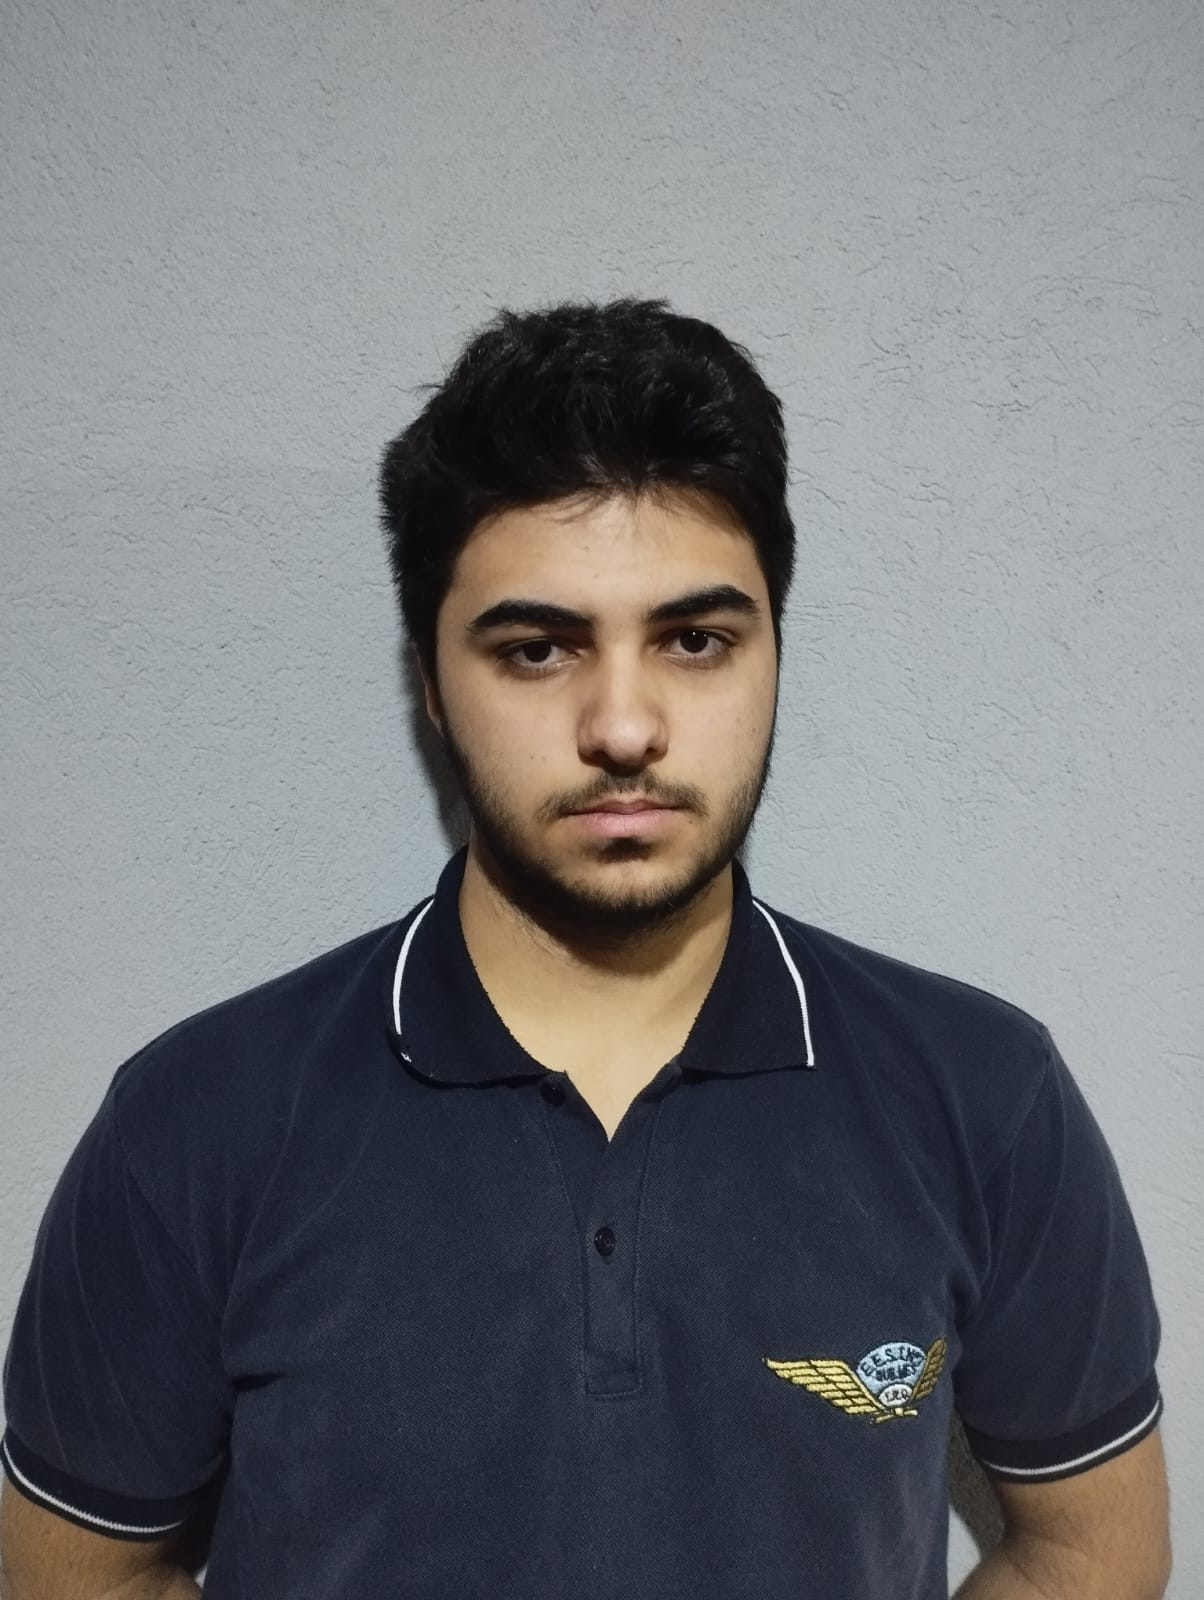
\includegraphics[width=0.25\textwidth]{Preámbulo/Fausto.png} 
                & \SetCell[r=1]{l} Fausto Alvarez Mollo
                &  \\ 
                &  \\
                & \SetCell[r=1]{l}DNI: 46635570
                & \\ 
                &  \\
                & \SetCell[r=1]{l}Mail: faustoalvarezmollo@gmail.com
                &  \\
                &  \\
                & \SetCell[r=1]{l}
\includegraphics[width=0.5cm]{Preámbulo/Linkedin.png}\href{https://www.linkedin.com/in/fausto-alvarez-mollo/}{Linkedin}
                &  \\
                &  \\
                    & \SetCell[r=1]{l}Desarrollo de electrónica y documentación.
                &  \\ 
                &  \\
            \end{tblr}
        \end{table}
        \begin{table}[!ht]
            \begin{tblr}{c c}
                \SetCell[r=10]{} 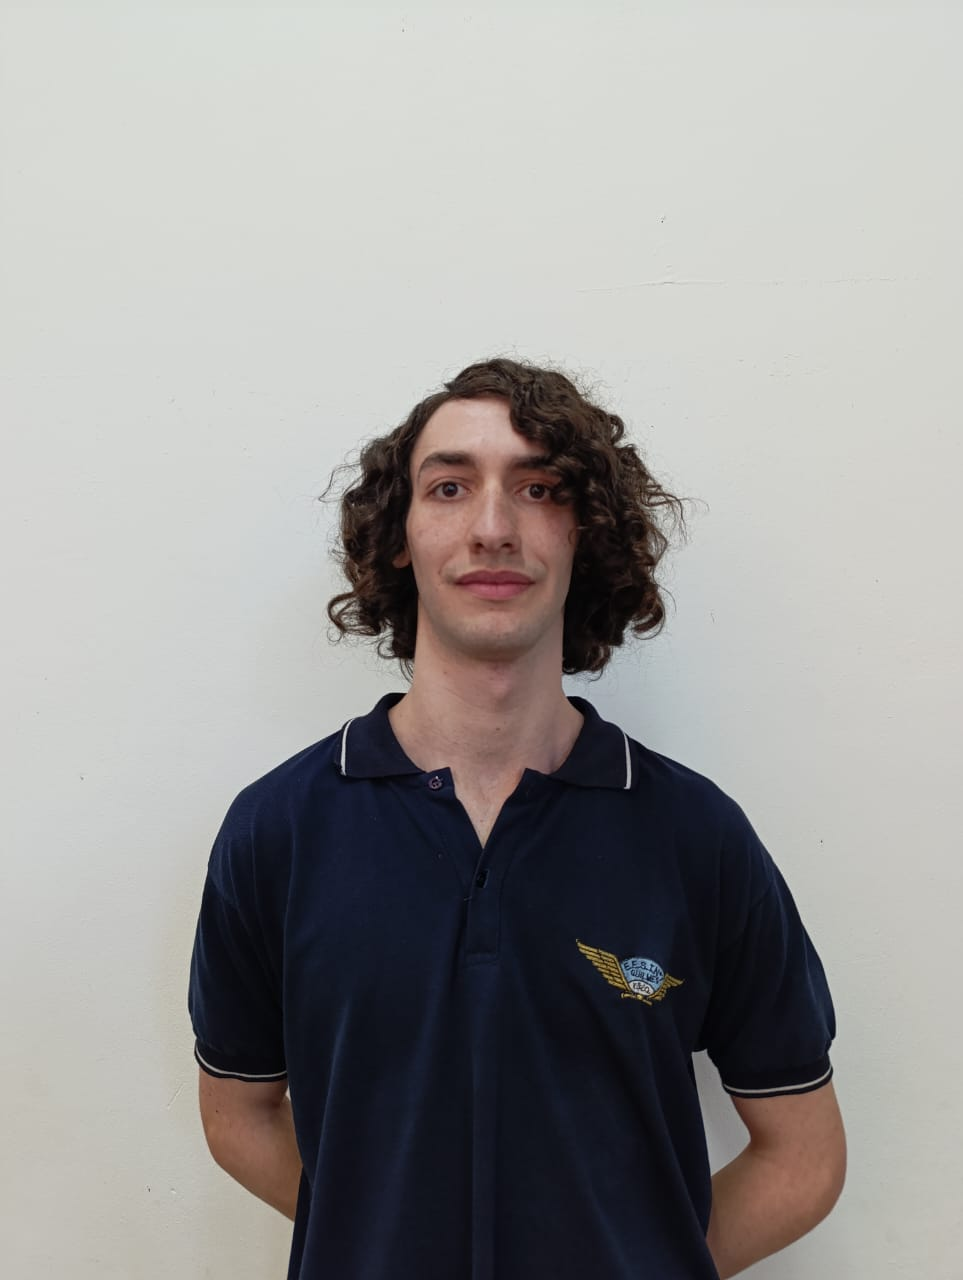
\includegraphics[width=0.25\textwidth]{Preámbulo/Mariano.png} 
                & \SetCell[r=1]{l} Mariano Joaquín Bianqui Kronemberger
                &  \\ 
                &  \\
                & \SetCell[r=1]{l}DNI: 47337141
                & \\ 
                &  \\
                & \SetCell[r=1]{l}Mail: marianobianqui@gmail.com  
                &  \\
                &  \\
                & \SetCell[r=1]{l}
\includegraphics[width=0.5cm]{Preámbulo/Linkedin.png}\href{https://www.linkedin.com/in/mariano-bianqui-5035bb303//}{Linkedin}  
                &  \\
                &  \\
                    & \SetCell[r=1]{l}Desarrollo de Página Web.
                &  \\ 
                &  \\
            \end{tblr}
        \end{table}
        \begin{table}[!ht]
                \begin{tblr}{c c}
                    \SetCell[r=10]{} 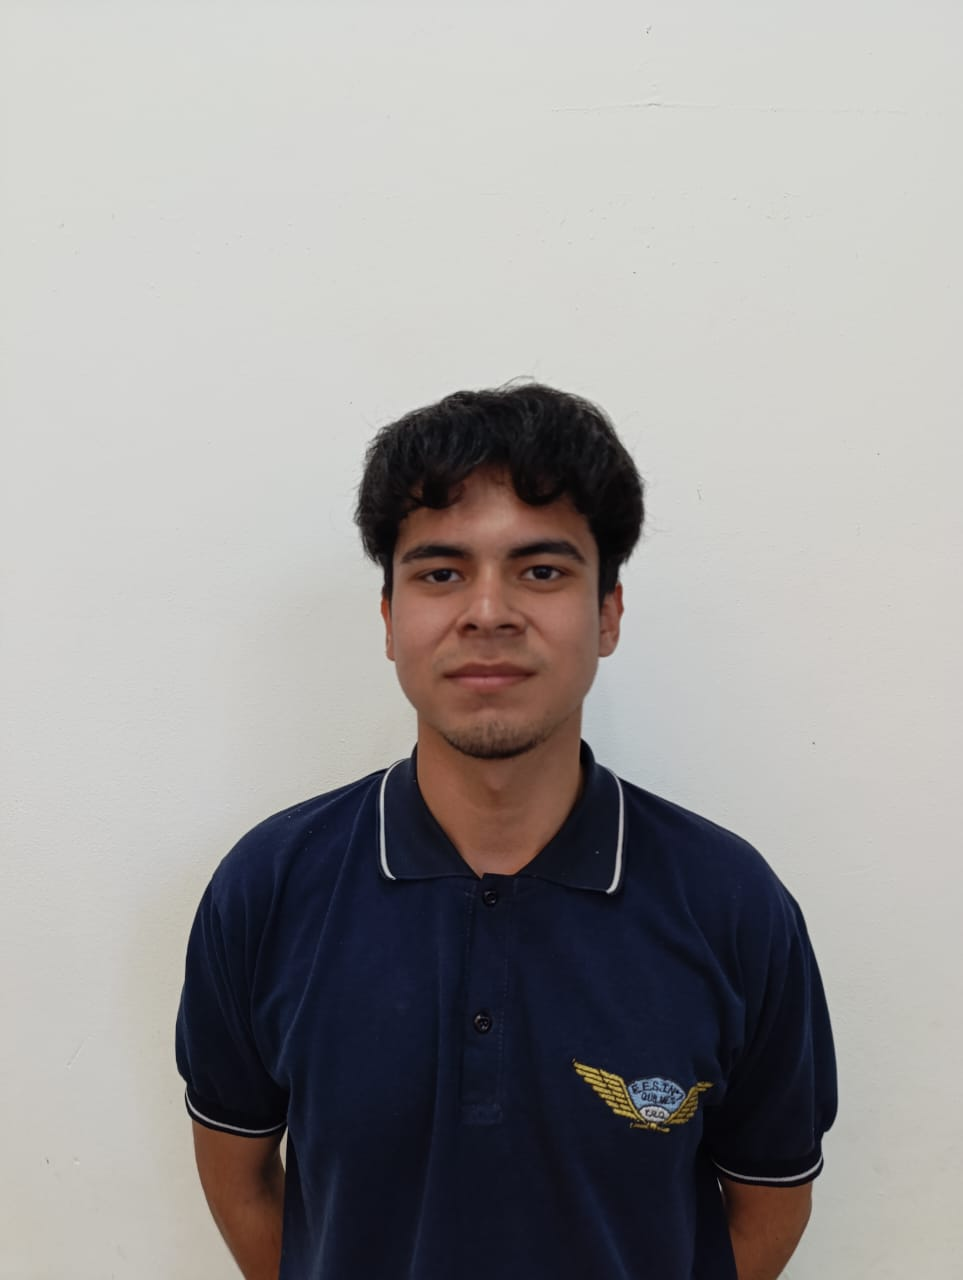
\includegraphics[width=0.25\textwidth]{Preámbulo/Tomás.png} 
                    & \SetCell[r=1]{l} Tomás Joaquín Calleja
                    &  \\ 
                    &  \\
                    & \SetCell[r=1]{l}DNI: 47031210
                    & \\ 
                    &  \\
                    & \SetCell[r=1]{l}Mail: tomascalleja918@gmail.com  
                    &  \\
                    &  \\
                    & \SetCell[r=1]{l}
\includegraphics[width=0.5cm]{Preámbulo/Linkedin.png}\href{https://www.linkedin.com/in/tomás-calleja-5a9894302/}{Linkedin}  
                    &  \\
                    &  \\
                    & \SetCell[r=1]{l}Desarrollo de Aplicación Móvil.
                    &  \\ 
                    &  \\
                \end{tblr}
            \end{table}
            \newpage
            \begin{table}[!ht]
                \begin{tblr}{c c}
                    \SetCell[r=10]{} 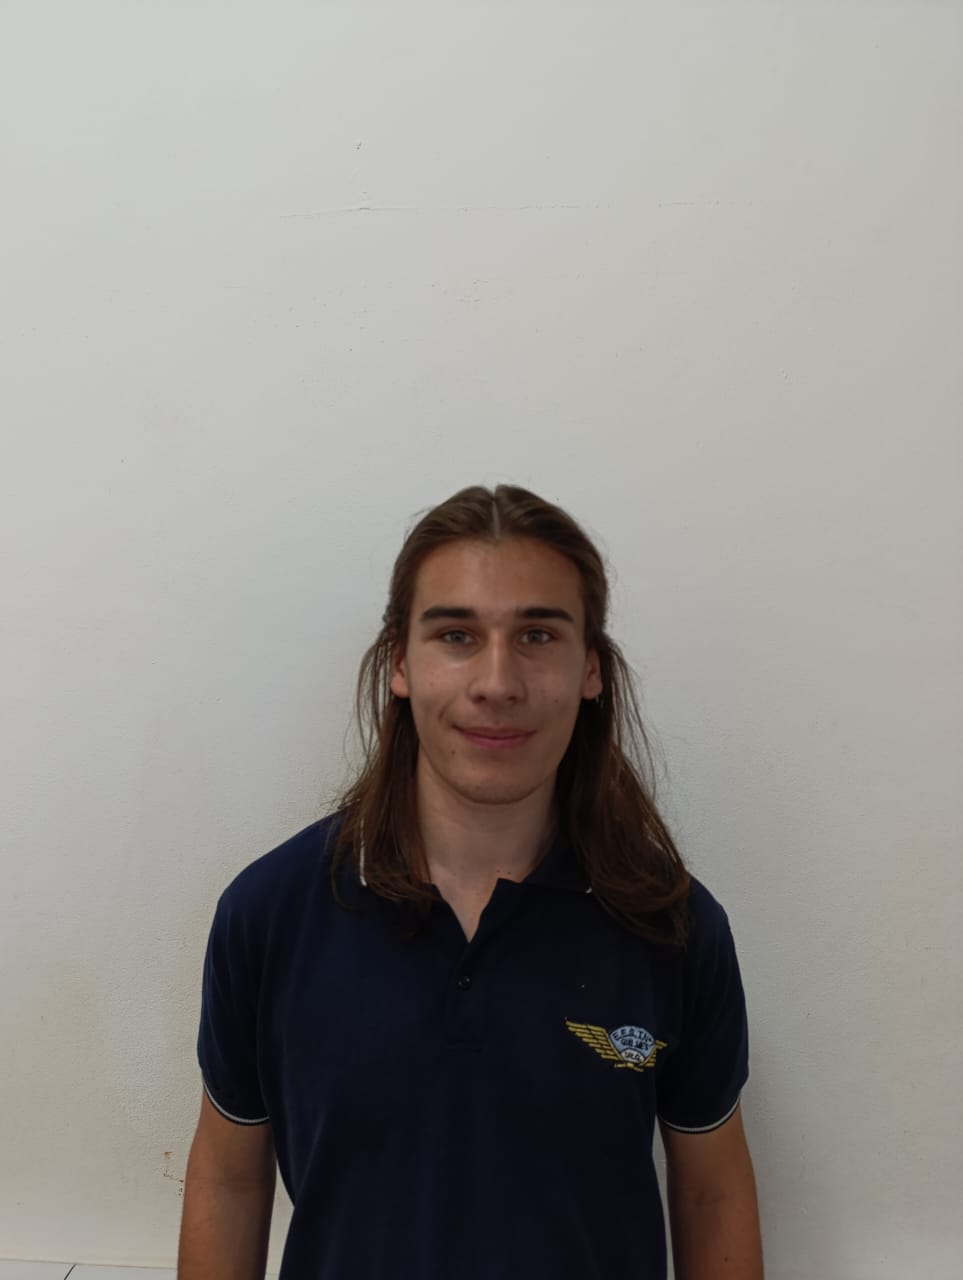
\includegraphics[width=0.25\textwidth]{Preámbulo/Augusto.png} 
                    & \SetCell[r=1]{l} Augusto Donatti
                    &  \\ 
                    &  \\
                    & \SetCell[r=1]{l}DNI: 47057413
                    & \\ 
                    &  \\
                    & \SetCell[r=1]{l}Mail: adonatti2005@gmail.com  
                    &  \\
                    &  \\
                    & \SetCell[r=1]{l}
\includegraphics[width=0.5cm]{Preámbulo/Linkedin.png}\href{https://www.linkedin.com/in/augusto-donatti-54a5bb303/}{Linkedin}
                    &  \\
                    &  \\
                        & \SetCell[r=1]{l}Desarrollo de la Estructura.
                    &  \\ 
                    &  \\
                \end{tblr}
            \end{table}
            \begin{table}[!ht]
                \begin{tblr}{c c}
                    \SetCell[r=10]{} 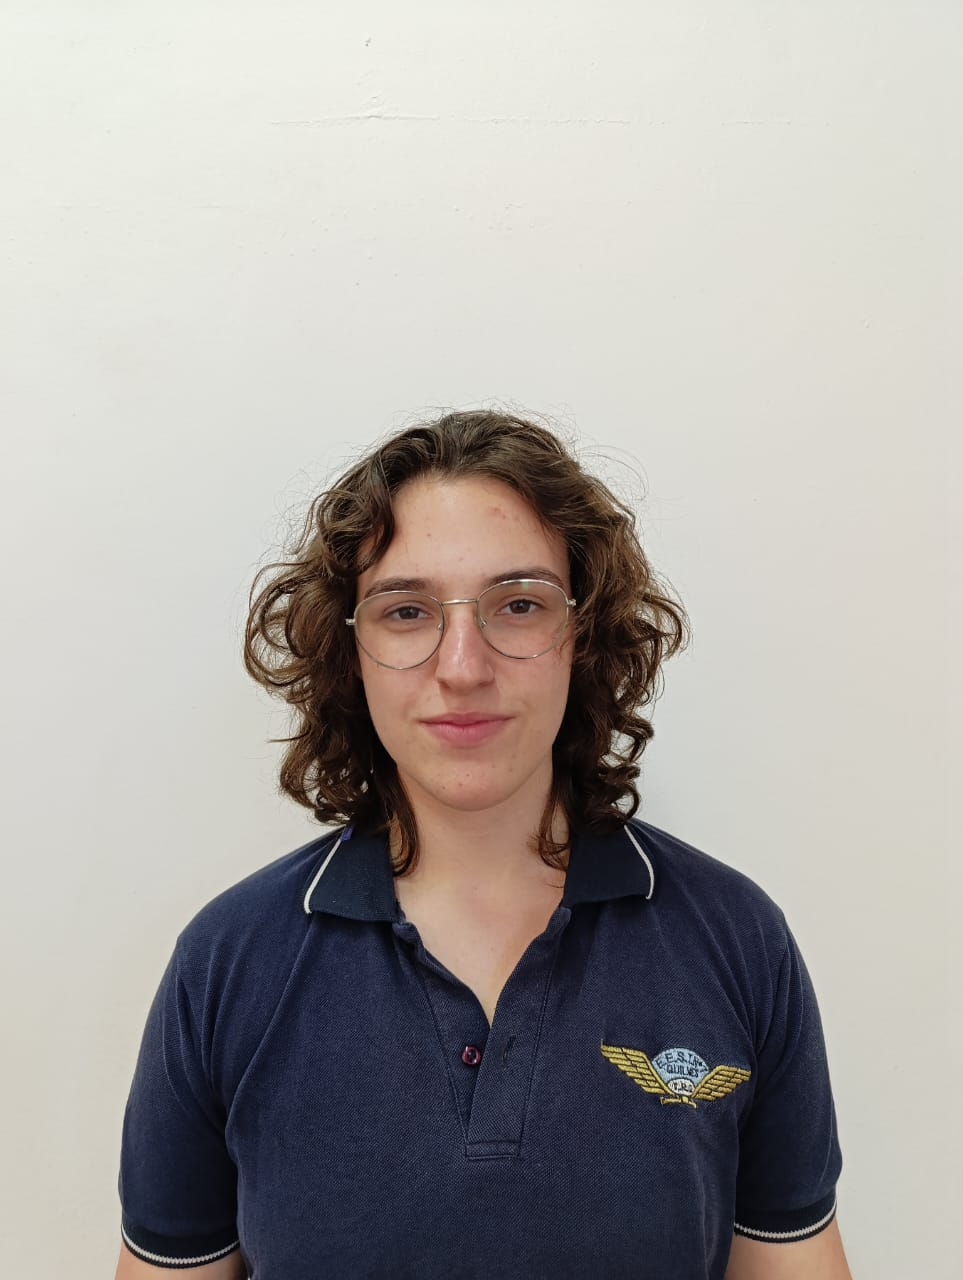
\includegraphics[width=0.25\textwidth]{Preámbulo/Tatiana.png} 
                    & \SetCell[r=1]{l} Tatiana Milena Felizia
                    &  \\ 
                    &  \\
                    & \SetCell[r=1]{l}DNI: 47144482
                    & \\ 
                    &  \\
                    & \SetCell[r=1]{l}Mail: tatianafelizia@gmail.com  
                    &  \\
                    &  \\
                    & \SetCell[r=1]{l}
\includegraphics[width=0.5cm]{Preámbulo/Linkedin.png}\href{https://www.linkedin.com/in/tatiana-felizia-9b29141bb/}{Linkedin}  
                    &  \\
                    &  \\
                        & \SetCell[r=1]{l}Desarrollo de Software e Interfaz.
                    &  \\ 
                    &  \\
                \end{tblr}
            \end{table}
            \begin{table}[!ht]
                \begin{tblr}{c c}
                    \SetCell[r=10]{} 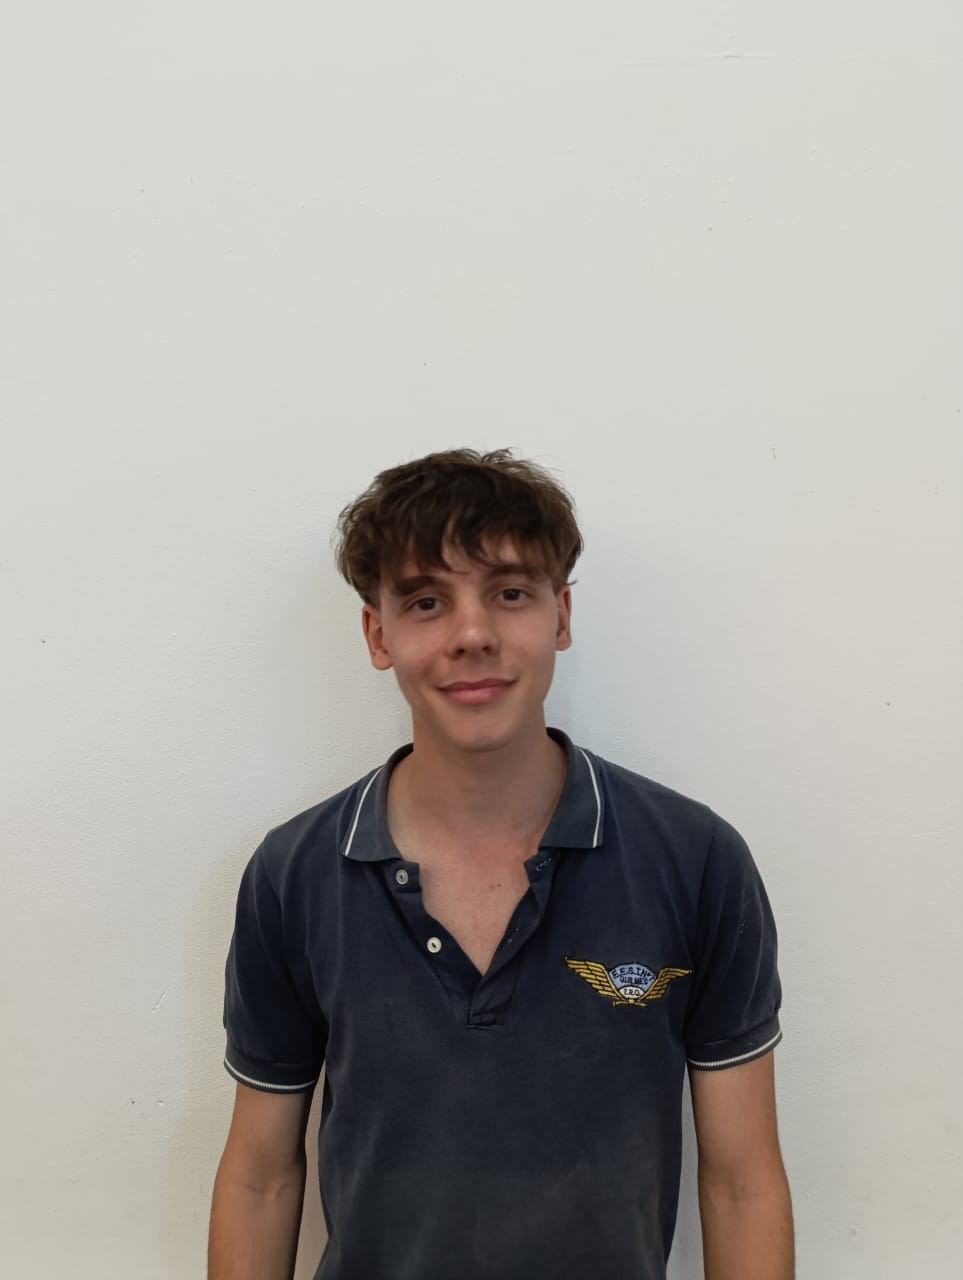
\includegraphics[width=0.25\textwidth]{Preámbulo/Gabriel.png} 
                    & \SetCell[r=1]{l} Gabriel Jerónimo Takashi Sofía
                    &  \\ 
                    &  \\
                    & \SetCell[r=1]{l}DNI: 46904826
                    & \\ 
                    &  \\
                    & \SetCell[r=1]{l}Mail: gabrielsofia19@gmail.com  
                    &  \\
                    &  \\
                    & \SetCell[r=1]{l}
\includegraphics[width=0.5cm]{Preámbulo/Linkedin.png}\href{https://www.linkedin.com/in/gabriel-sofia-035335299/}{Linkedin}  
                    &  \\
                    &  \\
                        & \SetCell[r=1]{l} Desarrollo de Marketing.
                    &  \\ 
                    &  \\
                \end{tblr}
            \end{table}
            
            \begin{figure} [H]
                \centering
                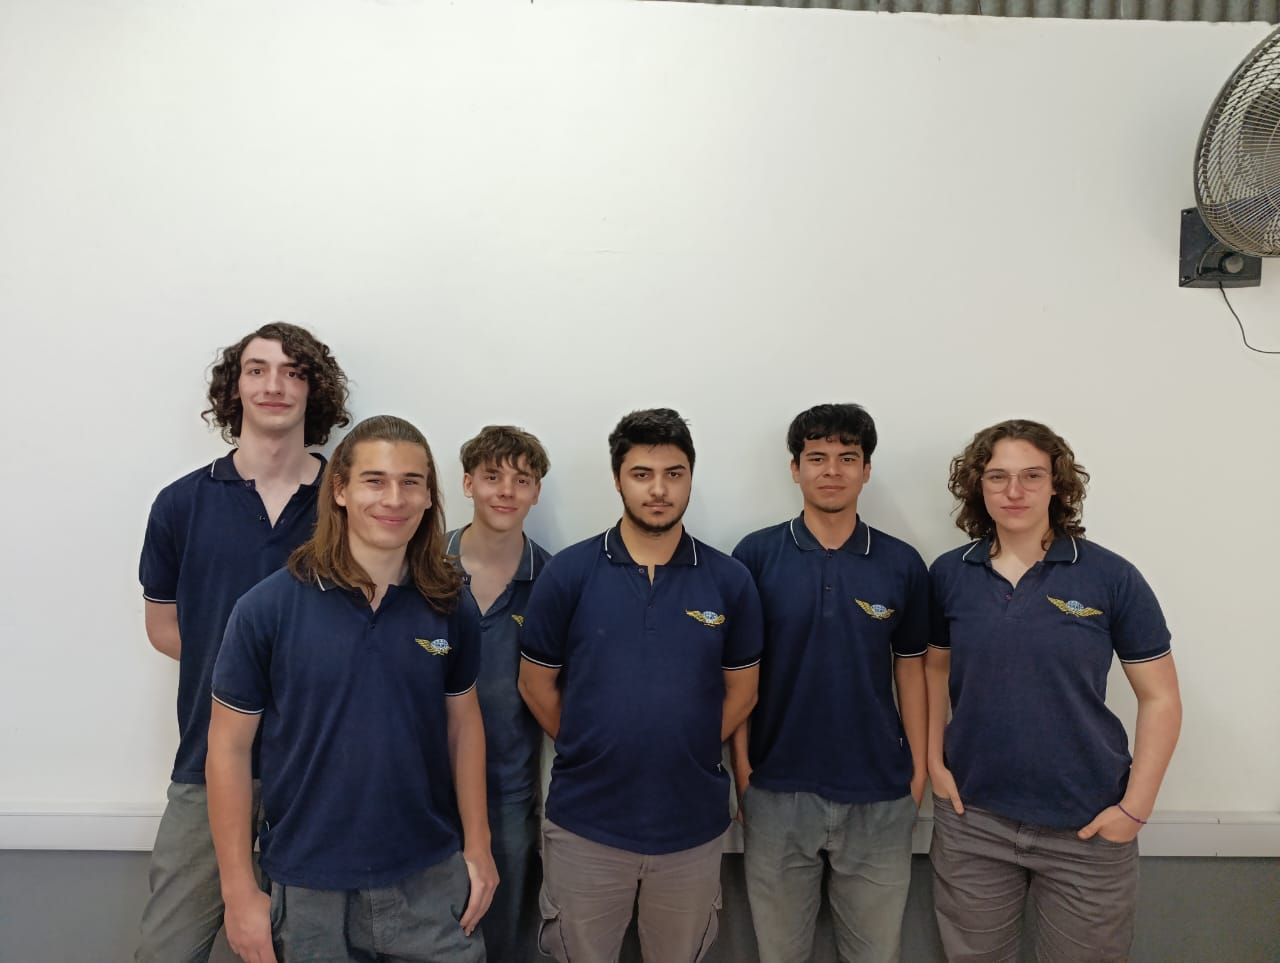
\includegraphics[width=\linewidth]{Preámbulo/Grupal.png}
                \caption{Grupo de \textcolor{dark_violet}{\textbf{GraviCap}}}
            \end{figure}
            \clearpage
        \section{Contacto}
            Mail de Contacto: \textcolor{light_violet}{\textbf{gravicap.arg@gmail.com}}\par
            Cuenta de Instagram: \href{https://www.instagram.com/gravi.cap/}{ \textbf{@gravi.cap}}\par
            Página Web: \href{https://gravicap.vercel.app/home}{\textbf{https://gravicap.vercel.app/home}}\par
            Repositorio de GitHub: \href{https://github.com/impatrq/gravicap}{ \textbf{https://github.com/impatrq/gravicap}}\par
            
        \section{Docentes a cargo}
            \begin{itemize} [label=•]
                \setlength{\itemindent}{1.5em}
                    \item Diego Palmieri
                    \item Carlos Bianco
                    \item Sergio Medina
                    \item Fabrizio Carlassara
                    \item Gabriel Argüello
            \end{itemize}
                
        \section{Agradecimientos}
            Agradecemos a la Asociación Cooperadora del \href{https://www.impatrq.com}{IMPA}.\par
            Agradecemos a \href{https://www.invap.com.ar}{INVAP} y al Ingeniero Marcelo Leo.\par
            Agradecemos a Impulsar por el panel solar.\par
            Agradecemos a todas los programas de difusión que nos brindaron el espacio para que podamos promover el proyecto.\par
            Agradecemos al personal docente y no docente de la institución por el apoyo inmenso que nos dieron.\par

        \section{Información Adicional}
            \subsection{Tiempo total de realización}
                \begin{itemize} [label=•]
                    \setlength{\itemindent}{2.5em}
                        \item \textbf{Día de Inicio}: 18/03/2024
                        \item \textbf{Total de Semanas para la finalización}: 30,28 semanas.
                        \item \textbf{Tiempo individual por semana}: 8 horas.
                        \item \textbf{Tiempo de realización en horas}: 243 horas.
                \end{itemize}
                
            \subsection{Lenguajes de programación utilizados}
                \begin{itemize} [label=•]
                    \setlength{\itemindent}{2.5em}
                        \item \LaTeX
                        \item C++
                        \item C
                        \item HTLM
                        \item CSS
                        \item Vue.js
                        \item React
                        \item Java
                        \item JavaScript
                \end{itemize}
                
                \subsection{Programas utilizados}
                    \begin{itemize} [label=•]
                        \setlength{\itemindent}{2.5em}
                            \item Overleaf
                            \item Visual Studio Code
                            \item Canva
                            \item MarvelApp
                            \item Photoshop
                            \item KiCad
                            \item Inkscape
                            \item Ionic
                            \item Putty
                            \item PlatformIO
                    \end{itemize}
\chapter{Introducción}
    
        \section{\textcolor{dark_violet}{\textbf{GraviCap}}, ¿Qué es?}
            \textcolor{dark_violet}{\textbf{GraviCap}} consiste en un condensador de energía gravitatoria junto a un sistema de control de consumo.\par
            Un condensador de energía gravitatoria, o batería de gravedad es una estructura que eleva una carga consumiendo energía eléctrica, para luego almacenarla en forma de energía potencial gravitatoria. El sistema de control de consumo, revisa constantemente el consumo de energía de la red, eligiendo el momento indicado para soltar la carga, que generará la energía cinética que, luego, será transformada en energía eléctrica por un generador.\par
            \textcolor{dark_violet}{\textbf{GraviCap}}, es un prototipo que ha llevado mucho esfuerzo. Desde sus inicios con una ardua investigación hasta su construcción. Este esfuerzo no se limita solo a la construcción de un prototipo, sino que \textcolor{dark_violet}{\textbf{GraviCap}} busca generar un impacto significativo en la forma en que almacenamos energía a nivel mundial. Tal como se detalla en Alcances (\ref{Alc}), \textcolor{dark_violet}{\textbf{GraviCap}} no solo tiene el \textbf{potencial de transformar el almacenamiento de energía} en Argentina, aprovechando las condiciones geográficas favorables del país, sino también de posicionar a nuestro proyecto como una referencia en el ámbito internacional. Al adoptar un enfoque innovador y sostenible, creemos que \textcolor{dark_violet}{\textbf{GraviCap}} puede desempeñar un papel clave en la transición hacia un futuro energético más limpio y eficiente.\par

        \section{Alcances}
        \label{Alc}
            \subsection{Impacto en Argentina}
                La Argentina posee condciones geográficas muy favorables para la implementación de \textbf{energías renovables}, como la solar y la eólica, en las que \textcolor{dark_violet}{\textbf{GraviCap}} podría ser utilizado para expandir las capacidades del suministro energético argentino.\par
                Por ejemplo, \textcolor{dark_violet}{\textbf{GraviCap}} podría aprovechar zonas como:\par
                \begin{itemize} [label=•]
                    \setlength{\itemindent}{1.5em}
                    
                    \item \textbf{Cordillera de los Andes}: La región montañosa de los Andes es ideal para la instalación de baterías gravitatorias debido a su topografía pronunciada y grandes diferencias de altitud. El uso de sistemas como \textcolor{dark_violet}{\textbf{GraviCap}} en esta zona permitiría almacenar energía de manera eficiente, utilizando el desnivel natural de las montañas.\par
                    \item \textbf{Región Patagónica}: La Patagonia, conocida por sus fuertes vientos, es un punto clave para la generación de energía eólica. La instalación de \textcolor{dark_violet}{\textbf{GraviCap}} en esta región permitiría almacenar la energía producida durante los picos de viento, asegurando un suministro constante, incluso en momentos de baja producción.\par
                    \item \textbf{Noroeste Argentino}: Esta región combina un alto potencial solar y una topografía favorable con cerros y mesetas, lo que la convierte en un lugar ideal para la combinación de energía solar y almacenamiento gravitatorio. En zonas como Jujuy y Salta, la alta irradiación solar podría generar electricidad durante el día, que luego sería almacenada por \textcolor{dark_violet}{\textbf{GraviCap}} para su uso durante la noche o en días nublados.\par
                    \item \textbf{Cuyo}: Las provincias de San Juan y Mendoza, además de tener un alto potencial para la energía solar, también cuentan con relieves montañosos que permiten una fácil implementación de \textcolor{dark_violet}{\textbf{GraviCap}}. La combinación de ambos factores ofrecería una solución integrada para el almacenamiento y el aprovechamiento de energía renovable, mejorando la autosuficiencia energética de la región.\par
                \end{itemize}

            \subsection{Impacto Mundial}
                \textcolor{dark_violet}{\textbf{GraviCap}} se presenta como un innovador prototipo de batería gravitatoria, con el objetivo de posicionar a la Argentina en la vanguardia del almacenamiento de energía y las \textbf{energías renovables}. Este proyecto no solo explora una tecnología emergente, sino que también introduce una nueva corriente de pensamiento en el ámbito global, proponiendo soluciones sostenibles y eficientes frente a los desafíos energéticos contemporáneos. \textcolor{dark_violet}{\textbf{GraviCap}} busca ampliar los horizontes del almacenamiento de energía, aprovechando la fuerza de la gravedad como una fuente renovable, y apunta a generar un impacto significativo en la transición hacia sistemas energéticos más limpios y ecológicos. A través de este enfoque, se abre la posibilidad de fortalecer el rol de Argentina en la adopción de tecnologías de vanguardia, impulsando la innovación en el sector energético tanto a nivel local como internacional.\par
            \subsection{Impacto Social}
                La implementación de la tecnología de \textcolor{dark_violet}{\textbf{GraviCap}} en Argentina podría tener un profundo impacto social, al abordar varios desafíos clave relacionados con el desarrollo sostenible, la equidad energética y la creación de oportunidades económicas.\par
                \begin{enumerate}
                    \setlength{\itemindent}{2.5em}
                    
                    \item \textbf{Acceso a energía limpia y asequible}: \textcolor{dark_violet}{\textbf{GraviCap}} ofrecería una solución innovadora para el almacenamiento de energía renovable, facilitando el acceso a fuentes de energía más limpias y sostenibles. Esto contribuiría a reducir la dependencia de combustibles fósiles, lo que impactaría directamente en la disminución de la huella de carbono y en la mejora de la calidad del aire, con efectos positivos en la salud pública y el bienestar de las comunidades, especialmente en áreas rurales o con dificultades para acceder a fuentes de energía convencionales.\par
                    \item \textbf{Desarrollo económico y generación de empleo}: La fabricación, implementación y mantenimiento de esta tecnología fomentaría la creación de empleo en diversas áreas, desde la ingeniería hasta la instalación y el mantenimiento de los sistemas, generando nuevas oportunidades laborales en sectores emergentes. Además, al posicionar a Argentina como pionera en tecnologías de almacenamiento de energía gravitatoria, se abriría el camino para atraer inversiones y fomentar el desarrollo de una industria energética renovable más robusta y diversificada.\par
                    \item \textbf{Descentralización energética}: Al permitir el almacenamiento eficiente de \textbf{energías renovables}, como la eólica o la solar, \textcolor{dark_violet}{\textbf{GraviCap}} podría impulsar la creación de sistemas de energía descentralizados. Esto favorecería la autonomía energética de comunidades aisladas o con escasa infraestructura eléctrica, mejorando la calidad de vida y proporcionando a las regiones más alejadas una herramienta crucial para su desarrollo.\par
                    \item \textbf{Educación e innovación tecnológica}: La introducción de esta tecnología también incentivaría la formación de nuevas generaciones de técnicos e ingenieros especializados en \textbf{energías renovables}. Esto no solo elevaría el nivel educativo del país, sino que también fomentaría una cultura de innovación y sostenibilidad, inspirando a investigadores y emprendedores locales a explorar nuevas soluciones tecnológicas para los retos energéticos y medioambientales.\par
                    \item \textbf{Reducción de la pobreza energética}: Al facilitar un acceso más estable y accesible a fuentes de energía renovable, \textcolor{dark_violet}{\textbf{GraviCap}} podría contribuir a reducir la pobreza energética en Argentina. Esto es especialmente relevante en comunidades vulnerables, que podrían beneficiarse de un suministro energético más confiable y a costos más bajos, mejorando su calidad de vida.
                \end{enumerate}
                En resumen, \textcolor{dark_violet}{\textbf{GraviCap}} tiene el potencial de ser una herramienta transformadora no solo en términos tecnológicos, sino también en su capacidad para mejorar el bienestar social, fomentar el crecimiento económico y consolidar el papel de Argentina en la lucha global contra el cambio climático.\par
        
        \section{Beneficios}
            \textcolor{dark_violet}{\textbf{GraviCap}} es un proyecto ideado para acompañar a los distintos generadores de energías renovables, adaptándose a las dimensiones que desee utilizar su consumidor acorde a la capacidad de su red eléctrica. Procura resguardar su huella de carbono al estar conformado por piezas simples sin requerimientos técnicos en demasía. Gracias a esto, pueden estar fabricadas por materiales reutilizados, derivados de materias primas locales o biomateriales. Permite prescindir aquellos materiales que perjudican al ambiente durante su producción o con su posterior desecho, ya que no hay materiales peligrosos para proteger.\par
            Almacenar energía gravitatoria nos permite ser también sustentables, ya que depende únicamente de un peso y la altura. El almacenamiento de energía es una problemática cada vez mayor, y con un planeta con crecientes problemas ambientales surgen problemas si estos son contaminantes.\par
            
            
        \section{¿Por qué \textcolor{dark_violet}{\textbf{GraviCap}}?}
            Siempre que se presenta un producto innovador surge una problematica, ¿Por qué usarlo y no usar un método más convencional?\par
            En este caso, ¿Por qué usar \textcolor{dark_violet}{\textbf{GraviCap}} y no una batería convencional?\par
            
            \subsection{Almacenamiento de Energías Renovables}
                Con la cada vez más creciente demanda y utilización de las energías renovables, como la eólica y la solar, nos encontramos con el principal problema que conllevan. Al depender de fenómenos meteorológicos para producir energía, se vuelven impredecibles y variables, cuando la red eléctrica exige una entrega constante.\par
                Para rectificar su entrega, la solución predilecta es acompañar al generador de una batería que almacene el excedente producido en momentos de superávit energético, y entregue en los momentos de déficit.\par
                Así surge una situación compleja: ¿Cómo almacenamos energía? Se presentan dos principales escenarios:\par

                \begin{itemize} [label=•]
                    \setlength{\itemindent}{1.5em}
                        \item Almacenar de forma eficiente el exceso: Cuando las condiciones son tan favorables que se produce más de lo que se demanda.\par
                        \item Recuperar el exceso: Cuando las condiciones no son favorables, la energía producida no es suficiente para cubrir la demanda.\par
                \end{itemize}
                
            \subsection{¿Por qué es necesario?}
                 El almacenamiento de energía representa una excelente oportunidad para la integración de fuentes renovables en el sistema eléctrico. No solo implica una mejora en la flexibilidad y seguridad del sistema, sino también un aumento en su eficiencia global.\par
                 Desde la perspectiva de las empresas de servicios públicos, la estrategia de almacenamiento ofrece una manera efectiva de reducir los costos de generación eléctrica. Almacenar la electricidad durante las horas valle, es decir, durante la noche cuando la demanda es baja, y luego descargarla durante las horas punta del día, cuando la demanda alcanza su pico máximo, se traduce en beneficios sustanciales. Cuanto mayor sea la disparidad entre la demanda en las horas punta y valle, mayores serán los beneficios derivados del almacenamiento de energía.\par
                 Además de los beneficios económicos, esta práctica también conduce a una generación más uniforme de energía, lo que a su vez mejora la eficiencia general del sistema. La capacidad de suavizar las fluctuaciones en la generación de energía contribuye a una operación más estable y confiable del sistema eléctrico en su conjunto. En resumen, el almacenamiento de energía no solo ofrece ventajas económicas, sino que también promueve una operación más eficiente y sostenible del sistema eléctrico.\par
                 
            \subsection{Beneficios del almacenamiento}
                 Para el transporte y la distribución energética:\par
                    
                \begin{itemize} [label=•]
                    \setlength{\itemindent}{1.5em}
                        \item Aumentar la eficiencia de la red, cuando hay congestión en la red no hay tiempo para satisfacer la demanda y el almacenamiento ayuda a liberar esta congestión.\par
                        \item Aumentar la capacidad efectiva de transporte y distribución debido a las posibilidades de carga y descarga a alta velocidad.\par
                        \item Incrementar la capacidad de distribuir energía cerca del consumo, reduciendo las pérdidas técnicas y la congestión.\par
                \end{itemize}
                    
                 Para el consumidor:\par
                    
                \begin{itemize} [label=•]
                    \setlength{\itemindent}{1.5em}
                        \item Continuidad de suministro, si se producen fallos en las redes el almacenamiento ayudará a mantener constante el suministro.\par
                        \item Reducción de costes, las empresas eléctricas pueden fijar precios variables en el tiempo (menor precio por la noche y mayor por el día) para dar un incentivo a los consumidores; al aplanar la curva de la demanda.\par
                \end{itemize}
                    
                 Para la generación de energía:\par
                 
                 \begin{itemize} [label=•]
                    \setlength{\itemindent}{1.5em}
                        \item Incrementar la fiabilidad del sistema, cuando la generación es mediante una fuente de energía renovable, sol o viento, con el almacenamiento se asegura el suministro, aunque no brille el sol o no haya viento.\par
                        \item Arbitraje de energía en tiempo real.\par
                        \item Regulación de tensión y corriente.\par
                \end{itemize}

            \subsection{Contaminación de Baterías}
                En el panorama actual, el uso de baterías ha experimentado un crecimiento exponencial, impulsado por avances tecnológicos, la creciente demanda de dispositivos electrónicos portátiles y la transición hacia vehículos eléctricos. Este aumento en la adopción de baterías como fuente de energía móvil ha generado una preocupación creciente sobre la gestión adecuada de los residuos resultantes de su desecho.\par
                Las baterías, en su variedad de formas y tipos, contienen una combinación de elementos que pueden ser perjudiciales para el medio ambiente y la salud humana. Entre estos componentes se encuentran el mercurio (Hg), el cadmio (Cd), el plomo (Pb), el níquel (Ni), el manganeso (Mn) y el zinc (Zn), sustancias que, si no se manejan adecuadamente, pueden contaminar el suelo y el agua, y representar un riesgo para la vida silvestre y los ecosistemas.\par
                Según el tipo de electrolito que contienen, las baterías pueden ser clasificadas en secas o húmedas. Las baterías de uso doméstico típicamente tienen electrolito seco, el cual puede ser alcalino o ácido, como se detalla en la tabla \ref{tab:1}. En algunos casos particulares, el electrolito ácido puede estar contenido en un gel, el cual está cubierto por un material permeable o de fibra de vidrio para su seguridad y manejo adecuado.\par
                La duración y el tipo de manejo requerido también son factores determinantes en la clasificación de las baterías, agrupándolas en primarias o desechables, y secundarias o recargables. Por lo general, para propósitos comerciales y técnicos, las baterías son tipificadas según sus componentes, lo cual puede observarse en las tablas \ref{tab:1} y \ref{tab:2}.\par
                
                \begin{table}[!htbp]
                    \centering
                    \begin{tabular}{|c|c|}
                         \hline
                         Tipos de Pila &  Componentes Principales\\
                         \hline
                         & Zinc 17\% (Anódo) \\
                         & Dióxido de Manganeso 29\% (Cátodo) \\
                         & Carbón 7\%\\
                         Carbono-Zinc & Mercurio 0,01\% (Anódo, Cátodo y Electrolito) \\
                         (C-Zn) & Cadmio 0,08\%\\
                         & Cloruro de Amonio (Electrolito)\\
                         & Plástico y Lámina 26\%\\
                         \hline
                         & Zinc 14\% (Anódo)\\
                         & Dióxido de Manganeso 22\% (Cátodo)\\
                         & Carbón 2\%\\
                         Alcalinas & Mercurio 0,5\% a 1\% (Anódo)\\
                         & Hidróxido de Potasio (Electrolito)\\
                         & Plástico y Lámina 42\%\\
                         \hline
                         & Óxido de Mercurio (33\% Hg) (Cátodo)\\
                         Óxido de Mercurio & Zinc 11\% (Anódo)\\
                         (HgO) & Hidróxido de Potasio o Hidróxido de Sodio (Electrolito)\\
                         & Plástico y Lámina 29\%\\
                         \hline
                         & Zinc 30\% (Anódo)\\
                         & Óxigeno (Del Aire, Cátodo)\\
                         Zinc-Aire & Mercurio 1\%\\
                         (Zn-Aire) & Plata 1\%\\
                         & Plástico y Lámina 67\%\\
                         & Cloruro de Sodio o Hidróxido de Sodio (Electrolito)\\
                         \hline
                         & Zinc 10\% (Anódo)\\
                         & Óxido de Plata 27\% (Cátodo)\\
                         Óxido de Plata & Mercurio 1\%\\
                         (AgO2) & Cloruro de Sodio o Hidróxido de Sodio (Electrolito)\\
                         & Plástico y Lámina 29\%\\
                         \hline
                         & Litio 10\% a 30\%\\
                         Litio (Li) & Dióxido de Manganeso (Cátodo)\\
                         & Plástico y Lámina 29\%\\
                         \hline
                    \end{tabular}
                    \caption{Componentes principales de las pilas primarias (Desechables)}
                    \label{tab:1}
                \end{table}

                \begin{table}[!htbp]
                    \centering
                    \begin{tabular}{|c|c|}
                         \hline
                         & Cadmio (Cd) 18\%\\
                         Níquel-Cadmio (Ni-Cd) & Níquel (Ni) 20\%\\
                         & Hidróxido de Potasio o de Sodio\\
                         \hline
                         Níquel-Metal Hidruro & Níquel (Ni) 25\%\\
                         (Ni-MH) & Hidróxido de Potasio\\
                         \hline
                         & Óxido de Litio-Cobalto (Cátodo)\\
                         Ión-Litio (Ión-Li) & Carbón altamente cristalizado (Anódo)\\
                         & Solvente orgánico (Electrolito)\\
                         \hline
                         Plomo & Plomo\\
                         (Pb) & Ácido Sulfúrico\\
                         \hline
                    \end{tabular}
                    \caption{Componentes principales de las pilas secundarias (Recargables)}
                    \label{tab:2}
                \end{table}
                \newpage
                Las pilas de C-Zn, utilizadas en los dispositivos electrónicos más comunes, son propensas a quemarse por sobrecalentamiento. Una vez quemadas liberan altas cantidades de metales pesados al ambiente en una reacción exotérmica incontrolable. Existen estudios que indican que el 35\% de la contaminación de mercurio producida es a causa de la quema de baterías de C-Zn junto con la basura común.\par
                También, estudios médicos han demostrado que un alto nivel de mercurio en la sangre provoca cambios de personalidad, pérdida de visión, sordera, problemas en los riñones y pulmones. Es altamente peligroso para las mujeres embarazadas. La vía principal de exposición al mercurio elemental es por inhalación de sus vapores. Cerca del 80\% de los vapores inhalados es absorbida por los tejidos pulmonares. Este vapor también penetra con facilidad la barrera de sangre del cerebro y su neurotoxicidad está bien documentada.\par
                La absorción intestinal de mercurio elemental es baja. El mercurio elemental puede oxidarse en los tejidos corporales a la forma divalente inorgánica.\par
                Se han observado trastornos neurológicos y de comportamiento en seres humanos tras inhalación de vapor de mercurio elemental. Algunos de los síntomas son: temblores, labilidad emocional, insomnio, pérdida de la memoria, cambios en el sistema neuromuscular y dolores de cabeza. Se han observado asimismo efectos en el riñón y la tiroides. Las exposiciones altas también han ocasionado mortalidad.\par
                La mayoría de las pilas y baterías recargables, actualmente carecen de mercurio.\par
                Sin embargo contienen hasta un 15\% níquel y cadmio, dos metales pesados tóxicos. El cadmio emitido al ambiente se disuelve parcialmente en el agua pero no se degrada, por lo que las plantas y animales asimilan este metal, permaneciendo en el organismo durante largo tiempo.\par
                El cadmio es calificado como cancerígeno, causante de trastornos en el aparato digestivo, produce lesiones en los pulmones. Al ingerirse se acumula en los riñones. El efecto adverso más común de exposición al níquel es una reacción alérgica, algunas personas podrían sufrir ataques de asma luego de períodos de exposición. Ciertos compuestos del níquel son posiblemente carcinógenos para los seres humanos, La exposición a niveles de manganeso muy altos durante largo tiempo ocasiona perturbaciones mentales y emocionales, y provoca movimientos lentos y faltos de coordinación.\par
                Dado que el mayor volumen consumido de pilas son alcalinas y de carbón-zinc (aproximadamente el 76\% del consumo total), el óxido de manganeso contenido en ellas es el contaminante que en mayor volumen se ha liberado al medio ambiente.\par
                Las pilas tardan más de 1000 años en degradarse, sus componentes son altamente contaminantes y no se degradan, pueden empezar a separarse luego de 50 años al aire libre. Los metales de mayor preocupación, presentes en las pilas de uso doméstico son el Hg, Cd, Mn, Ni, y Zn.\par 
                Aunque el litio en sí mismo no es considerado como un contaminante, es importante tener en cuenta que muchos de los componentes empleados en las baterías que contienen litio pueden ser altamente perjudiciales para el medio ambiente y la salud humana. Por ejemplo, el cobalto, un metal comúnmente utilizado en este tipo de baterías, es altamente tóxico. La exposición al cobalto puede provocar una serie de efectos adversos para la salud, como vómitos, náuseas, problemas de visión, trastornos cardíacos y daños en la tiroides. Esta información destaca la importancia de no solo considerar el impacto ambiental directo de las baterías, sino también los efectos secundarios asociados con los materiales utilizados en su fabricación.\par
                            
        \section{Estado del Arte}
            Actualmente, en el ámbito global, existe únicamente una empresa que se dedica a la construcción de Baterías de Gravedad conocida como \href{https://www.energyvault.com}{Energy Vault} con sede en Suiza. La empresa ha logrado construir baterías en el mundo como \href{https://www.energyvault.com/projects/zhangye}{una batería en China} o \href{https://www.renewableenergyworld.com/storage/energy-vault-lands-partnership-for-building-based-gravity-storage/}{un proyecto en Australia}.\par
            \begin{figure} [ht]
                \centering
                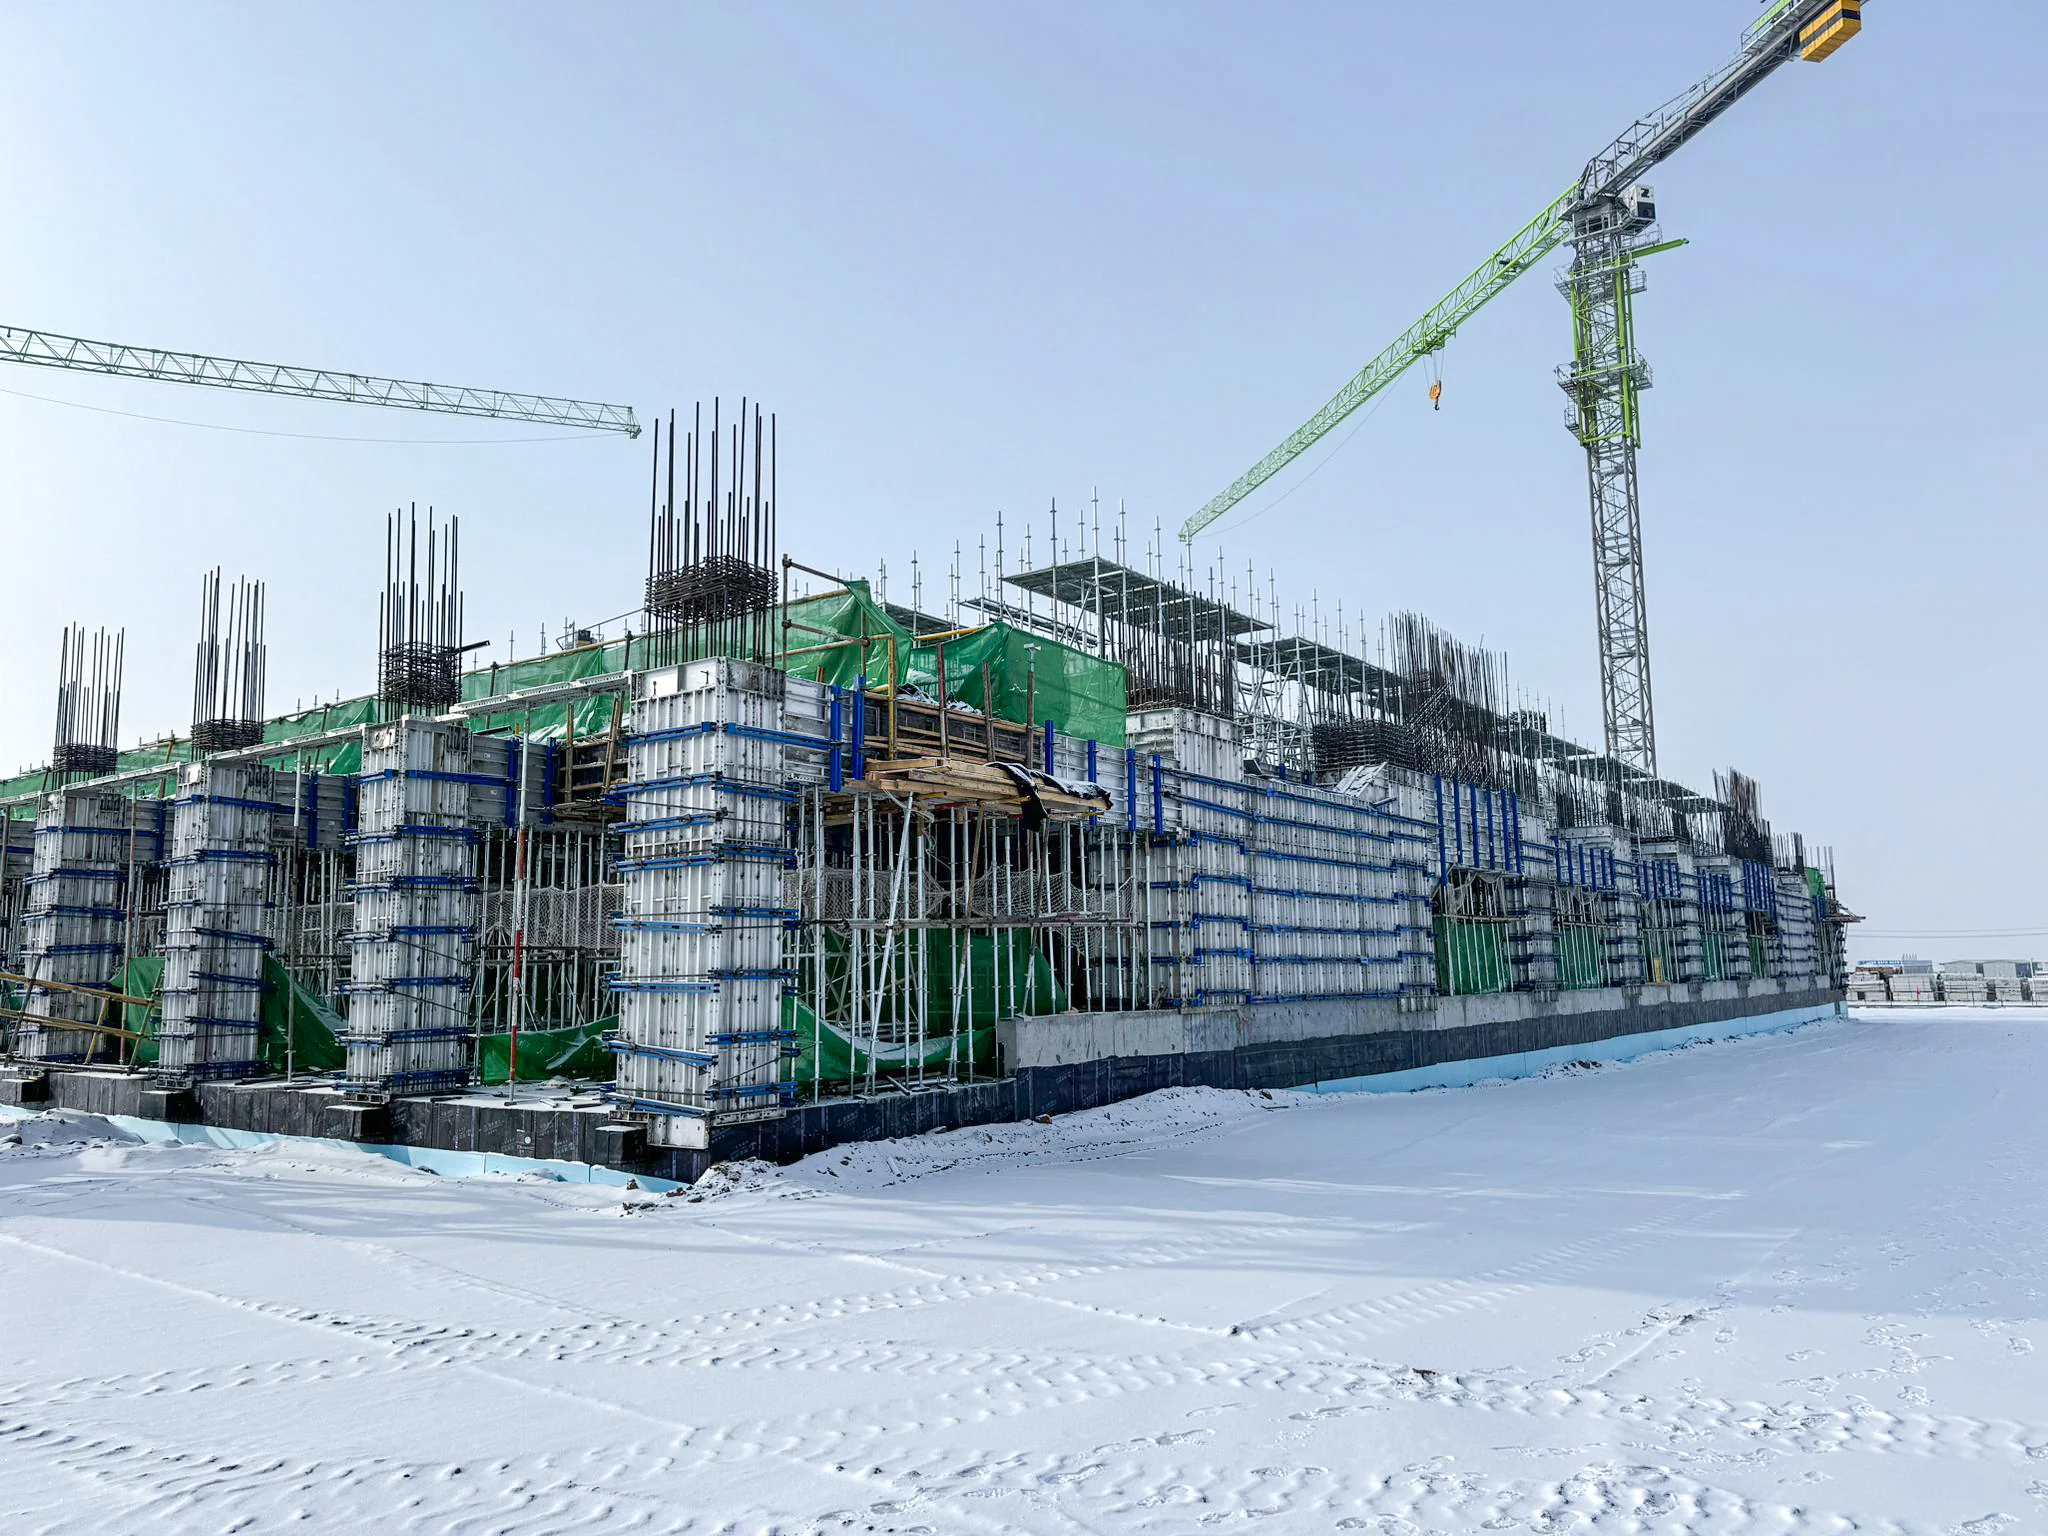
\includegraphics [width=10cm]{Introducción/Zhangye.png}
                \caption{Proyecto de Construcción en Zhangye, China}
                \label{fig:Zhangye}
            \end{figure}
            Energy Vault no se dedica a la comercialización directa de estas, sino que se construyen a pedido del usuario.\par
            En \textcolor{dark_violet}{GraviCap}, nuestro enfoque es totalmente opuesto. Nos esforzamos por empoderar al usuario brindándole el conocimiento necesario para construir su propio sistema y proporcionándole una guía detallada sobre los materiales adecuados para llevar a cabo el proyecto.\par

        \section{Implementación}
            La implementación de este tipo de tecnología en un inicio puede parecer costosa, pero los beneficios a largo plazo son indudables. La introducción de esta propuesta al mercado argentino, como se ha detallado en muchas ocasiones a lo largo de los textos anteriores, no solo tiene el potencial de posicionar a Argentina como un referente en el campo del almacenamiento de energías renovables, sino también de fortalecer su autosuficiencia energética. Al adoptar soluciones como \textcolor{dark_violet}{\textbf{GraviCap}}, se estaría optimizando la capacidad del país para aprovechar sus recursos naturales, como la energía solar y eólica, y al mismo tiempo, reducir la dependencia de fuentes de energía no renovables y contaminantes.\par
        
        \section{Usuarios}
            \textcolor{dark_violet}{\textbf{GraviCap}} presenta tres enfoques principales (que también llamamos \textcolor{light_violet}{\textbf{\textit{3C}}}) al futuro usuario del sistema:\par
            \begin{enumerate}
                \setlength{\itemindent}{2.5em}
                
                \item \textbf{Conocimiento}.
                \item \textbf{Concientización}.
                \item \textbf{Capacitación}.
            \end{enumerate}
            \subsection{Conocimiento}
                Este enfoque se centra en ofrecer al usuario una comprensión sólida sobre el funcionamiento de \textcolor{dark_violet}{\textbf{GraviCap}} y su papel dentro del sistema energético. El conocimiento abarca no solo los aspectos técnicos, como el proceso de conversión de energía gravitatoria a energía eléctrica, sino también los beneficios medioambientales que ofrece el uso de esta tecnología. Los usuarios serán informados sobre el impacto positivo de \textcolor{dark_violet}{\textbf{GraviCap}} en la reducción de emisiones de carbono, su eficiencia energética y su papel dentro de un sistema más amplio de energías renovables. La difusión de este conocimiento es clave para que los usuarios adopten la tecnología con confianza y se sientan parte de la transición hacia una energía más limpia y sostenible.
            \subsection{Concientización}
                \textcolor{dark_violet}{\textbf{GraviCap}} no solo busca ofrecer una solución tecnológica, sino también crear conciencia sobre la importancia de la sostenibilidad y el uso responsable de los recursos energéticos. Este enfoque busca sensibilizar a los usuarios sobre el impacto ambiental del consumo energético tradicional y cómo el uso de tecnologías limpias, como \textcolor{dark_violet}{\textbf{GraviCap}}, puede ayudar a mitigar los efectos del cambio climático. Se pondrá énfasis en la reducción de la dependencia de combustibles fósiles y en la necesidad de transitar hacia un sistema energético más equilibrado y respetuoso con el medio ambiente. La concientización también incluye la adopción de hábitos energéticos más responsables, fomentando una cultura de ahorro y eficiencia en el uso de la energía.\par
            \subsection{Capacitación}
                \textcolor{dark_violet}{\textbf{GraviCap}} ofrece a sus usuarios la oportunidad de capacitarse en el uso y mantenimiento del sistema. Este enfoque busca no solo que los usuarios comprendan cómo funciona la tecnología, sino también que adquieran las habilidades necesarias para operarla de manera autónoma y eficiente. La capacitación incluirá formación en el montaje, manejo y control de la batería gravitatoria. Además, se proporcionarán guías para el mantenimiento preventivo, asegurando la durabilidad y el buen funcionamiento del sistema a largo plazo. La capacitación también incluye un componente educativo que fomenta el conocimiento sobre energías renovables y su integración en la vida cotidiana.\par
\chapter{Estructura}

    \section{Introducción}
    
        Nuestra estructura está diseñada para aprovechar eficientemente la energía potencial gravitatoria mediante un sistema innovador que convierte dicha energía en electricidad utilizable para el consumidor. Este sistema, que se fundamenta en principios físicos sólidos, se basa en la capacidad de almacenar energía cuando se eleva un peso y liberarla controladamente al permitir que dicho peso descienda. Este proceso de elevación y descenso es crucial, ya que permite la conversión de la energía potencial gravitatoria en energía mecánica. A su vez, esta energía mecánica es transformada en energía eléctrica a través de un generador, completando así el ciclo de conversión.\par
        El concepto de energía potencial gravitatoria se basa en la relación entre la masa del objeto, la altura desde la cual se eleva y la fuerza de gravedad que actúa sobre él. Cuando un peso es elevado, se almacena una cantidad significativa de energía, que puede ser aprovechada posteriormente al liberar el peso y dejar que caiga. Este método de almacenamiento y liberación de energía es no solo eficiente, sino también innovador, ya que utiliza la gravedad, una de las fuerzas fundamentales de la naturaleza, como medio para generar electricidad.\par
        El sistema se configura de tal manera que maximiza la conversión de energía y minimiza las pérdidas durante los procesos de elevación y descenso. Al actuar sobre la energía potencial almacenada en el peso, se logra transformar dicha energía en un flujo eléctrico útil que puede ser utilizado para satisfacer las demandas energéticas de los consumidores. Este proceso, que involucra la mecánica del movimiento y la generación eléctrica, es clave para el funcionamiento de la estructura y para alcanzar los objetivos de sostenibilidad y eficiencia energética que perseguimos.\par
        A través de la implementación de este sistema, buscamos demostrar la viabilidad de las baterías gravitatorias como una alternativa renovable y accesible a otras formas de almacenamiento de energía, contribuyendo así a la transición hacia un futuro más sostenible y respetuoso con el medio ambiente.\par
        
    \section{Fundamentos de la Energía Potencial Gravitatoria}
    
        La energía potencial gravitatoria ($E_p$) es la energía que un objeto posee debido a su posición en un campo gravitatorio. En el caso de una batería gravitatoria, el objetivo es aprovechar esta energía elevando una masa a una cierta altura para luego, cuando la masa desciende, convertir esa energía en energía mecánica, y finalmente en energía eléctrica. La fórmula para calcular la energía potencial gravitatoria es:\par
        
        \begin{equation}
            E_p = mgh
        \end{equation}
        
        Donde:\par
        
        \begin{itemize} [label=•]
            \setlength{\itemindent}{1.5em}
            
            \item $E_p$ es la energía potencial en Joules [$J$].
            \item $m$ es la masa del objeto en kilogramos [$kg$].
            \item $g$ es la aceleración de la gravedad ($9,81 \nicefrac{m}{s^2}$).
            \item $h$ es la altura en metros [$m$].
        \end{itemize}
        
        La energía potencial gravitatoria es directamente proporcional a la masa ($m$) y a la altura ($h$). A mayor masa o mayor altura, se almacena más energía. En este sistema, el peso de 27 kg se eleva hasta una altura de 2,2 metros, por lo que la energía potencial almacenada es:\par

        \begin{equation}
            E_p = 27kg \times 9,81 \nicefrac{m}{s^2} \times 2,2m = 582,69 J
        \end{equation}
        
        Esto significa que, cuando el peso está en su posición más alta, el sistema puede almacenar 582.69 Joules de energía, la cual se puede liberar cuando el peso desciende. Si se aumenta la altura o la masa, la energía potencial se incrementará de manera proporcional.\par
        Para un sistema más complejo, donde se utilizan varias masas a distintas alturas, la energía potencial total del sistema sería la suma de las energías potenciales de cada una de esas masas. Esto se expresa como:\par
        
        \begin{equation}
            E_{Total} = \sum_{i=1}^{n} m_igh_i
        \end{equation}

        Dónde:\par

        \begin{itemize} [label=•]
            \setlength{\itemindent}{1.5em}
            
            \item $n$ es el número total de masas.
            \item $m_i$ es la masa de cada bloque.
            \item $h_i$ es la altura de cada bloque.
        \end{itemize}

    \section{Conversión de Energía Potencia a Energía Cinética}

        Cuando la masa desciende desde su posición elevada, la energía potencial gravitatoria ($E_p$) se convierte en energía cinética ($E_k$), que es la energía que un objeto tiene debido a su movimiento. La fórmula para calcular la energía cinética es:

        \begin{equation}
            E_k = \frac{1}{2} m v^2
        \end{equation}

        Dónde:
        \begin{itemize} [label=•]
            \setlength{\itemindent}{1.5em}
            
            \item $E_k$ es la energía cinética generada en Joules [$J$].
            \item $m$ es la masa del objeto en kilogramos [$kg$].
            \item $v$ es la velocidad del objeto en metros sobre segundo [$\nicefrac{m}{s}$].
        \end{itemize}

        Durante el descenso, la masa comienza a ganar velocidad a medida que pierde altura. En un sistema ideal sin pérdidas por fricción o resistencia del aire, la energía cinética adquirida por la masa al llegar al suelo será igual a la energía potencial que tenía en su posición elevada. Es decir, la relación entre la energía potencial y la energía cinética se puede expresar como:\par

        \begin{equation}
            E_p = E_k
        \end{equation}

        Esto significa que toda la energía potencial almacenada cuando la masa estaba en su posición elevada se convierte en energía cinética justo antes de que el peso toque el suelo. A medida que el peso desciende, su velocidad aumenta debido a la aceleración causada por la gravedad ($g$), por lo que la energía cinética aumenta proporcionalmente.\par

        \subsection{Velocidad durante el descenso}
            La velocidad ($v$) de la masa al caer desde una altura $h$ se puede calcular usando la siguiente fórmula derivada de las leyes de la conservación de la energía:\par

            \begin{equation}
                v = \sqrt{2gh}
            \end{equation}

            Dónde:\par

            \begin{itemize} [label=•]
                \setlength{\itemindent}{1.5em}
                
                \item $v$ es la velocidad en metros sobre segundos [$\nicefrac{m}{s}$].
                \item $g$ es la aceleración de la gravedad ($9,81 \nicefrac{m}{s^2}$).
                \item $h$ es la altura desde la que cae la masa en metros [$m$].
            \end{itemize}

            En nuestro sistema, con una altura de 2,2, la velocidad al llegar al punto más bajo será:\par

            \begin{equation}
                v = \sqrt{2 \times 9,81 \nicefrac{m}{s^2} \times 2,2m} = 6,57 \nicefrac{m}{s}
            \end{equation}

            Este valor indica que la masa de 27 kg alcanzará una velocidad de 6,57 $\nicefrac{m}{s}$ cuando caiga desde su altura máxima de 2,2 metros. Esta velocidad genera la energía cinética que es clave para la conversión de energía en el generador.\par
        
    \section{El Motor/Generador y el Sistema de Poleas}
        
        El motor/generador es el corazón de la conversión de energía. Este dispositivo no solo convierte la energía mecánica en electricidad, sino que también es responsable de elevar la masa para almacenar energía.\par
        El torque ($\tau$) es fundamental para el funcionamiento del sistema, ya que determina cuánta fuerza puede aplicar el motor para mover la masa. La relación entre el torque y la velocidad angular ($\omega$) se utiliza para calcular la potencia generada por el motor:\par

        \begin{equation}
            P = \tau\omega
        \end{equation}

        Dónde:\par

        \begin{itemize} [label=•]
            \setlength{\itemindent}{1.5em}
            
            \item $P$ es la potencia en Watts ($W$),
            \item $\tau$ es el torque en Newton-metros ($Nm$),
            \item $\omega$ es la velocidad angular en radianes por segundo ($rad/s$).
        \end{itemize}

        Para convertir las 11 RPM a radianes por segundo:\par

        \begin{equation*}
            \omega = \frac{11RPM \times 2\pi}{60} = 1,15 \nicefrac{rad}{s}
        \end{equation*}

        Ahora, usando la potencia del motor (195W):\par

        \begin{equation}
            \tau = \frac{195W}{1,15 \nicefrac{rad}{s}} = 169,57 Nm
        \end{equation}

        Este cálculo es esencial para determinar cuánta energía mecánica se convierte en energía eléctrica. En este sistema, las poleas juegan un papel crucial al facilitar el movimiento del peso, reduciendo la fuerza necesaria para levantar la masa y optimizando el uso de energía. El sistema de poleas también asegura que el peso descienda de manera controlada, lo que permite una conversión eficiente de la energía mecánica en electricidad.\par

        \subsection{Tiempo de Carga y Descarga}
            El tiempo de carga en una batería gravitatoria se refiere al tiempo necesario para elevar el peso hasta su posición más alta, donde la energía potencial se almacena. Este proceso depende de la velocidad a la que el motor/generador puede elevar el peso y de la cantidad de energía disponible para realizar esta tarea. Por otro lado, el tiempo de descarga está relacionado con el tiempo que toma para que el peso descienda controladamente, convirtiendo la energía potencial en energía cinética, y finalmente, en energía eléctrica.\par

            \subsubsection{Tiempo de Carga}
                El tiempo de carga está influenciado por la potencia del motor que eleva el peso. Si se conoce la potencia del motor y la energía que se necesita para elevar el peso a una cierta altura, se puede calcular el tiempo de carga utilizando la relación entre trabajo, potencia, y tiempo:\par

                \begin{equation}
                    P = \frac{W}{t} \Rightarrow t = \frac{W}{P}
                \end{equation}

                Dónde:\par
                
                \begin{itemize} [label=•]
                    \setlength{\itemindent}{1.5em}
                    
                    \item $P$ es la potencia generda por el motor en Watts [$W$].
                    \item $W$ es el trabajo realizado para elevar el peso, que en este caso es igual a la energía potencial gravitatoria ($E_p$) en Joules [$J$].
                    \item $t$ es el tiempo de carga en segundos [$s$].
                \end{itemize}

            \subsubsection{Tiempo de Descarga}
                El tiempo de descarga está relacionado con la velocidad de descenso del peso, que se controla mediante el generador. El generador actúa como un freno controlado, permitiendo que el peso descienda a una velocidad óptima para maximizar la conversión de energía cinética en energía eléctrica. El tiempo de descarga puede ser más largo o más corto dependiendo de cuánta energía se necesita en un momento dado y cómo se gestiona el proceso de conversión.\par
                El tiempo de descarga está directamente vinculado a la velocidad de caída del peso, que a su vez depende de la aceleración debida a la gravedad y de la resistencia del sistema de frenado. Si el sistema permite un descenso rápido, la energía se liberará en un corto período de tiempo, pero podría no ser eficiente si no se sincroniza bien con las demandas energéticas. Si el sistema permite un descenso más lento y controlado, la descarga puede durar más tiempo, suministrando energía de manera continua y estable.\par
                Para estimar el tiempo de descarga, se puede controlar la velocidad angular del generador, ajustando el freno para que la masa descienda a una velocidad que maximice la eficiencia de conversión. Esta velocidad dependerá de las características del generador y de las necesidades de la red o del sistema que está consumiendo la energía.\par

        \subsection{Potencia entregada durante la Descarga}
            Durante la descarga, el motor actúa como generador, y la potencia entregada durante este proceso depende de la energía cinética generada por el descenso del peso. La potencia generada ($P_{Generada}$) puede calcularse con la siguiente fórmula:\par

            \begin{equation}
                P_{Generada} = \frac{E_k}{t}
            \end{equation}

            Dónde:\par
            
            \begin{itemize} [label=•]
                \setlength{\itemindent}{1.5em}
                
                \item $E_k$ es la energía cinética en Joules [$J$].
                \item $t$ es el tiempo de descarga [$s$].
            \end{itemize}

            Si durante el descenso el peso genera una energía cinética de 582.69 Joules (que es el valor de la energía potencial almacenada), y el tiempo de descarga es 6 segundos, la potencia generada sería:\par

            \begin{equation}
                P_{Generada} = \frac{582,69 J}{6 s} = 97,115 W
            \end{equation}
            
        \section{Conversión de Energía y Rendimiento del Sistema}
    
        El rendimiento del sistema está influenciado por la eficiencia del motor/generador y por las pérdidas de energía en los procesos de conversión. Es fundamental diseñar el sistema de manera que las pérdidas, ya sea por fricción o por resistencias eléctricas, sean mínimas para maximizar la cantidad de energía útil que se puede obtener del sistema.\par
        El rendimiento ($\eta$) de un motor o generador se define como la relación entre la potencia útil ($P_u$) y la potencia absorbida ($P_a$):\par

        \begin{equation}
            \eta = \frac{P_u}{P_a} \times 100\%
        \end{equation}
        
        Las pérdidas pueden surgir por diversas razones, tales como:\par

        \begin{itemize} [label=•]
            \setlength{\itemindent}{1.5em}
            
            \item Fricción en los componentes mecánicos, como las poleas y rodamientos.
            \item Pérdidas resistivas en el sistema eléctrico, que se producen cuando la corriente fluye a través de cables y conexiones que presentan resistencia.
            \item Calor generado por el motor durante su funcionamiento, que puede resultar en una disminución de la eficiencia si no se gestiona adecuadamente.
        \end{itemize}
        
        \section{Estructura y Diseño}
        
        La estructura, de 2,2 metros de altura y 27 kg de peso, está diseñada para soportar la masa que se eleva. El diseño debe garantizar la estabilidad y la seguridad del sistema, especialmente en la parte superior donde se monta el motor/generador. La resistencia de la estructura se puede calcular usando la fuerza ejercida sobre ella, que es el peso de la masa multiplicado por la gravedad:\par

        \begin{equation*}
            F = mg
        \end{equation*}

        Entonces:\par

        \begin{equation}
            F = 27kg \times 9,81 \nicefrac{m}{s^2} = 264,87N
        \end{equation}

        Esta fuerza de 264,87 Newtons es la carga que la estructura debe soportar de manera constante. En el diseño estructural, es necesario asegurarse de que los materiales seleccionados puedan soportar esta carga sin deformarse ni fallar. La resistencia del material, $\sigma$, puede calcularse si se conoce el área de la sección transversal del material ($A$):\par

        \begin{equation}
            \sigma = \frac{F}{A}
        \end{equation}

        Para mantener la integridad del sistema, el diseño de la base y las conexiones entre los diferentes componentes deben distribuir esta fuerza de manera uniforme.\par

        \subsection{Ejecución}
            En el marco de nuestro proyecto académico, hemos desarrollado un prototipo a escala para demostrar la viabilidad de las baterías de gravedad como un sistema de almacenamiento de energía sostenible. Si bien este prototipo no representa el tamaño completo de una instalación comercial, cumple la función de ilustrar los principios físicos fundamentales y demostrar cómo se puede aplicar la tecnología de almacenamiento energético basada en la energía potencial gravitatoria.\par

            \begin{figure}[H]
                \centering
                \begin{subfigure}[b]{0.3\textwidth}
                    \centering
                    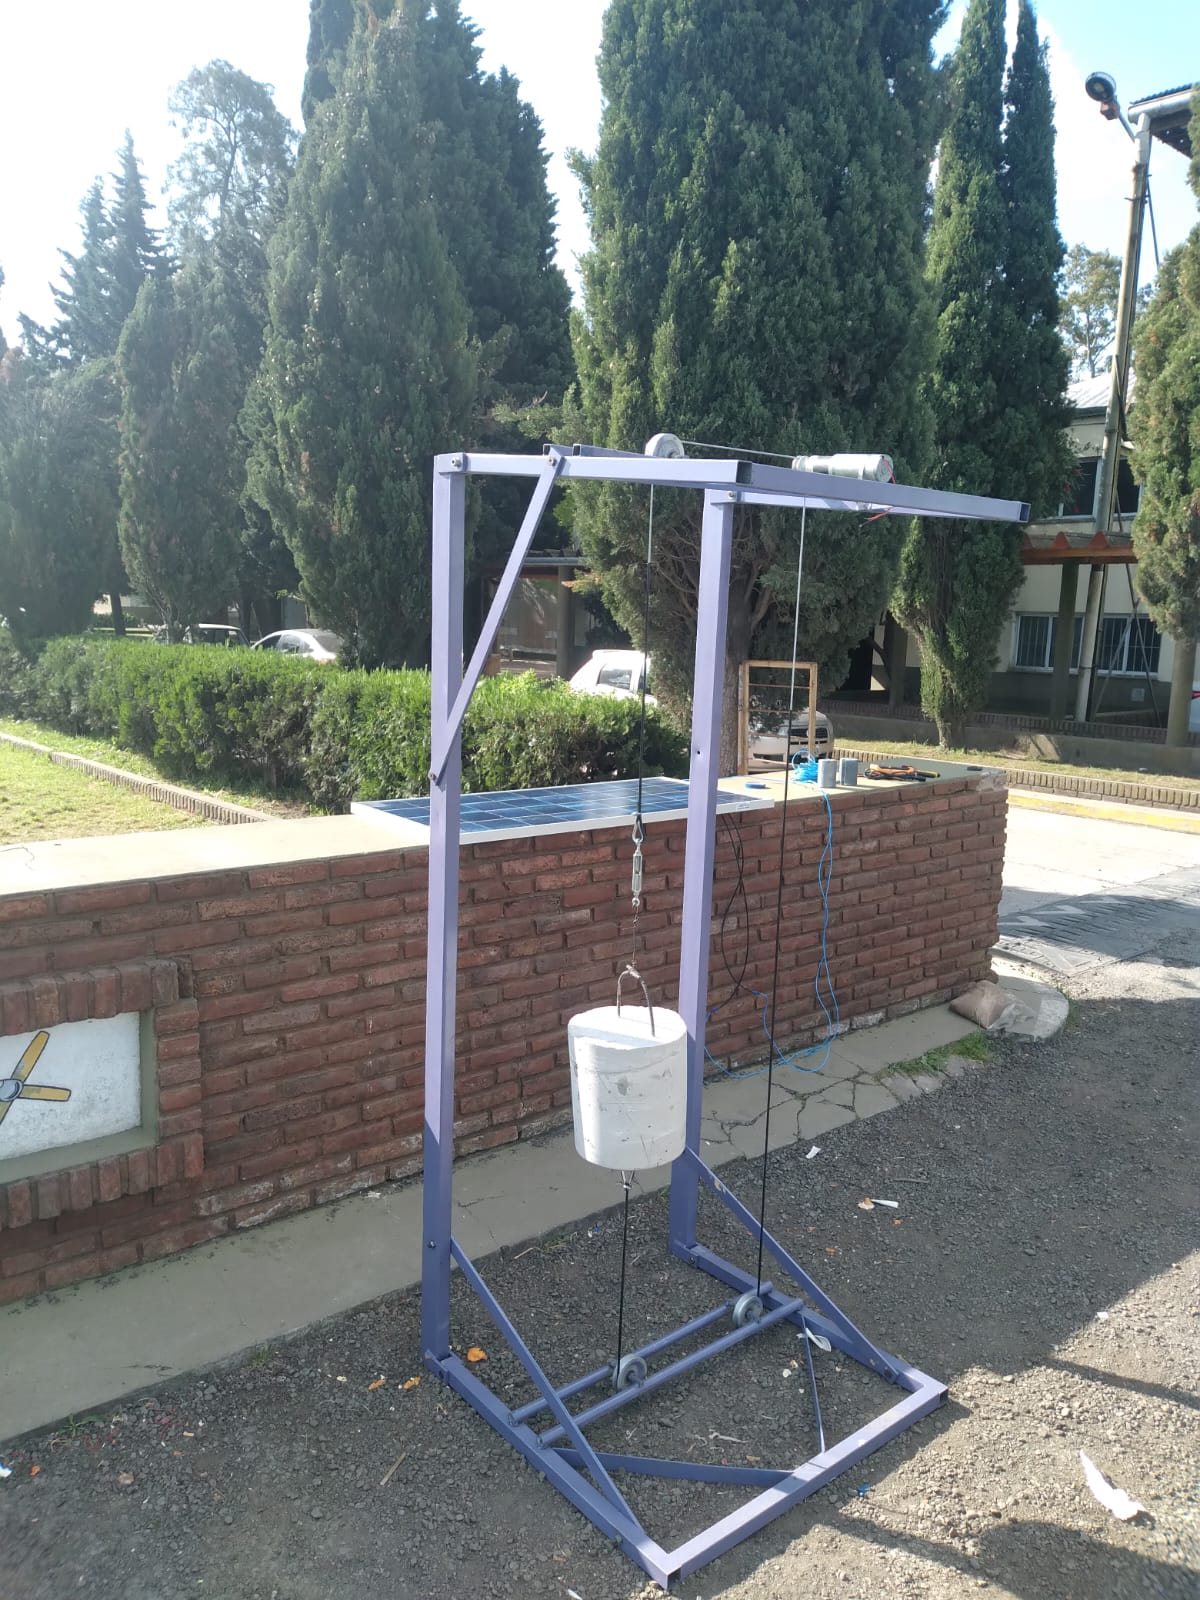
\includegraphics[width=\textwidth]{Estructura/Prototipo.png}
                    \caption{Prototipo de \textcolor{dark_violet}{\textbf{GraviCap}}}
                    \label{fig:e1.1}
                \end{subfigure}
                \begin{subfigure}[b]{0.3\textwidth}
                    \centering
                    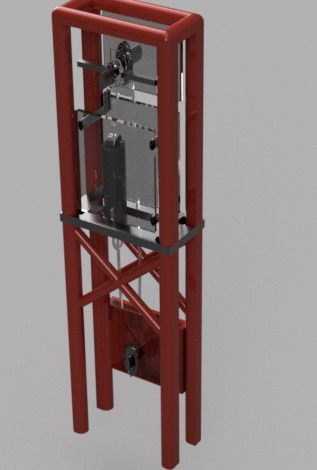
\includegraphics[width=\textwidth]{Estructura/Concepto.png}
                    \caption{Concepto de \textcolor{dark_violet}{\textbf{GraviCap}}}
                    \label{fig:e1.2}
                \end{subfigure}
                \caption{\textcolor{dark_violet}{\textbf{GraviCap}}}
                \label{fig:e1}
            \end{figure}
            
            Como alumnos, este proyecto es también una parte crucial de nuestro aprendizaje. Nos brinda la oportunidad de aplicar los conocimientos adquiridos en física, mecánica y sistemas eléctricos, además de desarrollar habilidades prácticas de diseño, ejecución y resolución de problemas. El prototipo a escala ha sido un paso esencial para comprender las implicaciones reales de implementar una batería gravitatoria, permitiéndonos abordar desafíos técnicos que probablemente también enfrentaríamos en una versión a mayor escala.\par
            El desarrollo de este prototipo nos ha proporcionado una visión clara de los beneficios y limitaciones de las baterías de gravedad, así como una base para futuras investigaciones y mejoras tecnológicas. Si bien nuestro prototipo no tiene la capacidad de almacenar grandes cantidades de energía, demuestra que esta tecnología es factible y escalable.\par
            Este enfoque educativo también nos motiva a pensar en soluciones reales para problemas energéticos actuales, como la necesidad de almacenamiento de energía renovable a gran escala, lo que refuerza la relevancia de nuestro trabajo en el contexto global de sostenibilidad y energía limpia.\par
\chapter{Cargador MPPT}
    
        \section{¿Qué es MPPT?}
        
            \textit{Maximum Power Point Tracking} es una técnica utilizada en cargadores para obtener la máxima potencia posible cuando las condiciones de alimentación son inestables.\par
            En los sistemas que utilizan, por ejemplo, energía solar la energía entregada depende de factores como la cantidad de luz, sombra, temperatura de los paneles, entre otras cosas. Cuando las condiciones son inestables, la impedancia característica que establece el punto de transferencia de potencia varía. Así, el sistema es optimizado cuando las condicones de la carga varían. A esto se le llama \textbf{MPP} (\textit{Maximum Power Point}) y al proceso \textbf{MPPT}\par
            
        \section{Principio de funcionamiento}
        
            \subsection{Convertidor DC-DC}
                Para convertir de un voltaje de continua de entrada mayor a uno menor, existen una infinidad de opciones. Se podría realizar un divisor resistivo, el cual disipa la potencia que no querramos, que sería poco eficiente. Para ocaciones en las que se busca conservar la máxima eficiencia posible con la mínima pérdida de potencia posible.\par
                Ahí es dónde entra el conversor Buck, o conversor reductor, que a la vez que reduce el voltaje de salida aumenta la corriente de salida, manteniendo constante la potencia. Es una clase de fuente switching, y provee una eficiencia muy alta, por encima de un 90\%. Además, controlando la señal de switching, podemos variar el voltaje de salida a voluntad.\par

                \begin{figure}[!ht]
                    \centering
                    \begin{subfigure}[b]{0.3\textwidth}
                        \centering
                        
\includegraphics[width=\textwidth]{MPPT/Buck.png}
                        \caption{Componentes del Conversor Buck}
                        \label{fig:m1.1}
                    \end{subfigure}
                    \begin{subfigure}[b]{0.3\textwidth}
                        \centering
                        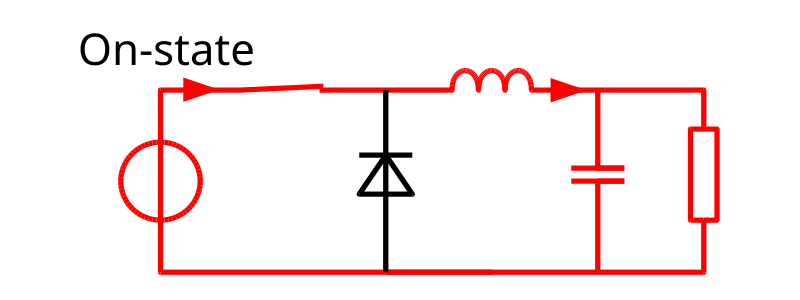
\includegraphics[width=\textwidth]{MPPT/Buck-On.png}
                        \caption{Estado On del Conversor Buck}
                        \label{fig:m1.2}
                    \end{subfigure}
                    \begin{subfigure}[b]{0.3\textwidth}
                        \centering
                        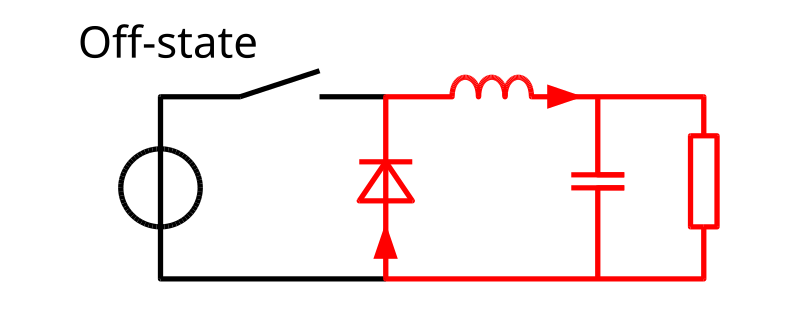
\includegraphics[width=\textwidth]{MPPT/Buck-Off.png}
                        \caption{Estado Off del conversor Buck.}
                        \label{fig:m1.3}
                    \end{subfigure}
                    \caption{Conversor Buck}
                    \label{fig:m1}
                \end{figure}

                Para entender este circuito, se debe hacer un análisis del estado transitorio del mismo en sus dos estados, On y Off. En principio, con el estado Off, la corriente en el circuito es nula. Cuando cambia al estado On, la corriente va empezar a subir y la bobina va a generar una caída de voltaje entre sus terminales. Esta caída de voltaje provoca que el voltaje resultante en la carga sea menor. A medida que pasa el tiempo, el índice de cambio de la corriente disminuye, y el voltaje en la bobina también disminuye, aumentando el voltaje en la carga. Durante este proceso, la bobina almacena energía en forma de campo magnético\par
                Cuando el interruptor de abre de vuelta (Off), la fuente de voltaje se remueve del circuito y la corriente disminuye. Esta corriente decreciente produce una caída de voltaje en la bobina (opuesto al generado en el estado On), y ahora la bobina se convierte en una fuente de corriente. La energía almacenada en el campo magnético de la bobina suporta el flujo de corriente por la carga. Esta corriente, que fluye mientras la fuente de voltaje está desconectada, cuando se suma a la corriente que fluye en el estado On, da como resultado una corriente de salida promedio mas grande que la que entrega la fuente de voltaje.\par

                \begin{figure} [!ht]
                    \centering
                    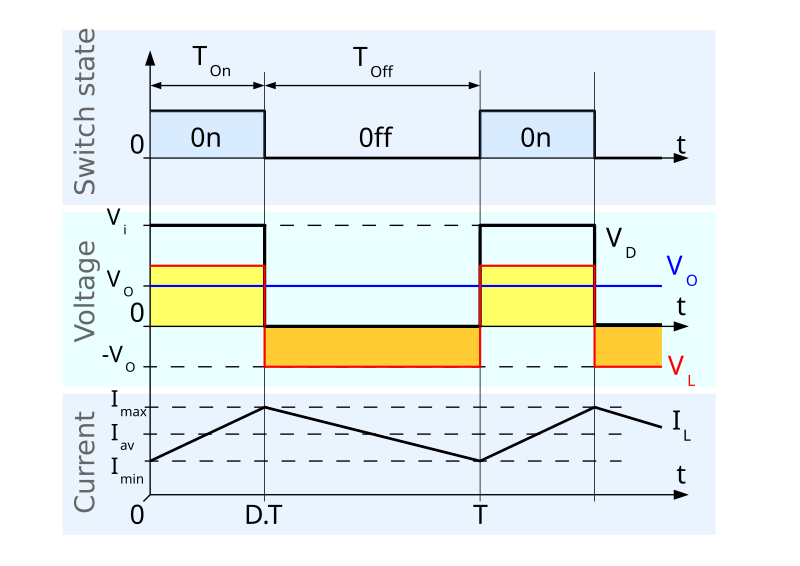
\includegraphics[width=0.6\linewidth]{MPPT/Gráfica.png}
                    \caption{Gráfica en el tiempo del comportamiento de las tensiones y corrientes de un convertidor buck.}
                    \label{fig:m1.4}
                \end{figure}
                
                Este aumento en la corriente promedio estaría compensando la reducción en el voltaje, manteniendo idealmente la potencia entregada en la carga. Si el switch se abre mientras la corriente sigue aumentando, entonces siempre va a haber una caída de tensión sobre la bobina, por lo tanto la carga siempre tendra menos voltaje que la entrada.\par

            \subsection{Sistema de Control}
                Si uno logra variar la frecuencia con la que ese switch se abre y se cierra, y al mismo tiempo medir la corriente y la tension recibida en la carga, se puede diseñar un sistema de control que, teniendo en cuenta esas variables, varíe esa frecuencia del interruptor con esas mediciones como realimentación, controlando una o la otra.\par
                El sistema de control que utilizamos es un control proporcional integral, o \textbf{PI}, siendo la aplicación de un control proporcional y uno integral al mismo tiempo.\par
                La parte proporcional de un control es el producto entre la señal de error ($e_{(t)}$) y la constante proporcional ($K_p$). Variando ($K_p$) se cambia la velocidad del control. Pero solo con un control proporcional se tiene error en régimen permanente, ya que este tipo de control requiere de error para entregar señal de control. La fórmula matemática que responde a esto es:\par
                \begin{equation}
                    P_{sal} = K_p \times e_{(t)}
                \end{equation}
                La parte integral del control actua cuando hay una desviación entre la variable y el punto de consigna, integrando esta desviación en el tiempo. El error es integrado, lo cual tiene la función de promediarlo o sumarlo por un período determinado, y luego se multiplica por una constante $K_i$. Elimina el error de estado estacionario, logrando seguimiento perfecto de la señal de referencia. La fórmula matemática que responde a esto es:\par
                \begin{equation}
                    I_{sal} = K_i \times \int e_{(t)} \ dt
                \end{equation}
                
        \section{Realización}
            \subsection{Esquemático}
                Se podrá encontrar el esquemático en el Apéndice A, que contiene los esquemáticos del proyecto.\par
            
            \subsection{Hardware}
                Para la realización de este cargador utilizamos una \textbf{RP2040 Zero}. Que luego se comunicará con el módulo de control para informar sobre los parámetros medidos.\par
                Para la medición de la corriente utilizamos un módulo \textbf{INA 219} que nos permite medir de forma precisa los parámetros de corriente.\par
                Para medir las tensiones tanto de entrada como de salida simplemente utilizamos divisores resistivos, los cuales nos devuelven voltajes proporcionales reducidos, tambien procesados por los otros dos ADCs de la RP2040 Zero. Para la conversion simplemente se tiene en cuenta la relacion de las resistencias.\par
                Para la alimentación del circuito se aprovecha el voltaje entregado por el cargador, donde conectamos una fuente stepdown que regula la tensión entregada por el cargador a 5V para la alimentación de la RP2040 Zero. Esto quiere decir que una vez que se conecta, el circuito ya se encuentra alimentado por energías renovables.\par
                En el circuito MPPT, la única diferencia con el teórico es el interruptor. Nuestro interruptor es un MOSFET canal P IRF4905, que resiste hasta 70A de corriente. Es necesaria la utilización de un MOSFET canal P porque la carga del mismo tiene que estar entre Drain y Masa, mientras que la carga de un canal N tiene que estar entre la alimentación y Source, algo que en nuestro diseño resultó inconveniente.\par
                Para conmutar este MOSFET con la Raspberry Pi Pico, no solo fue necesaria la utilización de un transistor NPN, sino tambien la de un circuito totem pole\par
                Un circuito totem pole consta de 2 transistores, un PNP y un NPN, uno arriba del otro, con sus bases interconectadas. Esto nos permite conmutar el MOSFET sin problemas, porque admite corrientes en ambos sentidos, tanto positivas como negativas. Esto es necesario porque un MOSFET necesita ambos sentidos de corrientes. Para entrar en estado de corte, necesita una corriente positiva en el Gate, y para volver al estado de saturación, por las características capacitivas del mismo, genera una corriente negativa.\par
                Para el cálculo del inductor, se realizó el siguiente procedimiento:\par
                Fijándose en la figura \ref{fig:m1.4}, el aumento de la corriente en la bobina queda:\par
                \begin{equation}
                    \frac{di_L(t)}{dt} = \frac{V_L(t)}{L} = \frac{V_i - V_o}{L}
                \end{equation}
                y análogamente el descenso de la corriente es:\par
                \begin{equation}
                    \frac{di_L(t)}{dt} = \frac{V_L(t)}{L} = \frac{-V_o}{L}
                \end{equation}
                Como toda la energía que se almacena en la bobina durante el primer estado se transfiere durante el segundo, la energía del inductor al final del periodo de conmutación ($T_S$) es igual en $t = 0$ y en $t = T_S$.\par
                Por lo tanto, la tensión media en la bobina ⟨$V_L$⟩ en régimen permanente es nula, es decir, existe una igualdad en las áreas.\par
                \begin{equation}
                    \langle V_L \rangle = \frac{1}{T_S}\int_{T_S} V_L dt = 0
                \end{equation}
                Aplicando la ecuación se obtiene:\par
                \begin{equation}
                    (V_i - V_o) \cdot DT_S - V_o \cdot (T_S - DT_S) = 0
                \end{equation}
                Donde $D$ es un número adimensional, entre 0 y 1, denominado ciclo de trabajo. Siendo que este no puede ser mayor a 1, se cumple $V_o \leq V_i$, por tanto solo se podrá reducir la tensión.\par
                \begin{equation}
                    V_o = D \cdot V_i
                    \label{eq:D}
                \end{equation}
                La corriente media que circula por la bobina, con un D del 10\% (peor condición posible):\par
                \begin{equation}
                    I_L > \frac{I_{Lmax}}{10} = 1A
                \end{equation}
                
                \begin{equation}
                    \frac{\Delta I_L}{2} < 1A \Rightarrow \Delta I_L < 2A
                \end{equation}\\
                Para calcular la bobina, se utiliza la siguiente fórmula:\par
                \begin{equation}
                    \frac{V_i - V_o}{L} \cdot D \cdot T_S < 2A
                \end{equation}\\
                Reemplazando D por la equivalencia obtenida en la fórmula \ref{eq:D}, queda:\par
                \begin{equation}
                    L \geq \frac{V_o(1-\frac{V_o}{V_i})\cdot T_S}{2}
                \end{equation}
                Siendo\par
                    \[V_i [24V-48V]\]
                    \[V_o [24V-28V]\]
                    \[T_S = 32 \cdot 10^{-6} S  = 32KHz\]\\
                El máximo de esta función queda definido por los máximos valores de tensión de entrada y tensión de salida, por lo tanto:\par
                \begin{equation}
                    L \geq \frac{28 \cdot (1-\frac{28}{48}) \cdot 32 \cdot 10^{-6}}{2}
                \end{equation}
                Entonces \[L \geq 99,5\mu H\]\\
                La bobina utilizada en el circuito posee un valor de \textbf{$83 \mu H$}, la cual cumple con la condición anterior.\\
                Para el cálculo del capacitor correspondiente, se realizó el siguiente procedimiento:\\
                Cálculo para el ripple del capacitor de un 1\%:\par
                \begin{equation}
                    \Delta V_o = 1\% \cdot 28V = 0,28V
                \end{equation}
                La fórmula utilizada para obtener el valor del capacitor es la siguiente:\\
                \begin{equation}
                    \Delta V_o = \frac{V_o \cdot (1-\frac{V_o}{V_i})}{8 \cdot L \cdot C \cdot F^2}
                \end{equation}\\
                Despejando, se obtiene:\\
                \begin{equation}
                    C \geq \frac{V_o \cdot  (1 - \frac{V_o}{V_i})}{8 \cdot L \cdot \Delta V_o \cdot F^2}
                \end{equation}\\
                Con los valores ya calculados, se reemplazan los parámetros:\\
                \begin{equation}
                    C \geq \frac{28V \cdot (1 - \frac{28V}{36V})}{8 \cdot 83 \mu H \cdot 32KHz^2}
                \end{equation}
                Entonces \[C \geq 27,13 \mu F\]\\
                Para evitar resonancias, se estima que la frecuencia de resonancia tiene que estar 10 veces por debajo de la frecuencia en la que se trabaja. Por esto:\\
                \begin{equation}
                    \frac{F_S}{10} = \frac{1}{\sqrt{L \cdot C}}
                \end{equation}
                Despejando, queda:\\
                \begin{equation}
                    C = \frac{10^2}{32KHz^2 \cdot 27,13 \mu H} \simeq 2713 \mu F
                \end{equation}\\
                Por lo tanto, en el circuito final se utilizó un capacitor de \textbf{$3300 \mu F$}

            \section{Software}
                El sistema MPPT fue programado íntegramente con el lenguaje C sobre la RP2040.\par
                El microcontrolador lee las señales del divisor de tensión que caerá sobre sus ADC y, mediante una lógica dependiente de la relación entre las resistencias del divisor de tensión, el código interpreta estas señales para saber el valor deseado (ya sea corriente o votaje).\par
                Ya sabiendo los valores que se tienen que medir, se compararán con los valores definidos para el cambio de lógica. Así se define en que modo de carga estará el MPPT. Por ejemplo, para el cambio entre BULK y ABSORTION, el voltaje de la batería deberá ser mayor al voltaje máximo definido del modo BULK.\par
                Cada modo tiene su propia lógica para manejar el PWM que regula la tensión y corriente que le llega a la batería. En el modo BULK, primero se calcula el error entre la medicion actual y la deseada, luego se ve si la corriente que le llega a la batería es mayor o menor a la deseada y en base a esto se controla el PWM proporcionalmente e integralmente tomando en cuenta el error, pasando previamente por un saturador, asegurándose que el valor del PWM no sea ni mayor a 100\% ni menor a 0\%.\par
                Para conocer más sobre todo esto, referirse al Anexo B, más específicamente el Listing \ref{Listing B.1}.
                
            \subsection{Resultado Final}
                \begin{figure}[H]
                    \centering
                    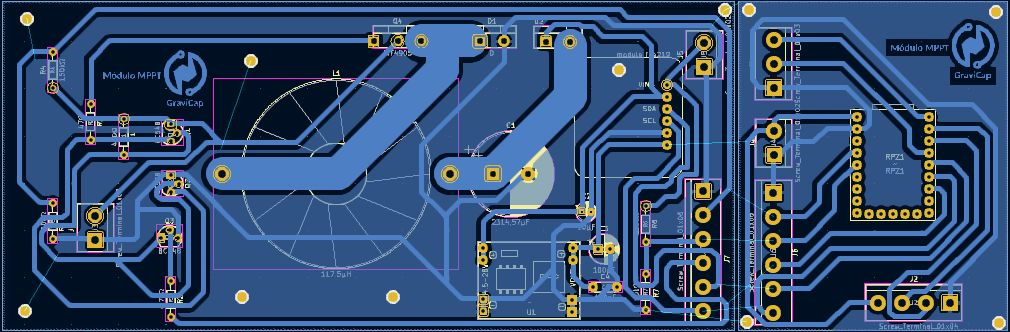
\includegraphics[width=0.8\linewidth]{MPPT/PCB - MPPT.png}
                    \caption{PCB del MPPT}
                    \label{fig:m5.1}
                \end{figure}
\chapter{Software}

    \section{Funcionamiento del Sistema de Control}
    
        \subsection{Introducción}
        
            El sistema de control del proyecto es el encargado de administrar los periodos de carga y descarga de la batería, optimizando su uso en función de los datos recogidos en tiempo real por los distintos sensores que lo integran, distintos datos en formato analógico de la batería, que son sensados para luego ser digitalizados y enviados a la aplicación móvil del usuario.\par
            Esta etapa forma el núcleo lógico del sistema, protagonizada por una RP2040-Zero, ejerce como nexo entre los componentes analógicos y nuestra aplicación.\par
            El microcontrolador se encuentra programado en C, un lenguaje que gracias a su bajo nivel, podrá ser ejecutado por el microcontrolador a una velocidad adecuada.\par
            
        \subsection{Datos obtenidos}
        
            Esta placa cuenta con 2 tipos de sensor principales, que trabajando en conjunto entregan los datos del funcionamiento en tiempo real de la batería y del sistema, información suficiente para continuar con su control.\par
            
            \subsubsection{Encoder Rotativo Incremental}
            
                Encargado de brindarle información al sistema sobre la posición y la velocidad angular, datos que utilizará el sistema para calcular la cantidad de vueltas y la dirección en la que rota el motor. Posee una gran precisión en sus respuestas por la cantidad de pulsos que envía por revolución. Nos permite calcular el porcentaje de carga de la batería, mientras nos brinda los datos para prevenir el funcionamiento errático del sistema.\par
                Para más información sobre este componente en concreto revisar el Apéndice C, y más específicamente la Figura \ref{encoder}.\par

                \subsubsubsection{Funcionamiento del Encoder}
                \label{fde}
                
                    El encoder basa su funcionamiento en dos señales digitales A y B, estas son generadas en cada pulso y están desfasadas 90° entre sí. Cuando el encoder está alimentado, comienza a enviar pulsos, mismos que variarán cuando el motor esté en movimiento. Para decodificar esta sucesión de pulsos, utilizamos la lectura en cuadratura. Este método basa su funcionamiento en la detección de cambios o transiciones entre las señales A y B.\par
                    Analizando dicha sucesión, este sistema busca detectar el momento en el que se complete un \textbf{ciclo} o \textbf{vuelta}, una sucesión de 4 estados en los que:\par
                    
                    \begin{itemize} [label=•]
                        \setlength{\itemindent}{1.5em}
                        
                        \item A sube (0 a 1)
                        \item B sube (0 a 1)
                        \item A sube (1 a 0)
                        \item B sube (1 a 0)
                    \end{itemize}
                    
                    Es importante observar que hacemos énfasis en el estado anterior de cada señal, ya que lo que realmente nos interesa es la transición entre un estado y otro.\par
                    Nuestro sistema utiliza un contador \texttt{\textbf{counter}} para llevar registro de las transiciones que efectúan las señales del encoder, este se incrementa a medida que se presentan las variaciones que nos interesan. A continuación, presento una serie de estados en los que observaremos el ciclo mencionado anteriormente y el uso del contador en él\par

                    \begin{table}[H]
                        \centering
                        \begin{tabular}{|c|c|c|c|c|c|c|}
                            \hline
                             N° & Estado Anterior A & Estado Anterior B & Estado Actual A & Estado Actual B & Acción & Contador\\
                             \hline
                             1 & 0 & 0 & 0 & 0 & - & -\\
                             \hline
                             2 & 0 & 0 & 1 & 0 & A sube & +1 (\texttt{\textbf{counter}})\\
                             \hline
                             3 & 1 & 0 & 1 & 0 & - & -\\
                             \hline
                             4 & 1 & 0 & 1 & 1 & B sube & -\\
                             \hline
                             5 & 1 & 1 & 0 & 1 & A baja & -1 (\texttt{\textbf{counter}})\\
                             \hline
                             6 & 0 & 1 & 0 & 0 & B baja & -\\
                             \hline
                        \end{tabular}
                        \caption{Tabla de Verdad para Encoder Rotativo en Cuadratura}
                        \label{tab:s1}
                        \end{table}
                        
                        Observamos que:\par
                        \begin{itemize} [label=•]
                            \setlength{\itemindent}{1.5em}
                            
                            \item Cuando ambos pulsos son iguales, no hay cambios en el \texttt{counter} (Estados 1 y 3).
                            \item El incremento del \texttt{counter} (\texttt{counter ++}) ocurre cuando A aumenta y A se mantiene (Estado 2).
                            \item La reducción del \texttt{counter} (\texttt{counter --}) ocurre cuando B aumenta y A se mantiene (Estado 4)
                            \item  Cuando cualquiera de las variables baja a 0 mientras la otra se mantiene, no hay cambios en el \texttt{counter} (Estados 5 y 6).
                        \end{itemize}
                        
                    El incremento en el counter implica giro en sentido horario, su reducción será giro en sentido antihorario.\par
                    Teniendo en cuenta la cantidad de pulsos que emite nuestro encoder por cada revolución, podremos\par

                \subsubsubsection{Datos obtenidos por el Encoder}
                    El encoder de nuestro sistema se encuentra conectado al eje del motor generador que mueve la carga de la batería. El encoder nos brinda información angular sobre la posición del eje del motor y las vueltas que realizó.\par
                    Conociendo la cantidad de vueltas que equivalen a un recorrido completo de la batería, podremos conocer el punto al que se encuentra el peso durante todo su funcionamiento.\par
                    Principalmente, buscamos evitar dos situaciones:\par
                    
                    \begin{itemize} [label=•]
                \setlength{\itemindent}{1.5em}
                        \item Si el peso se encuentra muy cerca del límite inferior, \textbf{NO} podrá descargarse la batería.
                        \item Si el peso está muy cerca del límite superior, el mismo \textbf{NO} podrá seguir subiendo con la carga de la batería.\par
                    \end{itemize}
                    
                    Estos factores son cruciales porque impiden un posible fallo mecánico de la batería, uno que podría derivar en fuertes daños al dispositivo, sus alrededores y seres circundantes.\par
                    Aparte de los riesgos potenciales que podemos prevenir, nos encontramos en la necesidad de controlar la carga y descarga de la batería, conocer el porcentaje de carga en el que se encuentra y asegurarnos de brindarle esta información al usuario. Con los datos que nos brinda el encoder podemos calcular el porcentaje de carga de la batería; ya que:\par
                    \begin{equation}
                        Porcentaje_{Carga} = \frac{\texttt{lap\_counter}}{\texttt{complete\_laps}} \times 100
                    \end{equation}
                    
                    Donde:\par
                    \begin{itemize} [label=•]
                \setlength{\itemindent}{1.5em}
                
                        \item \texttt{complete\_laps} es la cantidad de vueltas que necesita la batería para completar el recorrido.
                        \item \texttt{lap\_counter} es la cantidad de vueltas que realizó el motor, se actualiza constantemente, cuando realiza vueltas en sentido horario el contador aumenta, y cuando las realiza en sentido antihorario decrece.
                    \end{itemize}
                    
            \subsubsection{INA219}
                El sistema cuenta con 4 sensores INA219. Cada sensor se encuentra midiendo distintos parámetros, con la finalidad de asegurarle al sistema de control valores actualizados de corriente y tensión; de esta forma, el sistema podrá informar al usuario sobre sus acciones a nivel energético, mientras administra la carga y descarga de la batería de forma óptima en tiempo real.\par
                Para más información sobre este componente en concreto revisar el Apéndice C, y más específicamente la Figura \ref{ina219}.\par

                \subsubsubsection{Funcionamiento del INA219}
                    Estos sensores tienen un principio de funcionamiento muy simple, cuentan con una resistencia de shunt (una resistencia cuyo valor es muy bajo) conectada en serie a la carga.\par
                    El circuito obtiene la diferencia de potencial eléctrico entre sus terminales V+ y V- (donde se encuentra conectada la carga) y conoce el valor de la fuente de alimentación del circuito, por lo tanto podrá obtener el valor de la V de shunt.\par
                    
                        \begin{equation}
                            V_{Shunt} = V_{Total} - V_{Carga}
                        \end{equation}

                    El valor de la tensión de Shunt será muy bajo (suele ser menor a 50mV). El sensor lo que busca es obtener este valor para, utilizando la Ley de Ohm, obtener el valor de corriente.\par

                    \begin{equation}
                        I_{Shunt} = \frac{V_{Shunt}}{R_{Shunt}}
                    \end{equation}

                    Para hacer este cálculo, el valor de Vshunt tiene que estar en formato digital, por este motivo el módulo INA219 tiene su propio ADC integrado. Dentro de las configuraciones que solicitan los módulos encontramos los rangos de revolución del ADC interno. De acuerdo a la cantidad de bits que solicitemos, tendremos mayor o menor precisión en los resultados de las medidas; mientras más bits tendremos más precisión, pero también tomará más tiempo el proceso.\par

                    \begin{table}[H]
                        \centering
                        \begin{tabular}{|c|c|}
                        \hline
                            Resolución (bits) & Tiempo de Conversión\\
                        \hline
                             9 bits & 84 $\mu s$ \\
                        \hline
                            10 bits & 148 $\mu s$\\
                        \hline
                            11 bits & 276 $\mu s$\\
                        \hline
                            12 bits & 532 $\mu s$\\
                        \hline
                        \end{tabular}
                        \caption{Tabla de resolución del ADC}
                        \label{tab:s2}
                    \end{table}

                    Una señal tan pequeña (menor a 50mV) contará con muy poco porcentaje de resolución efectiva. La solución que nos propone el mismo módulo es amplificar la señal, dentro de los parámetros de configuración nos encontramos con 4 opciones de ganancia para la $V_{Shunt}$:\par

                    \begin{table}[H]
                        \centering
                        \begin{tabular}{|c|c|}
                        \hline
                            Ganancia & Máximo $V_{Shunt}$ medible\\
                        \hline
                             1x & ±320 mV \\
                        \hline
                            2x & ±160 mV\\
                        \hline
                            4x & ±80 mV\\
                        \hline
                            8x & ±40mV\\
                        \hline
                        \end{tabular}
                        \caption{Tabla de Ganancias}
                        \label{tab:s3}
                    \end{table}
                    
                    Cada valor de ganancia tiene un amplificador asociado, cada uno cuenta con sus propias características, su valor de ganancia y un valor máximo absoluto. Es importante asegurarnos de no exceder dicho valor porque causaría una saturación en la salida del amplificador, resultando en una pérdida de datos y una lectura incorrecta.\par
                    Una vez calculado el valor de corriente de shunt, podremos suponer que este es el mismo que circula por el resto de la rama, incluyendo a la carga.\par

                    \begin{equation}
                        I_{Shunt} = I_{Carga}
                    \end{equation}
                    
                    El valor de corriente se encuentra en formato digital y listo para ser enviado.\par
                    El módulo de INA219 cuenta con un puerto de comunicación i2c. Estos sensores permiten el uso en simultáneo de hasta 16 dispositivos INA219 conectados en el mismo puerto i2c. Dicha función es posible porque los datos enviados se encuentran encabezados por un byte de dirección, dato que se puede configurar desde los pines A1 y A0 de los módulos. Al conectar estos pines a distintos puntos, podremos obtener distintas direcciones, a continuación podemos observar las distintas posibilidades que nos ofrece.\par

                    \begin{table}[H]
                        \centering
                        \begin{tabular}{|c|c|c|}
                        \hline
                            \texttt{A1} & \texttt{A0} & \texttt{SLAVE ADDRESS}\\
                        \hline
                             \texttt{GND} & \texttt{GND} & \texttt{1000000}\\
                        \hline
                            \texttt{GND} & \texttt{Vs+} & \texttt{1000001}\\
                        \hline
                            \texttt{GND} & \texttt{SDA} & \texttt{1000010}\\
                        \hline
                            \texttt{GND} & \texttt{SLC} & \texttt{1000011}\\
                        \hline
                            \texttt{Vs+} & \texttt{GND} & \texttt{1000100}\\
                        \hline
                            \texttt{Vs+} & \texttt{Vs+} & \texttt{1000101}\\
                        \hline
                            \texttt{Vs+} & \texttt{SDA} & \texttt{1000110}\\
                        \hline
                            \texttt{Vs+} & \texttt{SLC} & \texttt{1000111}\\
                        \hline
                            \texttt{SDA} & \texttt{GND} & \texttt{1001000}\\
                        \hline
                            \texttt{SDA} & \texttt{Vs+} & \texttt{1001001}\\
                        \hline
                            \texttt{SDA} & \texttt{SDA} & \texttt{1001010}\\
                        \hline
                            \texttt{SDA} & \texttt{SLC} & \texttt{1001011}\\
                        \hline
                            \texttt{SLC} & \texttt{GND} & \texttt{1001100}\\
                        \hline
                            \texttt{SLC} & \texttt{Vs+} & \texttt{1001101}\\
                        \hline
                            \texttt{SLC} & \texttt{SDA} & \texttt{1001110}\\
                        \hline
                            \texttt{SLC} & \texttt{SLC} & \texttt{1001111}\\
                        \hline
                        \end{tabular}
                        \caption{Tabla I2C}
                        \label{tab:s4}
                    \end{table}
                    Para nuestro sistema, solo necesitamos 4 dispositivos, por lo tanto 4 direcciones.\par
                    \begin{table}[H]
                        \centering
                        \begin{tabular}{|c|c|c|c|}
                        \hline
                            \texttt{A1} & \texttt{A0} & \texttt{SLAVE ADDRESS} & \texttt{HEXADECIMAL VALUE}\\
                        \hline
                             \texttt{GND} & \texttt{GND} & \texttt{1000000} & \texttt{0x40}\\
                        \hline
                            \texttt{GND} & \texttt{Vs+} & \texttt{1000001} & \texttt{0x41}\\
                        \hline
                            \texttt{Vs+} & \texttt{GND} & \texttt{1000100} & \texttt{0x44}\\
                        \hline
                            \texttt{Vs+} & \texttt{Vs+} & \texttt{1000101} & \texttt{0x45}\\
                        \hline
                        \end{tabular}
                        \caption{Valores que usamos}
                        \label{tab:s5}
                    \end{table}
                    
                    Para configurar los registros de dirección de los módulos, estos cuentan con los pines A1 y A0. Por practicidad, cada uno tiene un pin que lo acompaña y que nos facilita su conexión con el pin de Vs+. Nos permite realizar un puente entre ambos pines (el pin An queda conectado a Vs+) o dejarlo como se encuentra de fábrica, sin ninguna conexión (el valor que toma An será el de GND). El módulo ofrece más configuraciones que implican la conexión de A1 y A0 con otros puertos, pero para mantener las conexiones simples decidimos obviarlos.\par
                    
                \subsubsubsection{Datos obtenidos por el INA219}
                    Como mencionamos previamente, contamos con 4 módulos medidores de corriente, cada uno conectado a un punto distinto de nuestro sistema para realizar las mediciones correspondientes. Los sensores están destinados a:\par

                \begin{itemize} [label=•]
                    \setlength{\itemindent}{1.5em}
                    
                    \item Consumo del usuario.
                    \item Entrega del módulo MPPT.
                    \item Consumo del motor de la batería durante la carga.
                    \item Entrega del panel solar, previo al módulo MPPT.
                \end{itemize}
                
                Cada sensor requiere una dirección para poder utilizar el puerto I2C, respectivamente:\par

                \begin{itemize} [label=•]
                    \setlength{\itemindent}{1.5em}
                    
                    \item \texttt{0x40}
                    \item \texttt{0x41}
                    \item \texttt{0x44}
                    \item \texttt{0x45}
                \end{itemize}
                
                En función de los datos obtenidos, el sistema los procesará. A continuación una breve descripción de la utilidad que nos dará cada uno:\par

                \begin{itemize} [label=•]
                    \setlength{\itemindent}{1.5em}
                    
                    \item \texttt{0x40} Consumo del usuario: A través de esta lectura, conocemos el consumo actual del usuario. Nos permite manejar la carga y descarga de la batería en tiempo real al compararlo con la entrega de energía del MPPT.
                    \item \texttt{0x41} Entrega del módulo MPPT: Esta será la energía que luego tendrá disponible el consumidor, por eso es crucial el dato para saber si la energía obtenida es suficiente o no para su uso.
                \end{itemize}
                
                Estos últimos dos datos son recolectados con una alta prioridad en el programa que controla al sistema, ya que son cruciales para el funcionamiento de la batería en sí.\par
                
                \begin{itemize} [label=•]
                    \setlength{\itemindent}{1.5em}
        
                    \item \texttt{0x44} Consumo del motor de la batería durante la carga: El consumo de la batería es equivalente al monto de energía que nuestra batería “guarda”. Nos parece importante que quien utiliza el sistema sea consciente de su consumo y la eficiencia de su producto.
                    \item \texttt{0x45} Entrega del panel solar, previo al módulo MPPT: Este dato nos otorga información sobre el funcionamiento del panel solar, que luego será modificada por el MPPT. Combinando estos dos datos, podremos brindarle al usuario datos sobre su obtención de energía.
                \end{itemize}
                
        \subsection{Funcionamiento de la Batería}
            Una vez obtenidos los datos, el microcontrolador puede comenzar a administrar la carga y descarga de la batería. El sistema contempla distintos escenarios posibles para decidir su próxima acción, optando entre:\par
            
            \begin{itemize} [label=•]
                \setlength{\itemindent}{1.5em}
                
                \item Si la corriente que entrega el panel solar es suficiente, entrega energía directa desde el panel solar (mientras considera un posible excedente en dicha entrega, evalúa la posibilidad de aprovecharlo para cargar la batería).
                \item Si la corriente no es suficiente, decide descargar la batería.
            \end{itemize}
            
            Previo a cada movimiento que desee realizar el sistema sobre la batería, utiliza los datos recolectados por el encoder para chequear el porcentaje de carga a la que se encuentra, bloqueando el movimiento si:\par
            
            \begin{itemize} [label=•]
                \setlength{\itemindent}{1.5em}
                
                \item La carga es menor al 20\%, la batería no se seguirá descargando.
                \item La carga es mayor al 80\%, no seguirá cargándose.
            \end{itemize}
            
            Por otro lado, si la corriente entregada por el panel solar no supera en exceso el valor de corriente que necesita el motor para cargar el peso, no se le dará inicio a la carga de la batería. Esto se debe a que cada vez que el motor es encendido, consume un pico de corriente inicial, un valor que supera de forma significativa al consumo de corriente nominal del mismo. Para evitar este exceso de consumo de forma repetitiva o continua evitamos el inicio de la carga cuando el excedente de energía es bajo.\par
        \section{Códigos de la etapa de control}
        
            \subsection{Introduccción}
                La etapa de control, conformada por una RP2040-Zero, es manejada por un código principal main.c, este utiliza en su totalidad las funciones desarrolladas en la librería \textcolor{dark_violet}{\textbf{GraviCap}}.\par
                El microcontrolador que elegimos tiene disponibilidad de dos núcleos. Para este sistema decidimos aprovechar ambos. Uno de los núcleos trabaja con FreeRTOS, un sistema de respuesta en tiempo real que ordena las funciones que realiza el programa en forma de “tareas”, asignándoles distintas prioridades a cada una para intercalar la ejecución de todas ellas de forma óptima.\par
                Para más información sobre este componente en concreto revisar el Apéndice C, y más específicamente la Figura \ref{rp2040}\par
            
            \subsection{Librería \textcolor{dark_violet}{\textbf{GraviCap}}}
                Para este sistema creamos la librería gravicap, está conformada por los archivos gravi.c y gravi.h. Entre ambos códigos declaran y desarrollan la totalidad de las funciones que derivan en el funcionamiento del sistema.\par
                En el archivo gravi.h creamos una estructura mediciones\_ina219.\par
                \lstinputlisting[language=C, firstline=19, lastline=27]{gravi.h}\par
                Esta contiene el nombre de cada sensor INA219, sus datos de configuración y variables que almacenan los datos medidos por ellos.\par
                En gravi.h podemos encontrar rambién declaradas las funciones antes mencionadas, desarrolladas luego en el archivo gravi.c:\par
                
                \subsubsection{void task\_init(void *params)}
                    Esta función contiene todas las inicializaciones de los distintos puertos (UART, I2C y GPIO), configura el funcionamiento de cada sensor INA219 y declara las \textit{queues} que serán utilizadas posteriormente. Al tratarse de la primera función que ejecuta el programa, para asegurar que el motor esté frenado al principio (que no cargue ni descargue la batería antes de realizar cualquier tipo de consulta sobre el estado de la carga), por eso luego de iniciar y configurar todo aquello que requerirá el programa, ejecuta la función de stop(), desarrollada posteriormente.\par

                \subsubsubsection{void status()}
                    Esta función es la que llamamos antes de ordenar cualquier movimiento en la batería para consultar si es posible realizarlo. Esta espera que el \texttt{core\_1} envíe el valor de \texttt{carga} para poder realizar su función. Una vez recibido, considera el porcentaje de carga y el valor mínimo crítico (\texttt{min\_critico}), un valor de porcentaje destinado a acotar superior e inferiormente el intervalo por el que se desplaza el peso de la batería, de esta forma, evitamos que se desplace por los extremos, donde podría suceder que:\par
                    \begin{enumerate}
                    \setlength{\itemindent}{1.5em}
                    
                        \item Se desperdicie energía al solicitar una carga (el consumo de un pico de arranque del motor) por un intervalo bajo de carga.
                        \item Un fallo mecánico del dispositivo al seguir forzando el movimiento (carga o descarga) en el límite del intervalo existente.
                    \end{enumerate}
                    La función trabaja con las variables \texttt{test\_up} (habilitará la carga de la batería) y \texttt{test\_down} (habilitará la descarga de la batería), ambas variables del tipo bool (únicamente valdrán 0 o 1). La función prevee 3 situaciones posibles:\par
                    \begin{enumerate}
                    \setlength{\itemindent}{1.5em}
                    
                        \item La carga se encuentra cerca del límite inferior, entonces no puede bajar más pero sí puede subir (\texttt{test\_up = 0} y \texttt{test\_down = 1})\par
                        \lstinputlisting[language=C, firstline=310, lastline=310]{gravi.c}
                        \item La carga se encuentra cerca del límite superior, entonces no puede subir más, pero sí bajar (\texttt{test\_up = 1} y \texttt{test\_down = 0})\par
                        \lstinputlisting[language=C, firstline=320, lastline=320]{gravi.c}
                        \item La carga se encuentra dentro del rango intermedio donde ambas opciones son viables (\texttt{test\_up = 0} y \texttt{test\_down = 0})\par
                        \lstinputlisting[language=C, firstline=315, lastline=315]{gravi.c}
                    \end{enumerate}
                    Observamos que, cuando las variables se encuentran en 0 dan dejan constancia de que es seguro realizar dicho movimiento, cuando están en 1 lo impedirán.\par
                    Si se presentara un error extraordinario donde la función no puede ingresar en ninguno de las condiciones (if) de la función, la excepción (else) les da valor 1 a las dos variables, impidiendo cualquier movimiento posible hasta corregir el error.\par

                \subsubsection{Funciones de lectura de sensores INA219}
                    Estas 4 funciones son las que recogen los datos de cada uno de los sensores, para luego almacenarlos en sus variables correspondientes, dejándolos a disposición para su uso en el resto de las funciones.\par
                    \begin{itemize} [label=•]
                        \setlength{\itemindent}{1.5em}
                        
                        \item \texttt{void task\_lectura\_sensor\_ina219\_0x40()}
                        \item \texttt{void task\_lectura\_sensor\_ina219\_0x41()}
                        \item \texttt{void task\_lectura\_sensor\_ina219\_0x44()}
                        \item \texttt{void task\_lectura\_sensor\_ina219\_0x45()}
                    \end{itemize}
                
                \subsubsection{void task\_consulta\_all(void *params)}
                    Esta función es la principal encargada de activar la carga y la descarga de la batería según la solicitud del usuario y la entrega de energía del MPPT. Para tomar esta decisión, utiliza los valores de las variables de “test” (\texttt{test\_up} y \texttt{test\_down}, mismas que modifica la función status()).\par
                    Para analizar la situación en la que se encuentra el sistema en general, depende totalmente de dos datos:\par
                    
                    \begin{itemize} [label=•]
                        \setlength{\itemindent}{1.5em}
                        
                        \item La medición de corriente del Ina219 0x40 aquel que recoge los datos de consumo del usuario
                        \item La medición de corriente del módulo Ina219 0x41, el que recoge los datos de entrega del MPPT
                    \end{itemize}
                    
                    La función inicia solicitando los datos de una \texttt{queue} o cola \texttt{queue\_ina219\_consulta\_all} que incluye los dos valores antes mencionados.\par
                    \lstinputlisting[language=C, firstline=233, lastline=233]{gravi.c}\par
                    Luego llama a la función \texttt{status()}. Esta esperará la llegada del valor de \texttt{carga} para actualizar los valores de las variables de testeo \texttt{test\_up} y \texttt{test\_down}.\par
                    Una vez actualizados, la función plantea 2 posibles escenarios al considerar los valores de corriente del consumidor (Ina219 0x40) y la entrega del MPPT (Ina219 0x41).\par
                    \begin{enumerate}
                    \setlength{\itemindent}{1.5em}
                    
                        \item Si el consumidor está solicitando más de lo que entrega el MPPT\par
                        \lstinputlisting[language=C, firstline=320, lastline=320]{gravi.c}
                        En este caso, el programa considera el valor de \texttt{test\_down}, valor que indicará si la batería tiene la carga suficiente como para ser descargada entregando energía almacenada al usuario.
                        Si este valor fuera positivo (\texttt{test\_down = 0})es posible descargar la bateŕía para obtener la energía almacenada, el sistema lo hará.\par
                        Si el valor fuera negativo (\texttt{test\_down = 1}) no es posible efectuar la descarga, entonces el sistema dependerá de la energía de la red eléctrica.\par
                        \item Si el consumidor está solicitando menos de los que entrega el MPPT\par
                        \lstinputlisting[language=C, firstline=320, lastline=320]{gravi.c}
                        En este caso la variable a considerar será la de \texttt{test\_up}, ya que, luego de asegurarnos de que el consumo de nuestro usuario está cubierto al 100\% por la energía entregada por el MPPT, evaluamos la posibilidad de que haya un sobrante de energía que pueda ser aprovechado en la posteridad por el usuario.\par
                        Dicha evaluación considera 2 opciones:\par
                        \begin{enumerate}
                        \setlength{\itemindent}{1.5em}
                        
                            \item La cantidad de energía generada es igual a la consumida, o el sobrante es muy bajo para ser utilizado en una carga de la batería\par
                            \lstinputlisting[language=C, firstline=320, lastline=320]{gravi.c}
                            En este caso el consumidor queda consumiendo 100\% de energía renovable, mientras la batería permanece estática.\par
                            \item La cantidad de energía generada es mucho mayor a la consumida, por lo tanto hay un sobrante energético.\par
                            \lstinputlisting[language=C, firstline=320, lastline=320]{gravi.c}
                            El consumidor estará consumiendo toda la energía que solicite desde la salida del módulo MPPT, mientras la batería es cargada con el sobrante de energía. Dicho sobrante será aprovechado luego.\par

                        \end{enumerate}
                    \end{enumerate}

                \subsubsection{void core\_1\_task()}
                    Al utilizar el segundo núcleo del microcontrolador (\texttt{core\_1}), requerimos declarar una función que contenga las funciones que realizará el mismo. En nuestro caso, el \texttt{core\_1} centra sus funciones en la lectura del Encoder. Este envía pulsos constantemente, mismos que hay que leer sin pausa alguna para asegurar la recepción efectiva de cada uno de sus estados. Si perdiéramos alguno de ellos, podría volverse erróneo el resultado causando algún fallo o defecto en el funcionamiento del dispositivo.
                    Como explicamos en el apartado \ref{fde}, la lectura de los datos del encoder depende de los datos que envían permanentemente dos pines, dos señales seriales desfasadas 90°. La función considera los valores actuales y anteriores de ambas variables, detecta las transiciones y los ciclos durante las distintas lecturas. Cuenta con una variable \texttt{counter} que almacena las transiciones y luego la considera para obtener el \texttt{lap\_counter}, la variable que almacena la cantidad de vueltas.\par
                    La función consta de un bucle infinito\par
                    
                    \lstinputlisting[language=C, firstline=267, lastline=267]{gravi.c}
                    
                    De esta forma aseguramos que la lectura sea constante. El motivo por el que decidimos usar el modo \texttt{multicore}, fue permitir, justamente, este bucle infinito. Si la recolección de datos del encoder fuera ejecutada por el mismo núcleo que contiene el resto de las funciones, podría ocurrir dos escenarios:\par
                    \begin{enumerate}
                    \setlength{\itemindent}{1.5em}
                    
                        \item El resto de las tareas nunca ocurrirían, porque el núcleo está constantemente ocupado recolectando pulsos del encoder.
                        \item La lectura del encoder es leída con huecos, volviéndose completamente errónea e inutilizable.
                    \end{enumerate}
                    
                    El intercambio de datos entre ambos núcleos es posible gracias a la función\par
                    \texttt{void multicore\_fifo\_push\_blocking(uint32\_t data);}\par
                    Esta función envía un entero de 32 bits sin signo desde un núcleo al otro por medio de la FIFO (First In, First Out) interna del RP2040.\par
                    Observamos este intercambio de datos en dos situaciones:\par

                    \begin{enumerate}
                    \setlength{\itemindent}{1.5em}
                    
                        \item Cuando el porcentaje de carga varió hasta un 15\% desde su última actualización en el core\_1\par
                        \lstinputlisting[language=C, firstline=287, lastline=287]{gravi.c}\par
                        \item Cada vez que es llamada la función de status(); contiene una cola que espera el valor de \texttt{carga}//monoespaciado// para configurar los datos de test con variables actualizadas en la inmediatez\par
                    \end{enumerate}

                \subsubsection{void carga\_motor()}
                    Esta función es la que llamamos cada vez que queremos iniciar la carga de la batería. Durante el funcionamiento del sistema, el motor varía entre 3 estados:\par
                    \begin{enumerate}
                        \setlength{\itemindent}{1.5em}
                        \item Carga
                        \item Descarga
                        \item Frenado (\textit{stop})
                    \end{enumerate}

                    Previo al inicio de la carga, debemos corroborar que el motor no se encuentre en alguno de los dos estados restantes, descarga o frenado. A través de una serie de consultas sobre el estado previo de los relés encargados de iniciar cada movimiento, podemos reconocer en qué estado se encuentran previamente, dato que consideraremos para acomodar las configuraciones del otro relé, y los leds asociados a cada estado.\par

            \subsubsection{void motor\_stop()}
                Para evitar una descarga inminente, si es que el motor no se encuentra alimentado para realizar una carga, debemos conectar sus dos terminales entre sí, frenando el motor de forma inmediata. Para que efectuar esta conexión, ambos relés deben estar encendidos.\par

            \subsubsection{int descarga\_motor()}
                Al realizar la descarga del motor, no podemos simplemente alimentarlo de forma inversa porque de esta forma no estaríamos cumpliendo con la premisa principal de “hacer uso de la energía potencial gravitatoria almacenada”, simplemente estaríamos moviendo una carga sin sentido.\par
                Para evitar que esto suceda, durante una descarga habitual encendemos el motor en sentido inverso por un lapso de tiempo muy reducido, venciendo la fricción estática inicial de la carga mientras comienza a moverse.\par
                Teóricamente, el movimiento sostenido en el tiempo por la inercia que genera el peso de la carga, debería ser suficiente para evitar pausas en la descarga, pero esto puede fallar por pequeñas variaciones en el entorno que modifiquen el funcionamiento de la batería, podría tratarse de cambios en la temperatura, en la tensión de los cables de la batería, la densidad del aire, la flexión de los materiales u otros, presentándose pausas sin antes haber activado la pausa o la carga del motor.\par
                Si la descarga se detiene por cualquiera de estos factores, nuevamente le daremos un pulso al motor en sentido inverso para volver a tratar de vencer la fricción estática, acción que se repetirá hasta que acabe la solicitud de descarga por parte del sistema.\par
                Esta función es la encargada de mantener este estado de descarga venciendo las adversidades que pudieran presentarse en el entorno.\par

            \subsubsection{void actualizar\_leds(float porcentaje\_carga)}
                Para mantener el grado de carga de la batería explícito en un tablero que la acompaña, agregamos una serie de leds que representan un “cargador”, variando la cantidad que se encenderán a cada instante según el valor más reciente obtenido de la carga (cada led del tablero tiene distintos colores en función de la carga que representan, variando entre azul y rojo, para mantener la estética y practicidad en la lectura de este tablero).\par
                En un principio, la función solicita el valor de \texttt{porcentaje\_carga} (variable del tipo float), el mismo le será entregado como parámetro con el valor de carga actualizado. Esta función tiene como objetivo ser llamada durante la ejecución de \texttt{status()}, misma función que nos asegura el valor reciente de carga al solicitarlo al \texttt{core\_1} en sus primeras líneas.\par
                Considerando que \texttt{actualizar\_leds} se encuentra llamada en \texttt{status()}, misma función utilizada en \texttt{task\_consulta\_all}, aseguramos que la actualización de los leds se ejecute con la misma frecuencia que esta última tarea, una que cuenta con prioridad 3, valor que nos asegura que se repetirá con mucha frecuencia mientras funcione el sistema.\par

                \subsubsection{void prepare\_char\_uart(char *ubicacion, mediciones\_ina219 *medicion, size\_t ubicacion\_size, float porcentaje\_carga)}
                    Para enviar los distintos datos recolectados por los sensores al usuario, es necesario incluirlos a todos ellos en distintas cadenas de texto listas para ser transportadas por el puerto serial. Esta función es la encargada de crearlas.\par
                    Para realizar esta conversión, utiliza la función de C \texttt{snprint}, esta formatea cadenas de texto y las almacena en una cadena preexistente.\par
                    Sintaxis de la función: \texttt{int snprintf(char *buffer, size\_t buf\_size, const char *format, ...);}
                    Al principio del programa fueron declaradas 4, destinadas a contener los valores medidos de cada INA219.\par

                    \lstinputlisting[language=C, firstline=38, lastline=41]{gravi.c}\par
                    
                    El tamaño de cada una está especificado en:\par

                    \lstinputlisting[language=C, firstline=19, lastline=19]{gravi.c}\par
                    
                    De esta forma se encuentra con fácil acceso para ser modificado siempre que se requiera. Consideramos que las 4 cadenas tendrán tamaños iguales, todas contendrán el mismo tipo de dato.\par
                    La función solicita 4 parámetros:\par
                    \begin{enumerate}
                    \setlength{\itemindent}{1.5em}
                        
                        \item \texttt{char *ubicacion}: Refiere a la cadena donde se escribirán los datos luego especificados. Utilizamos las 4 cadenas mencionadas previamente.
                        \item \texttt{mediciones\_ina219 *medicion}: Se trata de la variable del tipo \texttt{mediciones\_ina219}, contenida localmente en una variable llamada \texttt{medicion}.
                        \item \texttt{size\_t ubicacion\_size}: Es el tamaño que tendrá la cadena en la que se almacena el resultado de esta operación. En nuestro caso, todas las cadenas tienen el tamaño previamente definido como \texttt{CHAR\_UART}.
                        \item \texttt{float porcentaje\_carga}: Es la variable definida localmente como \texttt{porcentaje\_carga}, pero la utilizamos para solicitar el valor de \texttt{carga}
                    \end{enumerate}
                    
                    Utilizando estos datos, la función genera una cadena del tipo JSON.\par

                    \lstinputlisting[language=C, firstline=330, lastline=330]{gravi.c}\par
                    
                    Donde podemos apreciar especificados los 5 valores destinados al servidor web.\par

                \subsubsection{void send\_uart()}
                    Esta función se encarga de preparar las cadenas de texto de cada sensor INA219, para hacerlo llama a la función \texttt{prepare\_char\_uart(char *ubicacion, mediciones\_ina219 *medicion, size\_t ubicacion\_size, float porcentaje\_carga)} cuatro veces (una por sensor), especificando entre sus parámetros los datos propios de cada sensor y sus cadenas asociadas.\par
                    Para efectuar estas tareas con los datos necesarios obtenidos y actuales, tiene una \texttt{queue queue\_ina219\_send\_uart }asociada.\par

                    \lstinputlisting[language=C, firstline=341, lastline=341]{gravi.c}\par                    
                    
                    Esta espera la recolección de los datos de los 4 sensores INA219, datos que se guardan en al \texttt{queue} al final de cada función de lectura de los mismos.\par
                    Luego de rellenar las 4 cadenas de texto, envía una por una por el puerto \texttt{UART1} utilizando la función \texttt{uart\_puts}\par
                    Sintaxis de la función: \texttt{void uart\_puts(uart\_inst\_t *uart, const char *s);}
                    
            \subsection{Programa Principal}
                \subsubsection{Introducción}
                    El programa principal, main.c, es el encargado de\par
                    El código principal trabaja delegando tareas a sus dos núcleos:\par
                \subsubsection{Uso de FreeRTOS}
                    Como mencionamos anteriormente, nuestro sistema requiere el manejo de datos y tareas en tiempo real, es por esto que optamos por la utilización del sistema \textbf{FreeRTOS}. Este requiere una sintaxis particular y un formato que difiere del utilizado habitualmente por los códigos \textbf{BareMetal}.\par
                    Su característica principal, es la utilización de tareas en la ejecución del programa, las mismas deben estar declaradas en el programa de ejecución principal o main.c. En su declaración, cada una solicita una serie de argumentos o parámetros especificados a continuación:\par

                    \lstinputlisting[lenguage=C]{adicional.c}
                    
                    Aquí un ejemplo de una de las tareas declaradas en este programa:\par
                    \lstinputlisting[language=C, firstline=67, lastline=73]{maino.c}\par

                    Uno de los parámetros que más vale la pena destacar es: \texttt{UBaseType\_t uxPriority}\par
                    En nuestro ejemplo:\par
                    \lstinputlisting[language=C, firstline=71, lastline=71]{maino.c}\par
                    Se trata del parámetro que le asigna distintas prioridades a las tareas.\par
                    Al utilizar FreeRTOS, no observamos el desarrollo de un programa habitual de BareMetal donde el código se ejecuta línea por línea hasta finalizar el archivo, en este caso ponemos en práctica el concepto de “Tarea” o \textit{Task}, conceptos propios de FreeRTOS.\par
                    Definición: Una tarea es “una serie de instrucciones que se ejecutará de acuerdo a su orden de prioridad hasta completarse, o hasta que presente una interrupción”.\par
                    \textbf{¿A qué nos referimos con esto?}\par

                    Nos interesa analizar dos conceptos centrales:\par
                    \begin{itemize} [label=•]
                        \setlength{\itemindent}{1.5em}
                        \item Orden de prioridad: Es uno de los parámetros que asignamos al momento de crear la tarea, como vimos previamente.\par
                        A la hora de ejecutar tareas, el programa empezará por aquellas que cuenten con la prioridad más alta, cuando abandone esta misma, irá por la siguiente con este mismo nivel de prioridad, si no lo hubiera baja un escalón y continúa por el siguiente nivel.\par
                        \item Interrupción: Con la finalidad de no perder tiempo en actividades vacías, el sistema de FreeRTOS nos permite realizar una interrupción en una tarea para reanudarla luego. Se ve así:\par
                        \lstinputlisting[language=C, firstline=170, lastline=170]{gravi.c}\par
                        En este caso, solicito una interrupción de 1000 Tiks, una medida de tiempo que configuré previamente.\par
                        La función de una tarea es ejecutada hasta que aparece la línea de interrupción; en este caso, el programa esperará 1000 tiks y volverá a reanudarla. Esto puede ser útil cuando la tarea solicita un dato o parámetro de otro dispositivo o similar, nos encontramos con “tiempo muerto” hasta que llegue la información. Para no desaprovecharlo, el código ejecuta otra tarea hasta que acaba el tiempo de Delay.\par
                        \end{itemize}
                    
                    Nuestro sistema basa su funcionamiento en 7 tareas.\par
                    Cada tarea tiene un nivel de prioridad designado, a continuación una tabla con el orden que les fue asignado.\par
                    
                        \begin{table}[H]
                            \centering
                            \begin{tabular}{|c|c|}
                            \hline
                                Tarea & Prioridad\\
                            \hline
                                task\_init & tskIDLE\_PRIORITY + 6UL (6) \\
                            \hline
                                task\_lectura\_sensor\_ina219\_0x40 & tskIDLE\_PRIORITY + 5UL (5)\\
                            \hline
                                task\_lectura\_sensor\_ina219\_0x41 & tskIDLE\_PRIORITY + 5UL (5)\\
                            \hline
                                task\_cons1ulta\_all & tskIDLE\_PRIORITY + 3UL (3) \\
                            \hline
                                1task\_lectura\_sensor\_ina219\_0x44 & tskIDLE\_PRIORITY + 2UL (2)\\
                            \hline
                                task\_lectura\_sensor\_ina219\_0x45 & tskIDLE\_PRIORITY + 2UL (2)\\
                            \hline
                                task\_send\_uart & tskIDLE\_PRIORITY + 1UL (1)\\
                            \hline
                            \end{tabular}
                            \caption{Tabla de Prioridades}
                            \label{tab:6}
                        \end{table}
                        
                    Mientras mayor sea el número de tskIDLE\_PRIORITY, mayor será la prioridad de la tarea.\par
                    En el caso de nuestro sistema, con 5 niveles de prioridad, dejando en primer lugar la función\par
                    \lstinputlisting[language=C, firstline=28, lastline=28]{maino.c}\par
                    
                    Es importante que esta función tenga la prioridad más alta para aseg1urar que se ejecute al principio del código sin excepciones, ya que contiene las distintas inicializaciones y configuraciones de pines, puertos y sensores. Esta tarea contiene una línea especial al final de la función, una que la elimina de la memoria luego de su finalización\par
                    \lstinputlisting[language=C, firstline=170, lastline=170]{gravi.c}\par
                    
                    De esta forma ahorramos memoria, sin sacrificar ningún dato de relevancia.\par
                    Podemos observar entre la designación de funciones listada en el archivo gravi.h, como aquellas que están destinadas a ser ejecutadas en una tarea, reciben un nombre encabezado por task\_ seguido de un título que hace referencia al uso que le daremos a esa función. Se trata de una convención utilizada en los nombres de las funciones de este estilo.\par
                    Revisando estas mismas tareas, esta vez en el archivo gravi.c donde se encuentran desarrolladas todas las funciones del programa, observamos como todas las tareas están compuestas por un bucle infinito (generalmente un \texttt{while(true)}). Esto se debe a que, por su naturaleza, las tareas no cuentan con principio o final, simplemente son listados de ejecuciones que deben repetirse de forma indefinida.\par
                    Para poder utilizar todas las funciones desde el archivo main.c sin la necesidad de declararlas allí, entre las primeras líneas de este archivo nos aseguramos de incluir los dos documentos que conforman la librería gravicap, donde previamente declaramos funciones y demás.\par
                    \lstinputlisting[language=C, firstline=2, lastline=3]{maino.c}\par
                
                \subsubsection{Uso del Multicore}
                    Los microcontroladores cuentan con uno o varios núcleos generalmente. Cada núcleo es una unidad de procesamiento independiente, cuenta con su propia unidad de procesamiento ALU (unidad aritmético-lógica) y su propio conjunto de registros.\par
                    Cada tarea que ordenamos realizar a nuestro microcontrolador, ocupa uno de sus núcleos por fracciones de segundo hasta acabar con dicha ejecución, sin permitir que otra función ocurra en simultáneo.\par
                    Aún administrando de forma inteligente el modo en el que nuestro microcontrolador ejecuta todas sus tareas, seguimos encontrándonos con una problemática a la hora de intentar ejecutar varias funciones a la vez.\par
                    En nuestro sistema utilizamos un Encoder, componente que entrega datos de forma constante a través de sus dos terminales de salida. Constantemente debemos leer los pulsos que envía y procesarlos, para asegurar que la lectura sea correcta.\par 
	                Uno de los núcleos del microcontrolador (core\_0) se encuentra constantemente ejecutando las tareas de FreeRTOS, mientras que al 2do núcleo (core\_1) le asignamos una única tarea, la lectura del encoder.
                    Para poder utilizar este 2do núcleo, tuvimos que iniciar las funciones del multicore en el main.c.\par
                    \lstinputlisting[language=C, firstline=25, lastline=25]{maino.c}\par
	                Donde iniciamos el multicore solicitando la ejecución de la tarea core\_1\_task en nuestro caso. Esta tarea, nuevamente está conformada por un bucle infinito, y tiene como único objetivo la lectura y procesamiento de datos del Encoder.\par
	                Teniendo en cuenta que cada núcleo cuenta con su propio conjunto de registros, al querer solicitar datos del núcleo sobre el que no estamos trabajando, nos encontramos con otra problemática.\par
	                FreeRTOS nos otorga una solución, la implementación de colas.\par
                    Al hablar de colas, interviene la elección de un “Método de gestión de cargas”. Se trata de las técnicas utilizadas en estructuras de datos al comenzar a utilizar la teoría de colas. Podemos encontrarnos con dos tipos de colas; estas difieren entre sí por el orden de llegada de datos, y su posterior orden de lectura:\par
                    \begin{itemize} [label=•]
                        \setlength{\itemindent}{1.5em}
                        \item FIFO (First-In, First-Out): Son colas cuyos valores de entrada son procesados en el mismo orden en el que fueron agregados.
                        \item LIFO (Last-In, First-Out). Son colas cuyo comportamiento responde a la lógica del “último elemento que ingresa es el primero en salir”.
                    \end{itemize}

                    \begin{figure}[H]
                        \centering
                        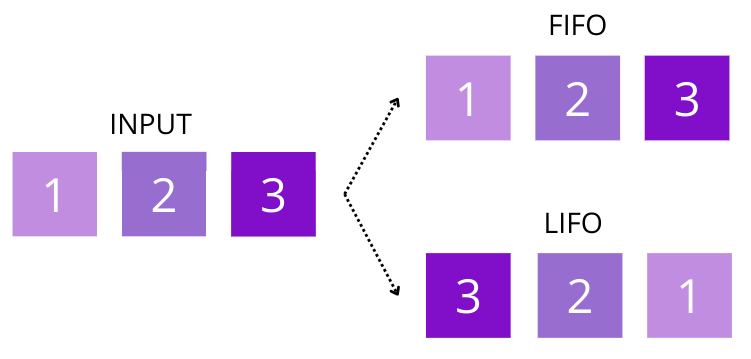
\includegraphics[width=0.5\linewidth]{Software/FIFO.png}
                        \caption{Cómo funciona FIFO y LIFO}
                        \label{fig:s1}
                    \end{figure}

                    En  nuestro programa, utilizamos colas FIFO para interconectar ambos núcleos, declarando un acceso directo a la entrada de la cola desde el \texttt{core\_0}, por ejemplo, en conjunto con otro acceso a la salida de dicha cola en el \texttt{core\_1}. No hay superposición entre los registros de ambos núcleos, por lo tanto puede funcionar de forma correcta.\par
	                Las colas FIFO las podemos utilizar desde nuestro programa aprovechando las funciones:\par
                    \texttt{void multicore\_fifo\_push\_blocking(uint32\_t data);}\par
                    Esta función es la que agrega un parámetro de formato (uint32\_t data) a la cola.\par
                    \texttt{uint32\_t multicore\_fifo\_pop\_blocking();}\par
                    Esta función es la que luego lo recogerá, para almacenarlo en una variable del mismo tipo.\par

%// void multicore_fifo_push_blocking(uint32_t data);
	%Esta función es la que agrega un parámetro de formato (uint32_t data) a la cola.
%// uint32_t multicore_fifo_pop_blocking();
%Esta función es la que luego lo recogerá, para almacenarlo en una variable del mismo tipo.

                %\subsubsection{Core0}
                    %Este núcleo trabaja con el sistema en tiempo real FreeRTOS, un sistema basado en tareas y en la interrupción/continuación de las mismas para asegurar un empleo óptimo de los recursos del microcontrolador.\par
                    %Cada tarea cuenta con un nivel de importancia o \textbf{prioridad}.\par
                    
                %\subsubsection{Core1}
                    %Este segundo núcleo es el encargado de recibir los datos del Encoder. Al tratarse de un componente que (durante la carga o descarga del motor) envía pulsos que habrá que leer y procesar en tiempo real, debimos administrar su lectura por separado.\par
                
        \section{Desarrollo del Servidor Web}
            
            \subsection{Módulo ESP8266-01}
                Se trata de un módulo wifi de la familia ESP, se encarga de generar un servidor web, mismo del que la aplicación móvil luego obtendrá los datos para el usuario.\par
                Para más información sobre este componente en concreto revisar el Apéndice C, y más específicamente la Figura \ref{esp8266}\par
            
            \subsection{Lógica}
                El sistema de control envía los datos recogidos cada una cierta cantidad de tiempo por medio de un canal de comunicación tipo UART a la ESP8266.\par
\chapter{Hardware}
    
        \section{Introdución}
            El hardware de la Etapa de Control en el sistema \textcolor{dark_violet}{\textbf{GraviCap}} es crucial para la gestión precisa de la energía y el control del movimiento del peso. Esta etapa permite la correcta operación de los motores, sensores y actuadores, asegurando un funcionamiento eficiente del sistema de almacenamiento y conversión de energía. El diseño de este hardware se basa en la implementación de transistores y controladores que trabajan en conjunto para optimizar el flujo de energía y garantizar una operación estable.\par

        \section{Indicadores LED}
            \subsection{Introducción}
                El sistema de control de GraviCap incluye un conjunto de LEDs que proporcionan información visual sobre el estado del sistema y el nivel de carga de la batería. Los LEDs de la derecha indican el estado operativo del sistema, mientras que los LEDs de la izquierda muestran el porcentaje de carga de la batería. Los LEDs están dispuestos para facilitar el monitoreo y permitir una comprensión rápida del estado del sistema.\par
                
            \subsection{LEDs de la Derecha}
                Los LEDs ubicados a la derecha del sistema reflejan el estado general de operación:
                \begin{itemize} [label=•]
                    \setlength{\itemindent}{1.5em}
                    
                    \item Blanco: Indica que el sistema está encendido (ON).
                    \item Azul: Señala que el sistema está en modo de carga, es decir, la batería está recibiendo energía.
                    \item Rojo: Indica que el sistema está en modo de descarga, es decir, la energía almacenada en la batería está siendo utilizada.
                \end{itemize}
                Estos LEDs permiten monitorear el estado activo del sistema de forma clara, mostrando cuándo está operando, cargando o descargando energía.\par
                
            \subsection{LEDs de la Izquierda}
                Los LEDs de la izquierda muestran el porcentaje de carga de la batería, ordenados de arriba hacia abajo según el nivel de carga:\par
                \begin{itemize} [label=•]
                    \setlength{\itemindent}{1.5em}
                    
                    \item Azul: Indica que la batería está al máximo nivel de carga.
                    \item Verde: Señala que la batería está casi completamente cargada.
                    \item Verde (intermedio): Representa que la batería tiene un porcentaje de carga por encima de la mitad.
                    \item Amarillo: Indica que la batería está a la mitad de su capacidad.
                    \item Amarillo (inferior): Indica que la batería está en un nivel de carga inicial.
                    \item Rojo: Señala que la batería está en un estado de carga nulo, es decir, se ha descargado completamente o está cerca de agotarse.
                \end{itemize}
                
                 Este orden secuencial de los LEDs de la izquierda proporciona una visualización rápida del estado de carga de la batería, permitiendo a los usuarios evaluar en qué punto del ciclo de carga o descarga se encuentra la batería con solo un vistazo.\par

        \section{Sistema de Conmutación}
        
            \subsection{Introducción}
                El sistema de conmutación en la Etapa de Control de \textcolor{dark_violet}{\textbf{GraviCap}} se encarga de gestionar el encendido y apagado del motor que controla la masa gravitatoria. Para lograr esto de manera eficiente, se utilizan relés que permiten la conmutación del motor, y estos relés son controlados por transistores BJT. Este sistema garantiza que la conmutación de las corrientes de alto voltaje sea segura y precisa.\par
                
            \subsection{Funcionamiento del Sistema de Conmutación}
                El sistema de conmutación opera mediante un esquema de control en dos etapas. Primero, los transistores BJT actúan como interruptores que controlan la activación de los relés. Estos relés, a su vez, son responsables de conmutar las corrientes de mayor potencia necesarias para el funcionamiento del motor de elevación de la masa.\par
                \begin{itemize} [label=•]
                    \setlength{\itemindent}{1.5em}
                    
                    \item Conmutación con relés: Los relés se utilizan para abrir y cerrar los circuitos de alta corriente que alimentan al motor. Cuando se recibe una señal de control desde el microcontrolador, los BJT se activan, lo que a su vez energiza los relés y permite el paso de corriente hacia el motor.
                    \item Control preciso: El uso de transistores BJT para conmutar los relés permite que el microcontrolador tenga un control preciso sobre cuándo activar o desactivar el motor, asegurando que la operación de carga y descarga se realice en los momentos adecuados.
                \end{itemize}
                
            \subsection{Eficiencia del Sistema de Conmutación}
                El uso de relés para la conmutación del motor, en combinación con los BJT, proporciona un equilibrio entre eficiencia y seguridad. Los relés son ideales para manejar corrientes más altas, mientras que los BJT se encargan de conmutar las señales de control de baja potencia que provienen del microcontrolador.

                \begin{itemize} [label=•]
                    \setlength{\itemindent}{1.5em}
                    
                    \item Relés de alta capacidad: Los relés seleccionados para el sistema pueden manejar las corrientes y voltajes necesarios para operar el motor, asegurando una conmutación confiable sin generar excesivo calor o desgaste en el circuito.
                    \item Conmutación controlada por BJT: Los transistores BJT permiten que la conmutación de los relés sea precisa, ya que estos se activan con señales de baja potencia desde el microcontrolador, lo que garantiza un control eficiente sin necesidad de grandes corrientes para el accionamiento directo de los relés.
                \end{itemize}
                
            \subsection{Protección del Sistema de Conmutación}
                El sistema de conmutación incluye mecanismos de protección que garantizan la seguridad tanto de los relés como de los transistores BJT. Estos mecanismos aseguran que el sistema funcione de manera estable bajo diversas condiciones de carga.\par
                Se han implementado protecciones para evitar que corrientes excesivas dañen los relés o los transistores BJT. Estas protecciones son cruciales para prevenir fallos en el sistema, especialmente durante la conmutación de grandes cargas.\par
            
        \section{Resultado Final}
            \begin{figure}[H]
                    \centering
                    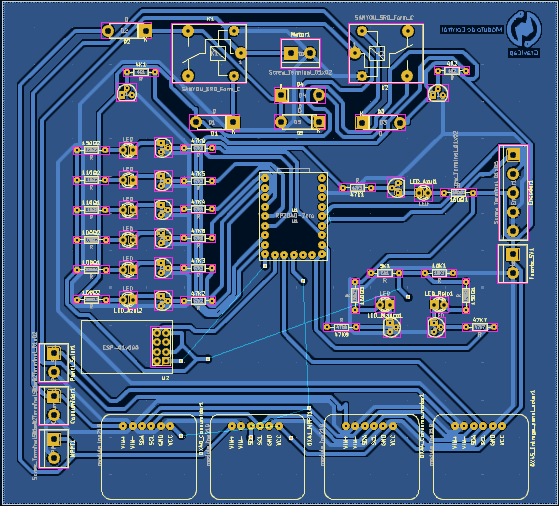
\includegraphics[width=0.8\linewidth]{Hardware/PCB.png}
                    \caption{PCB del Sistema de Control}
                    \label{fig:h1}
                \end{figure}
\chapter{Aplicación}

    \section{Función de la aplicación}
        La aplicación móvil tiene como objetivo mostrarle al usuario los distintos tipos de valores de la batería en tiempo real. Esto lo hará por medio de pantallas destinadas a los valores e interacciones que necesite el usuario, contando con gráficos interactivos. Los datos mostrados en la aplicación son subidos desde una base de datos. Contando también con una sección para contactarnos, por medio de nuestras redes sociales y página web.\par
        Con esta aplicación, el usuario podrá saber, en todo momento, los valores que necesite de la batería, como por ejemplo, la entrega que tiene la batería hacia el dispositivo que esté alimentando o, para un perfil más técnico, valores del panel solar y gráficos para más detalles sobre la misma.\par

    \section{Desarrollo del mockup de la aplicación}
    
        \subsection{Mockup}
            	Para poder desarrollar la aplicación, se necesita tener un Mockup. Su función es proveer al desarrollador el prototipo de funcionamiento, planteado de forma ilustrativa, el cual, da un primer vistazo estético, funcional e informativo de cómo será la misma. \par
                Esto conlleva plantear el diseño, e información que contendrá la aplicación , para que, posteriormente, el desarrollo final de la aplicación, se base en el Mockup, siendo de esta forma, más cómodo y práctico poder desarrollarla.\par
                La página que se designó para realizar el Mockup, fue “\href{https://marvelapp.com}{Marvel}”.\par
                Dentro de este, pueden haber varios cambios según vaya avanzando y se necesite, ya que, al fin y al cabo, es a modo ilustrativo para después poder desarrollar la aplicación final.\par
                
                \begin{figure}[H]
                    \centering
                    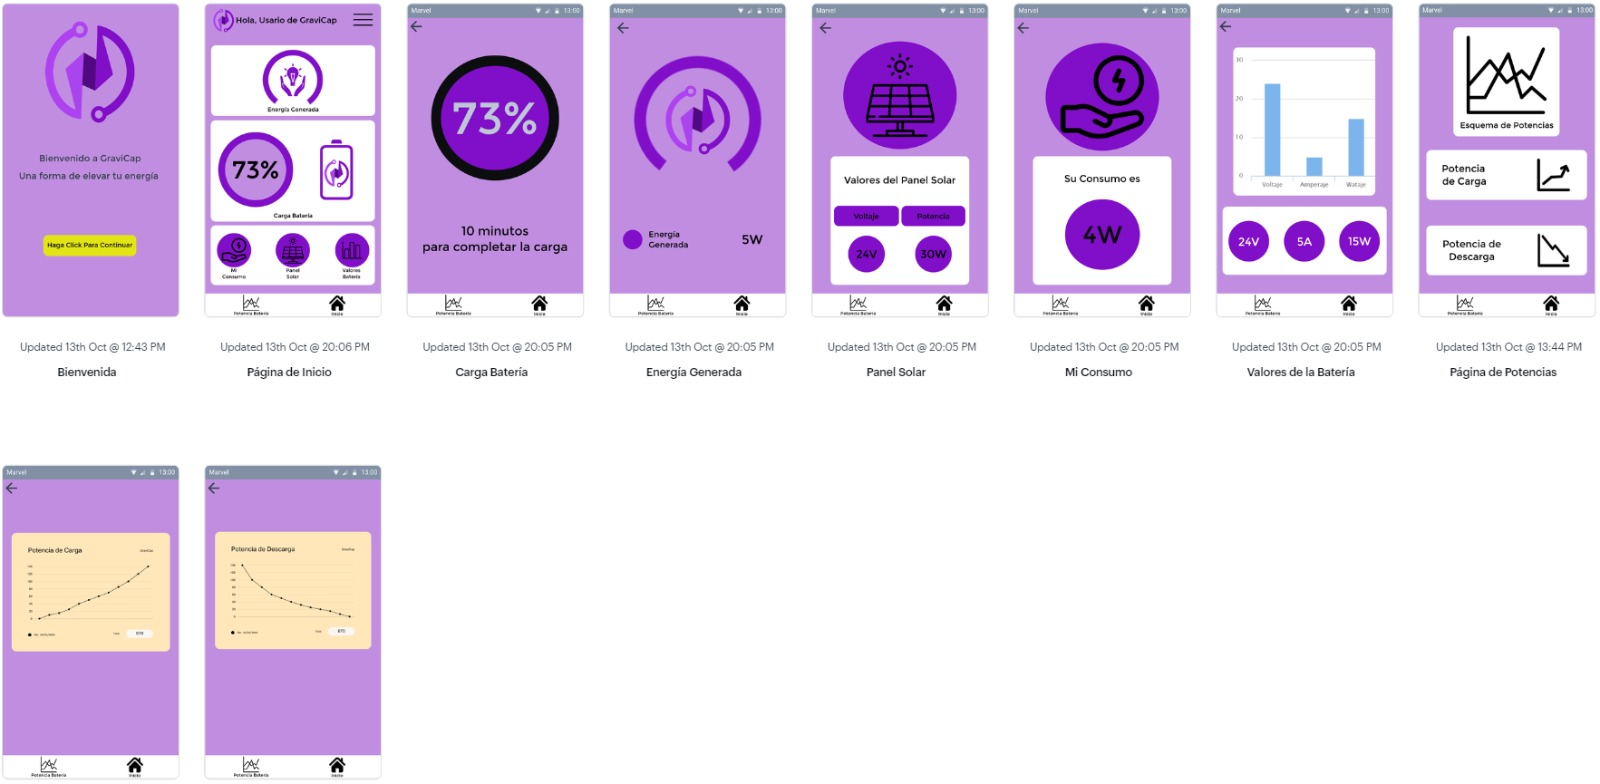
\includegraphics[width=0.8\linewidth]{Aplicación/Mockup.png}
                    \caption{Mockup de la aplicación.}
                    \label{fig:a14}
                \end{figure}
                
            \subsection{UI/UX}
                La \textbf{UX} (Experiencia de Usuario) es la experiencia integral y el conjunto de interacciones que tienen los usuarios con la misma.\par
                En cuanto a la \textbf{UI} (Interfaz de Usuario) consiste en toda la arquitectura de información, patrones y diferentes elementos visuales que nos permitan explorar la funcionalidad de la aplicación de forma eficaz y gratificante.\par
                Con esto, el usuario podrá tener una interacción “amigable” con la aplicación, siendo más cómodo y práctico moverse dentro de la misma para ver lo que necesite.\par
                La diferencia entre estos, es que la UX se centra en la manera en que el usuario interactúa con el producto de manera eficaz y, por otro lado, la UI busca ofrecer una experiencia estética satisfactoria.\par

            \subsection{User Journey}
                Para el desarrollo de la aplicación se planteó utilizar como metodología, una “jornada de usuario”. Esta metodología, plantea un mapa de recorrido del usuario en nuestra aplicación, representando así, su experiencia visual e interactiva con la misma. Pudiendo así, plantear el desarrollo del Mockup enfocándonos en el proceso que realizaría nuestro usuario dentro de la aplicación y su perspectiva.\par
                El proceso para esta metodología es buscar la empatía con el usuario, comprendiendo la relación y puntos de contacto que este tiene. Analizar sus acciones y procesos, para así, determinar lo que necesita. Con esto, se puede generar una mejor experiencia para el usuario y un proceso más eficiente.\par
                Facilita tanto el desarrollo de la aplicación como el proyecto en sí, generando una experiencia del usuario y requerimientos para el mismo. También se relaciona directamente con la UI/UX y facilita un mejor y cómodo planteamiento para las mismas.\par
                Esta herramienta o metodología, nos permite generar un usuario para así comprender y mejorar su experiencia dentro de la aplicación, así también, dándonos un mejor desarrollo dentro de nuestro proyecto.\par

                
        \section{Estructura de la Aplicación}
        
            \subsection{Editor de Código y Framework}
                Para el desarrollo de la aplicación, se utilizó el editor de código “Visual Studio Code”, en conjunto con “\href{https://ionicframework.com}{Ionic}" un framework de código abierto, proporcionandonos comodidad y amplias opciones de herramientas para el desarrollo, conteniendo varias opciones para la implementación en varios lenguajes.
                
            \subsection{Lenguajes Utilizados}
                Los lenguajes utilizados fueron HTML, CSS, JS y, como principal, React. Siendo este último, el lenguaje principal para el uso de las herramientas que nos provee Ionic.\par
                
        \section{Componentes}
        
            \subsection{WelcomePage.tsx}
            
                Este componente es el primero que se ve al iniciar la aplicación, su función consta de darle una pequeña bienvenida al usuario, explicando un poco sobre la batería y el proyecto, con un botón que lo envía a la pantalla de inicio una vez que el usuario quiera.\par

                \begin{figure} [H]
                    \centering
                    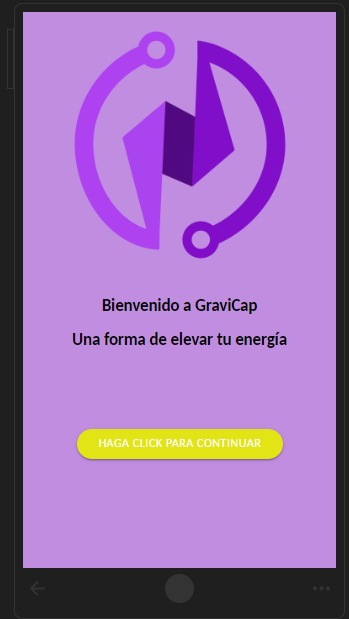
\includegraphics[width=0.25\linewidth]{Aplicación/Welcome.png}
                    \caption{Página de Bienvenida}
                    \label{fig:a1}
                \end{figure}
                
            \subsection{StartPage.tsx}
                Una vez vista la pantalla de bienvenida, el usuario es reenviado hacia la pantalla de inicio, la cual, es la pantalla principal de la aplicación, esta contiene los botones con links hacia las distintas pantallas de valores. También consta de los tabs, los cuales nos van a permitir movilizar al usuario hacia la página de los gráficos de potencia.\par
                En el apartado de arriba a la derecha encontramos un botón de información, el cual contiene los links hacia nuestro contacto y diversas redes sociales.\par

                \begin{figure} [H]
                    \centering
                    \begin{subfigure}{0.4\textwidth}
                        \centering
                        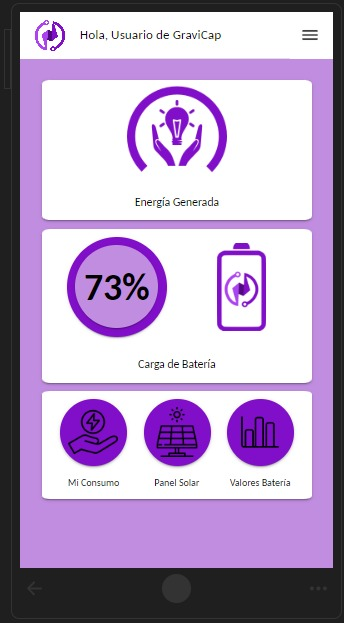
\includegraphics[width=0.7\textwidth]{Aplicación/Start.png}
                        \caption{Página de Inicio}
                        \label{fig:a2.1}
                    \end{subfigure}
                    \begin{subfigure}{0.4\textwidth}
                        \centering
                        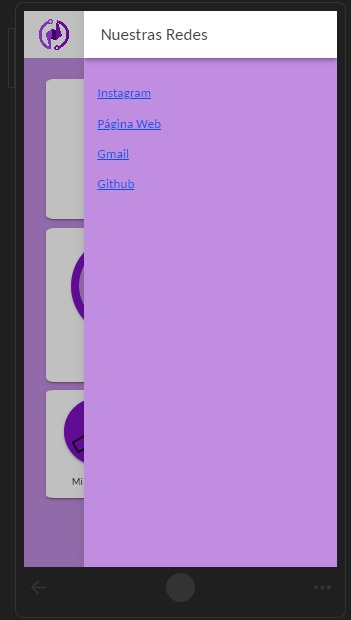
\includegraphics[width=0.7\textwidth]{Aplicación/Start_Menu.png}
                        \caption{Menú de Inicio}
                        \label{fig:a2.2}
                    \end{subfigure}
                    \hfill
                            
                    \caption{Ambas partes de la Página de Inicio}
                    \label{fig:a2}
                    \end{figure}
                
            \subsection{GeneratedEnergy.tsx}
                Este componente contiene un valor importante y recurrente para el usuario, el cual es la energía generada por la batería. Este valor le provee al usuario el valor de cuánta potencia está entregando hacia su dispositivo.\par

                \begin{figure} [H]
                    \centering
                    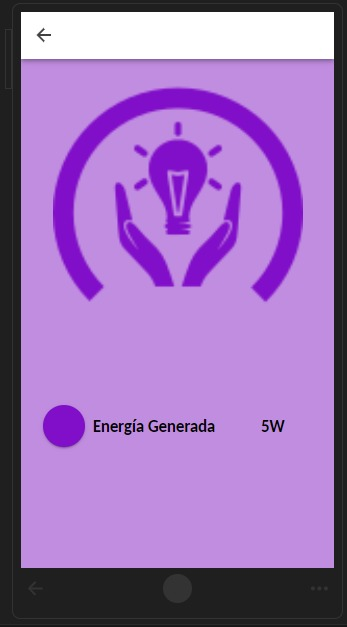
\includegraphics[width=0.25\linewidth]{Aplicación/Generated.png}
                    \caption{La cantidad de energía generada (Los valores son de referencia)}
                    \label{fig:a3}
                \end{figure}
                
            \subsection{BatteryCharge.tsx}
                Para el usuario, también es importante saber cuál es la carga de la batería, es decir, en este caso, si está en su punto más alto o más bajo. Este valor se basa en un porcentaje, el cual nos indica la posición del peso de la batería, que se traduce en un valor porcentual para el usuario. Por ejemplo, el 100\% de la batería, se da cuando el peso está en su punto más bajo, ya habiendo transformado toda la energía potencial.\par

                \begin{figure} [H]
                    \centering
                    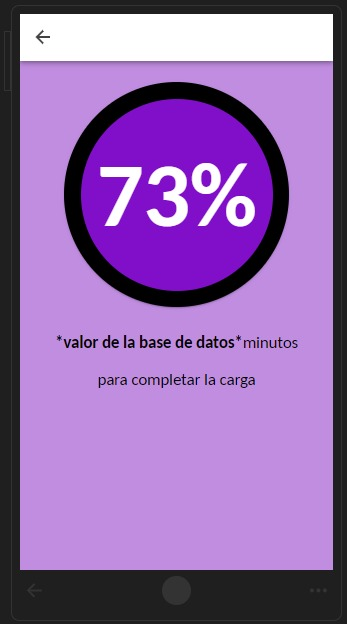
\includegraphics[width=0.25\linewidth]{Aplicación/Charge.png}
                    \caption{Carga de la batería (Los valores son de referencia)}
                    \label{fig:a4}
                \end{figure}
                
            \subsection{MyConsumption.tsx}
                El usuario también necesita saber el consumo de su dispositivo. Ese es el funcionamiento de este componente. Dándole el valor en unidad de potencia.\par

                \begin{figure} [H]
                    \centering
                    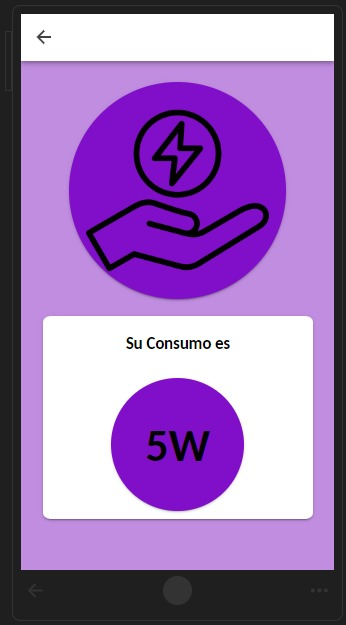
\includegraphics[width=0.25\linewidth]{Aplicación/Consumption.png}
                    \caption{El consumo del usuario (Los valores son de referencia)}
                    \label{fig:a5}
                \end{figure}
                
            \subsection{SolarPanel.tsx}
                Para saber los valores de entrega del panel solar, el usuario puede verlos dentro de la pantalla del panel solar.\par
                Los valores que nos da son el voltaje que entrega y su potencia. Todo esto en tiempo real.\par

                \begin{figure} [H]
                    \centering
                    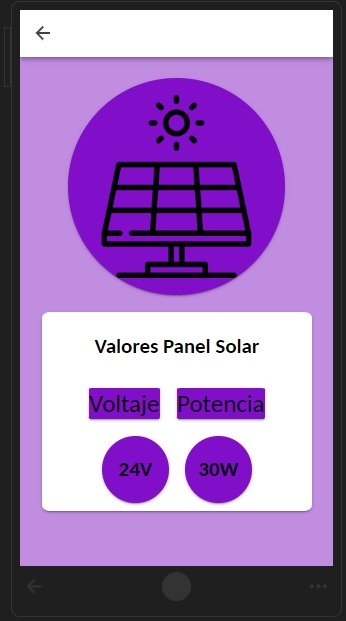
\includegraphics[width=0.25\linewidth]{Aplicación/Value_Energy.png}
                    \caption{Valor del panel solar utilizado (Los valores son de referencia)}
                    \label{fig:a6}
                \end{figure}
                
            \subsection{BatteryValues.tsx}
                Para registrar la batería y sus valores varios, en la pantalla de valores de batería el usuario podrá ver valores como Voltaje, Corriente y Potencia de la batería.\par

                \begin{figure} [H]
                    \centering
                    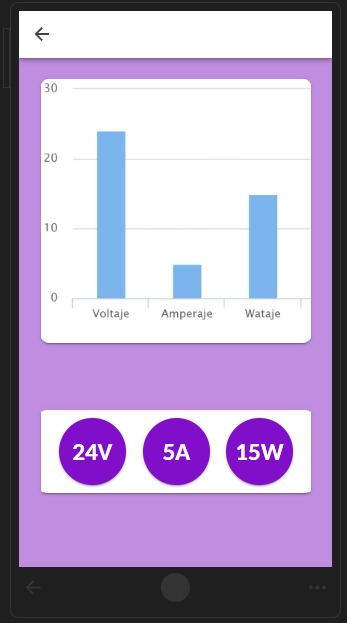
\includegraphics[width=0.25\linewidth]{Aplicación/Value_Battery.png}
                    \caption{Valor de la batería (Los valores son de referencia)}
                    \label{fig:a7}
                \end{figure}

            \subsection{GraphicsPage.tsx}
                En este apartado, el cual el usuario puede acceder desde el tab, encontraremos dos botones los cuales contienen los gráficos de carga y descarga de la batería.\par

                \begin{figure} [H]
                    \centering
                    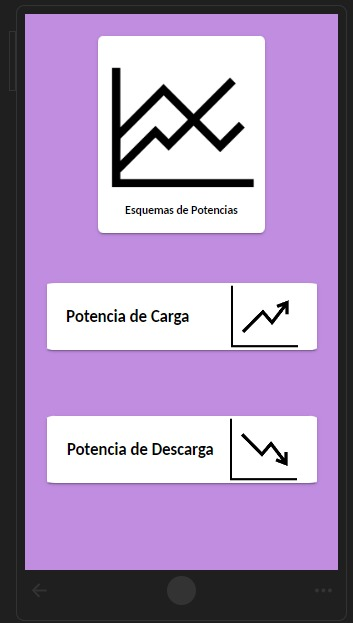
\includegraphics[width=0.25\linewidth]{Aplicación/Graphics_Page.png}
                    \caption{Página de Gráficos}
                    \label{fig:a8}
                \end{figure}

            \subsection{ChargingPowerGraphics.tsx}
                En este encontramos un gráfico de carga, el cual se basa en la potencia que entrega la batería en función del tiempo.\par
                Este funciona cuando la batería se encuentra en estado de carga, es decir, cuando está ascendiendo. Será un gráfico en ascenso.\par

                \begin{figure} [H]
                    \centering
                    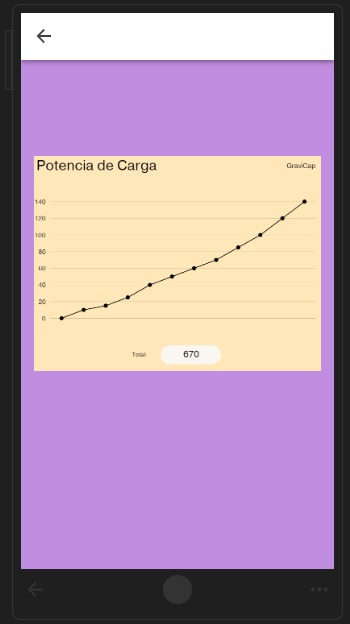
\includegraphics[width=0.25\linewidth]{Aplicación/Graphics_Charge.png}
                    \caption{Gráfico de Carga (Los valores son de referencia)}
                    \label{fig:a9}
                \end{figure}

            \subsection{DischargePowerGraphics.tsx}
                En este encontramos un gráfico de descarga, el cual se basa en la potencia que entrega la batería en función del tiempo.\par
                Este funciona cuando la batería se encuentra en estado de descarga, es decir, cuando está descendiendo. Será un gráfico en descenso.\par

                \begin{figure} [H]
                    \centering
                    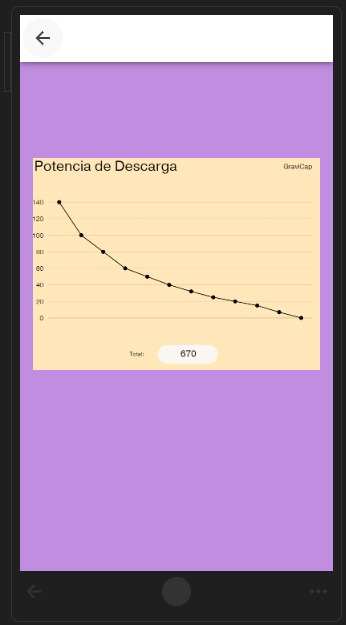
\includegraphics[width=0.25\linewidth]{Aplicación/Graphics_Discharge.png}
                    \caption{Gráfico de Descarga (Los valores son de referencia)}
                    \label{fig:a10}
                \end{figure}

            \subsection{Tabs.tsx}
                Este componente es la barra de botones que se encuentra en la parte de abajo, este contiene un botón que te redirecciona hacia la pantalla de inicio y otra que te redirecciona hacia la parte los gráficos de potencia. Dándole una mayor accesibilidad al usuario hacia las pantallas del Tab.\par

            \subsection{main.tsx}
                El main es un componente el cual no es visible, dentro de la aplicación. Este se encarga de poder ejecutar las rutas declaradas dentro del archivo App.tsx.\par

            \subsection{App.tsx}
                Este componente tampoco es visible, ya que se encarga de declarar las rutas dentro de la aplicación. Por ejemplo, puede realizar que al abrir la aplicación, redireccione al usuario hacia la pantalla de bienvenida.\par
                
        \section{Desarrollo}
            Para el desarrollo de la aplicación, se descargó \textbf{Ionic}, configurando su descarga para la utilización de herramientas y templates con el lenguaje de programación de \textbf{React}. Para poder programar y utilizar las herramientas descargadas se utilizó el editor de código de \textbf{Visual Studio Code}.\par 
            \subsection{Base de Datos}
                Teniendo como base de desarrollo el Mockup, facilita la programación de la misma. También cabe resaltar que mediante se desarrolla la aplicación en sí, el Mockup puede ir variando o la aplicación puede no ser completamente fiel estética y visualmente al mismo, quedando la aplicación final, diferente al Mockup, esto ya que se utiliza como una primera base.\par 
                Mediante el proceso se encuentran nuevas herramientas que se adapten mejor a las necesidades del momento, reescribiendo o modificando el Mockup según se requiera para una mejor versión de la aplicación.\par
            \subsection{Creación de Archivos}
                Se crearon los distintos archivos que funcionarán como componentes para la creación de las pantallas de la aplicación, desarrollando y programando así la estructura de cada uno, importando las carpetas y herramientas para cada archivo.\par

            \subsection{Herramientas de Ionic}
                Para el desarrollo de programación de los archivos se necesitó tener conocimientos dentro del lenguaje de HTML para poder programar su estructura y combinarse con el lenguaje principal React y las herramientas que provee, creando así, componentes .tsx como archivos principales para el desarrollo. En cuanto a las herramientas que nos provee Ionic, se investigó en el Framework sobre sus templates e información del uso de las herramientas más convenientes para el desarrollo de los archivos. Para poder estilizarlos según queramos, se necesitó también tener conocimientos en CSS. Para los gráficos, importados de carpetas, se necesitó tener conocimientos básicos en JavaScript.\par
                    \subsubsection{Herramientas Principales Utilizadas en Ionic}
                        Para el desarrollo de la aplicación, se utilizaron varias herramientas que nos provee Ionic, pero algunas son de características más importantes e importante resaltar, ya sea porque se utilizaron varias veces en muchos archivos, o por el peso que tienen dentro del desarrollo.\par
                        \subsubsubsection{IonApp}
                            Para la creación de los archivos, se necesita empezar con una constante o función, en la cual iremos desarrollando el código para la creación de las pantallas, así como declarar primeramente una herramienta IonApp la cual contendrá el código y los elementos de la aplicación de Ionic, solamente se declara uno en el archivo que queramos considerar como principal.\par
                        \subsubsubsection{IonContent}
                            Otro componente importante para el desarrollo es declarar un IonContent el cual actúa de contenedor principal de los componentes de la aplicación, dando así, un área única para el contenido por fuera del Header.\par
                        \subsubsubsection{IonHeader y IonMenu}
                            IonHeader componente que actúa de barra superior central, conteniendo componentes tales como iconos, botones y texto (vistos en el Header de la pantalla de Inicio). En este mismo también se declara el componente IonMenu, un botón de información lateral ubicado en la parte superior derecha de la pantalla de inicio, proporcionando los links hacia nuestras redes sociales, contacto y página web.\par
                        \subsubsubsection{IonCard}
                            Un componente muy utilizado es el de IonCard visto en gran parte en la pantalla de inicio y utilizado en otros archivos. Actuando de contenedor de otros componentes y, a su vez, dándole una mejor estética, actuando, como dice su nombre, como una carta. Modificándose en cuanto a estilos y formas con CSS, pueden actuar de contenedores circulares, también vistos en los contenedores de "Mi Consumo", "Panel Solar" y "Valores de Batería" en la pantalla de inicio. También dándole un recuadro en las páginas de gráficos, y actuando como "botones" (declarados con el componente de NavLink los cuales, al clickearlos, nos redireccionan hacia otra pantalla.\par
                        \subsubsubsection{IonNavLink y IonBackButton}
                            Con los archivos desarrollados con sus componentes y estructuras, para el movimiento del usuario por las diferentes pantallas de estas, estos necesitan un enrutamiento para la conexión entre sí. Para esto, los componentes que provee Ionic como botones (ion-button) o cartas (ion-card) se los programó con la función de IonNavLink, funciona como un enrutamiento, el cual realiza que al clickear un botón o carta nos redireccione hacia otro componente/archivo que le designemos. Con esto, el Usuario se puede movilizar dentro de la aplicación hacia donde necesite. Así también como se redirecciona hacia un componente, puede volver hacia atrás a la pantalla anterior, esto con la herramienta IonBackButton.\par
                        \subsubsubsection{IonButton}
                            Para una mejor interacción y movimiento del usuario dentro de la aplicación, se implementaron botones (ion-button). Por ejemplo, en la pantalla de Bienvenida. Otros ubicados en la parte inferior de la página de Inicio y de Gráficos la cual le permite al usuario moverse de una forma más eficiente entre las mismas. Estos cumplen la función de redireccionar al usuario hacia su determinada pantalla, dándole posibilidad de visualizar otras pantallas y obtener otro tipo de información.\par
                        \subsubsubsection{Formato SmartPhone}
                            Ionic también nos provee una herramienta para poder ver el desarrollo del archivo que estemos programando dentro de Visual Studio Code en forma de un SmartPhone. Con esta función se facilita poder programar cada componente estructural para el desarrollo final.\par
                            
                            \begin{figure}[H]
                                \centering
                                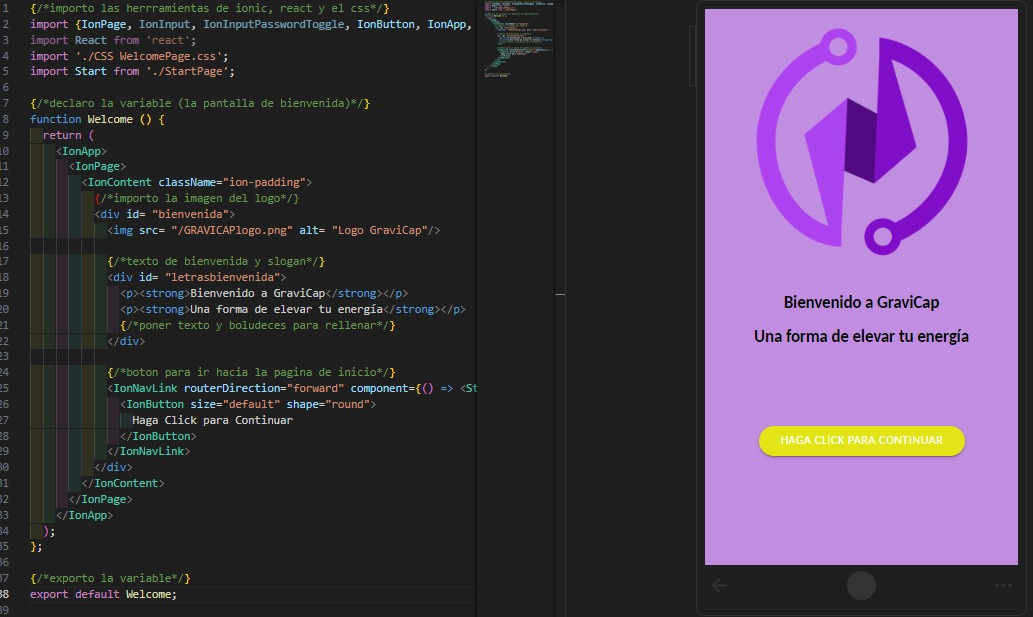
\includegraphics[width=\linewidth]{Aplicación/Code.png}
                                \caption{Imagen de Referencia de la función de Smartphone}
                                \label{fig:a15}
                            \end{figure}
                
                            Con los archivos desarrollados con sus componentes y estructuras, para el movimiento del usuario por las diferentes pantallas de estas, los componentes necesitan un enrutamiento para la conexión entre sí. Para esto, los componentes que provee Ionic como botones (\textit{ion-button}) o cartas (\textit{ion-card}) se los programó con la función de \textit{IonNavLink}, funciona como un enrutamiento, el cual realiza que al clickear un botón o carta nos redireccione hacia otro componente/archivo que le designemos. Con esto, el Usuario se puede movilizar dentro de la aplicación hacia donde necesite. Así también como se redirecciona hacia un componente, puede volver hacia atrás a la pantalla anterior, esto con la herramienta \textit{IonBackButton}.\par
                El usuario, en la pantalla de inicio, en la parte superior derecha de la misma, dispone de un botón de información, el cual, le proveerá información de nuestras redes sociales y contacto.\par
                Para un mejor movimiento del usuario dentro de la aplicación, se implementó la herramienta \textit{Tabs} (\textit{ion-tabs}). Esta es una barra ubicada en la parte inferior la cual le permite al usuario moverse de una forma más eficiente, conteniendo iconos, los cuales actúan de botones para redireccionar al usuario hacia su determinada pantalla, dándole posibilidad de visualizar otras pantallas y obtener otro tipo de información.\par
                Una vez teniendo todos los archivos programados con sus respectivas estructuras y componentes, se debe añadir estilos, darle forma a los componentes que queramos, colores y tamaños, dándoles así el vistazo estético requerido planteado en el Mockup. Para esto, cada componente necesita sus estilos, creándose así un archivo \textit{CSS} individual para cada uno. Estos se programan y se importan al archivo que se requiera, modificando su estructura y tamaños dándole un mejor acabado estético para el usuario.\par
            \subsection{Estilos y CSS}
                Una vez teniendo todos los archivos programados con sus respectivas estructuras y componentes, se debe añadir estilos, darle forma a los componentes que queramos, colores y tamaños, dándoles así el vistazo estético requerido planteado en el Mockup. Para esto, cada componente necesita sus estilos, creándose así un archivo CSS individual para cada uno. Estos se programan y se importan al archivo que se requiera, modificando su estructura y tamaños dándole un mejor acabado estético para el usuario.\par
            \subsection{Gráficos}
            \subsection{Servidor}
\chapter{Página Web}
    
    \section{Introducción}
    
        La página web desarrollada para \textcolor{dark_violet}{\textbf{GraviCap}} juega un papel fundamental en la difusión y comunicación del proyecto. Su creación responde a la necesidad de tener una plataforma en línea donde se pueda acceder fácilmente a toda la información relevante sobre el proyecto, sus objetivos, sus integrantes y las fases de desarrollo. Este sitio web no solo sirve como un medio de promoción, sino que también actúa como un canal interactivo entre el equipo y el público interesado.\par
        A lo largo del desarrollo del proyecto, consideramos esencial contar con una herramienta que fuera accesible para cualquier persona interesada en conocer más sobre \textcolor{dark_violet}{\textbf{GraviCap}}. Por ello, el sitio web se construyó con un diseño intuitivo y funcional, con el objetivo de proporcionar información clara y precisa, así como facilitar la interacción directa con los visitantes a través de un formulario de contacto. Asimismo, la página está pensada para ser compatible con dispositivos móviles y de escritorio, asegurando que cualquier usuario pueda acceder a la información sin inconvenientes, independientemente del dispositivo que utilice.\par
        Este capítulo describe en detalle el propósito de la página web, su estructura técnica, los componentes que la componen y el proceso seguido para su implementación. Desde la creación de los componentes en Vue.js hasta su despliegue final utilizando Vercel.app, se documentan los pasos clave y las decisiones técnicas que permitieron la construcción de un sitio web eficiente y profesional para el proyecto \textcolor{dark_violet}{\textbf{GraviCap}}.\par

    \section{Función}
        El objetivo principal de la página web es proporcionar una plataforma accesible para que los usuarios interesados en el proyecto \textcolor{dark_violet}{\textbf{GraviCap}} puedan obtener más información sobre el mismo, conocer a los integrantes del equipo y entender el proceso que llevó al desarrollo del proyecto desde su concepción hasta la implementación final. Además, la página web ofrece la posibilidad de que los usuarios se pongan en contacto con nosotros a través de un formulario de contacto, facilitando la comunicación directa por correo electrónico. La promoción de la página se realizará mediante un enlace compartido en la cuenta de Instagram de \textcolor{dark_violet}{\textbf{GraviCap}}, usando una herramienta de linktree, lo que asegurará su visibilidad en las redes sociales.\par
        
    \section{Estructura}
            \subsection{Componentes}
                La estructura de la página web está organizada de manera modular, dividiéndose en varios componentes que permiten la navegación sencilla entre las diferentes secciones. Estos componentes fueron desarrollados en Vue.js, lo que facilita su integración y reutilización en diferentes partes de la página. Se crearon cuatro componentes principales, cada uno con una funcionalidad específica, y un componente adicional que es común en todas las rutas de la página.\par
                
                \subsubsection{App.vue}
                    El componente App.vue se mantiene activo sin importar la ruta seleccionada dentro de la página web, sirviendo como una estructura común a todas las secciones. Este componente contiene un header con el logotipo de \textcolor{dark_violet}{GraviCap} y un texto con el nombre del proyecto, ambos actuando como enlaces que redirigen al subcomponente Home. Además, se incluyen tres opciones de navegación: Sobre Nosotros, Galería y Contáctanos, que funcionan como rutas hacia sus respectivos subcomponentes. También se han añadido iconos para redirigir a las cuentas de Instagram y GitHub del proyecto, facilitando el acceso directo a las redes sociales y al repositorio del código.\par
                    
                    \begin{figure}[!ht]
                        \centering
                        
\includegraphics[width=\linewidth]{Página Web/App.png}
                        \caption{Componente de App.vue}
                        \label{fig:pw1}
                    \end{figure}
                    
                \subsubsection{HomeView.vue}
                    El subcomponente HomeView.vue es la página principal que se carga por defecto al ingresar al sitio. Está dividida en dos partes: un grid a la izquierda que contiene el eslogan del proyecto junto con un resumen breve y claro sobre el propósito de \textcolor{dark_violet}{GraviCap}, y un grid a la derecha que presenta un título con tres subtítulos explicando los beneficios clave del proyecto. Este subcomponente proporciona al usuario una visión general inmediata de lo que trata el proyecto y sus ventajas.\par
                    
                    \begin{figure} [H]
                    \centering
                    \begin{subfigure}{0.5\textwidth}
                        \centering
                        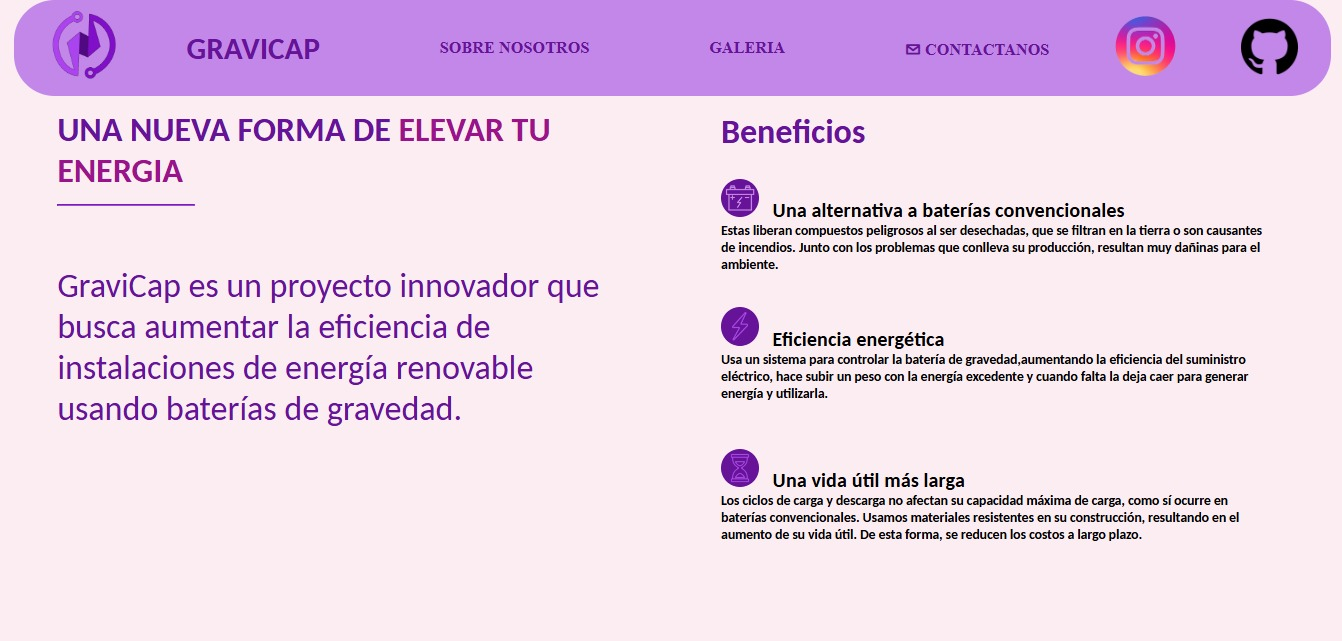
\includegraphics[width=\textwidth]{Página Web/Computadora/HomeScreen.png}
                        \caption{Computadora}
                        \label{fig:pw2.1}
                    \end{subfigure}
                    \hfill
                    \begin{subfigure}{0.4\textwidth}
                        \centering
                        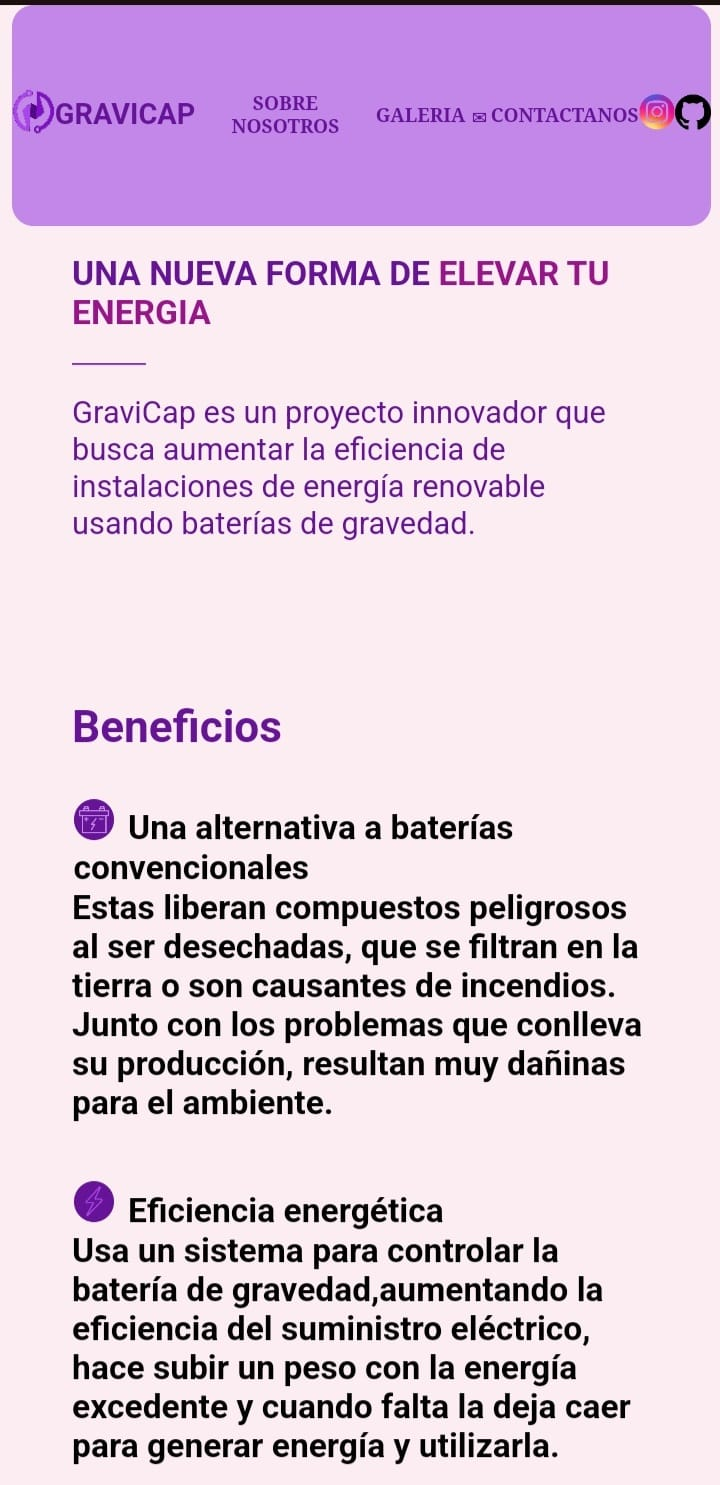
\includegraphics[width=0.5\textwidth]{Página Web/Celular/Homescreen.png}
                        \caption{Celular}
                        \label{fig:pw2.2}
                    \end{subfigure}
                    \hfill
                            
                    \caption{Componente de HomeView.vue}
                    \label{fig:pw2}
                    \end{figure}
                    
                \subsubsection{NosotrosView.vue}
                    Este subcomponente, NosotrosView.vue, está organizado en dos secciones principales. A la izquierda, el título "¿Quiénes Somos?" ofrece una explicación sobre el origen del equipo de trabajo, los objetivos del grupo y el propósito detrás de este proyecto. A la derecha, se muestra una galería de imágenes con las fotos de los integrantes del equipo, acompañadas por sus respectivos roles dentro del desarrollo del proyecto, brindando una presentación visual y detallada de quienes están detrás de \textcolor{dark_violet}{GraviCap}.\par

                    \begin{figure} [H]
                    \centering
                    \begin{subfigure}{0.5\textwidth}
                        \centering
                        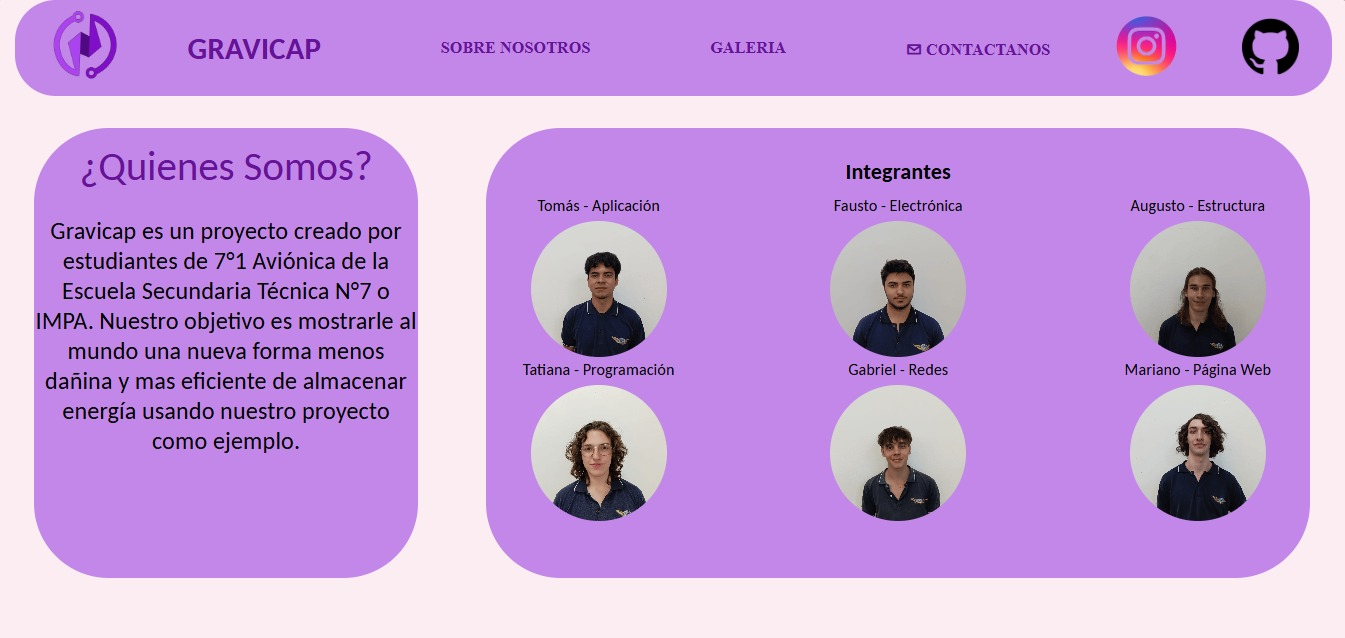
\includegraphics[width=\textwidth]{Página Web/Computadora/Integrantes.png}
                        \caption{Computadora}
                        \label{fig:pw3.1}
                    \end{subfigure}
                    \hfill
                    \begin{subfigure}{0.4\textwidth}
                        \centering
                        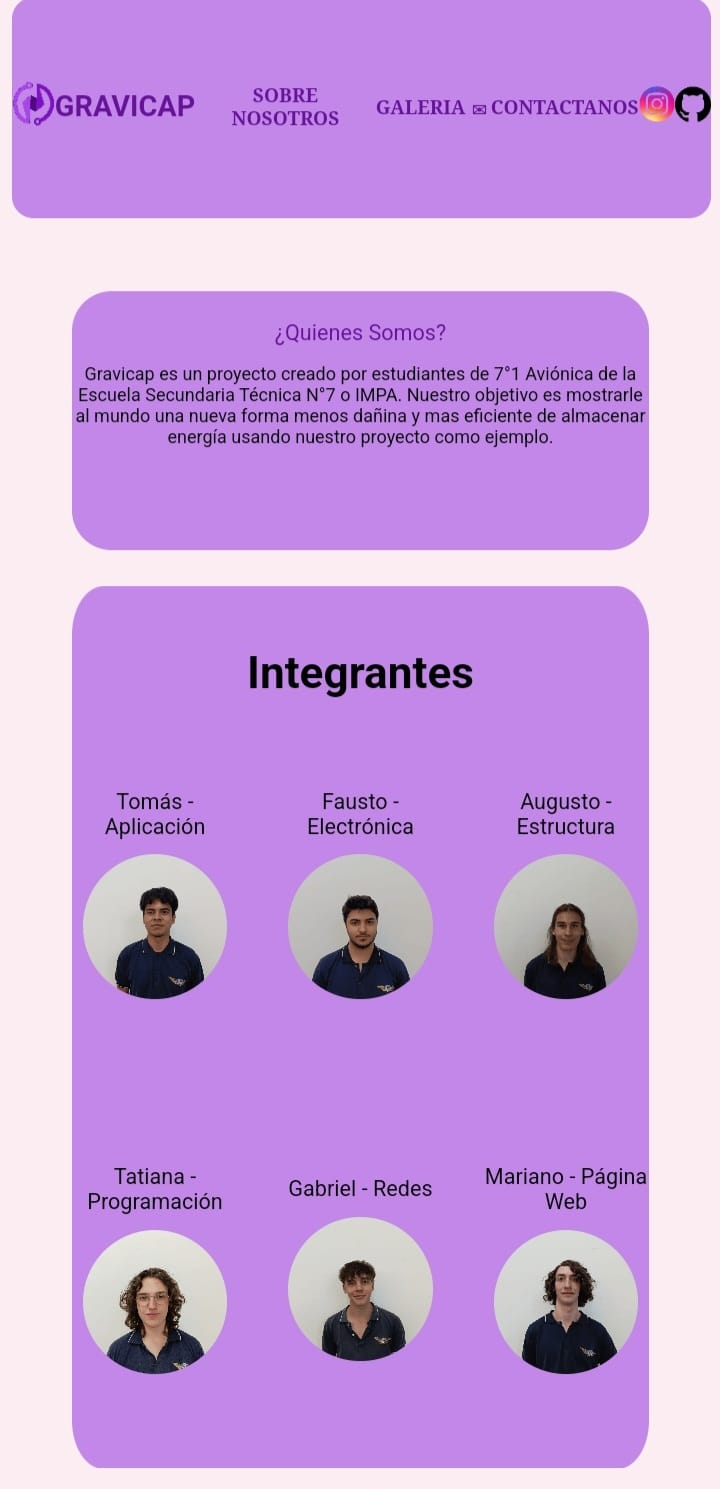
\includegraphics[width=0.5\textwidth]{Página Web/Celular/Integrantes.png}
                        \caption{Celular}
                        \label{fig:pw3.2}
                    \end{subfigure}
                    \hfill
                            
                    \caption{NosotrosView.vue}
                    \label{fig:pw3}
                    \end{figure}
                    
                \subsubsection{GaleríaView.vue}
                    El subcomponente GaleríaView.vue se encarga de mostrar las imágenes más relevantes relacionadas con el proyecto. Se organiza en un diseño de grid con múltiples columnas, donde cada imagen está acompañada de un título que explica brevemente de qué trata. Este subcomponente permite a los usuarios explorar visualmente el desarrollo y avances del proyecto a lo largo del tiempo.\par

                    \begin{figure} [H]
                    \centering
                    \begin{subfigure}{0.5\textwidth}
                        \centering
                        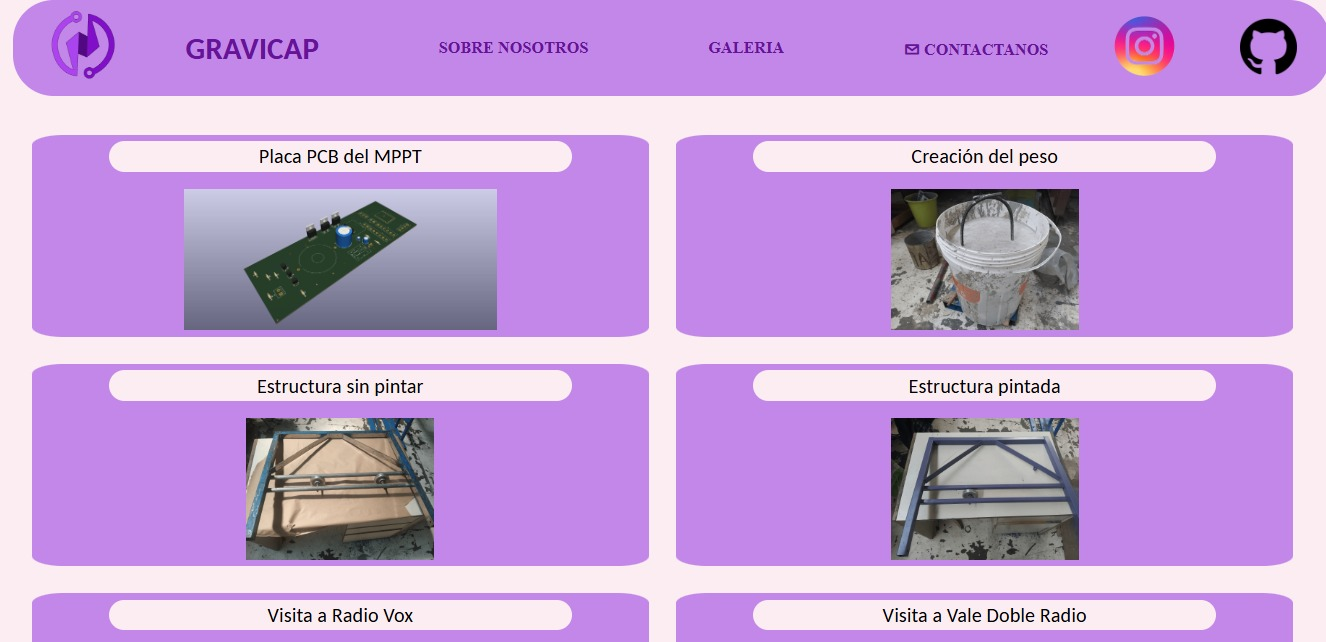
\includegraphics[width=\textwidth]{Página Web/Computadora/Galería.png}
                        \caption{Computadora}
                        \label{fig:pw4.1}
                    \end{subfigure}
                    \hfill
                    \begin{subfigure}{0.4\textwidth}
                        \centering
                        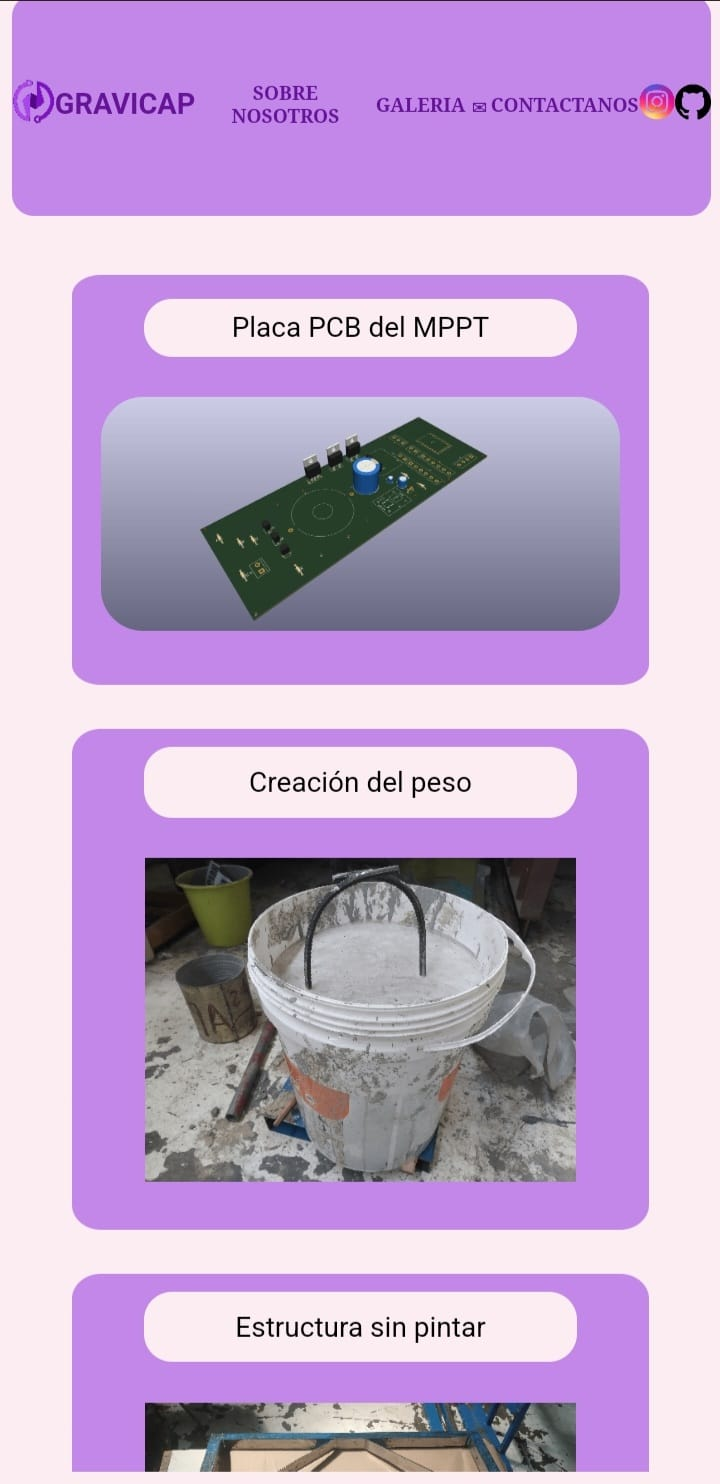
\includegraphics[width=0.5\textwidth]{Página Web/Celular/Galería.png}
                        \caption{Celular}
                        \label{fig:pw4.2}
                    \end{subfigure}
                    \hfill
                            
                    \caption{Componente de GaleríaView.vue}
                    \label{fig:pw4}
                    \end{figure}

                \subsubsection{ContactanosView.vue}
                    El subcomponente ContactanosView.vue incluye un formulario que permite a los usuarios enviarnos un mensaje directo a nuestra cuenta de Gmail del proyecto. El formulario solicita que el usuario ingrese su nombre, su correo electrónico y el mensaje que desea enviar. Una vez completado, se utiliza web3forms para procesar y enviar el mensaje, facilitando la comunicación directa entre los interesados y el equipo de \textcolor{dark_violet}{GraviCap}.\par

                    \begin{figure} [H]
                    \centering
                    \begin{subfigure}{0.5\textwidth}
                        \centering
                        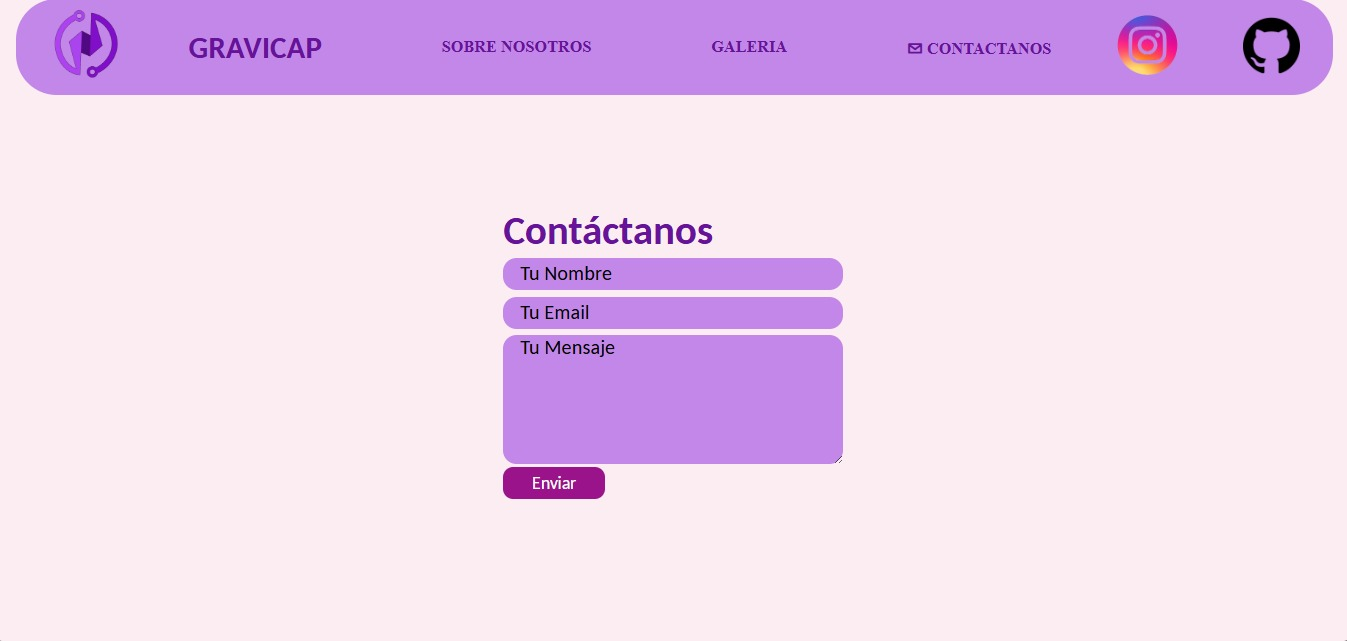
\includegraphics[width=\textwidth]{Página Web/Computadora/Contactos.png}
                        \caption{Computadora}
                        \label{fig:pw5.1}
                    \end{subfigure}
                    \begin{subfigure}{0.4\textwidth}
                        \centering
                        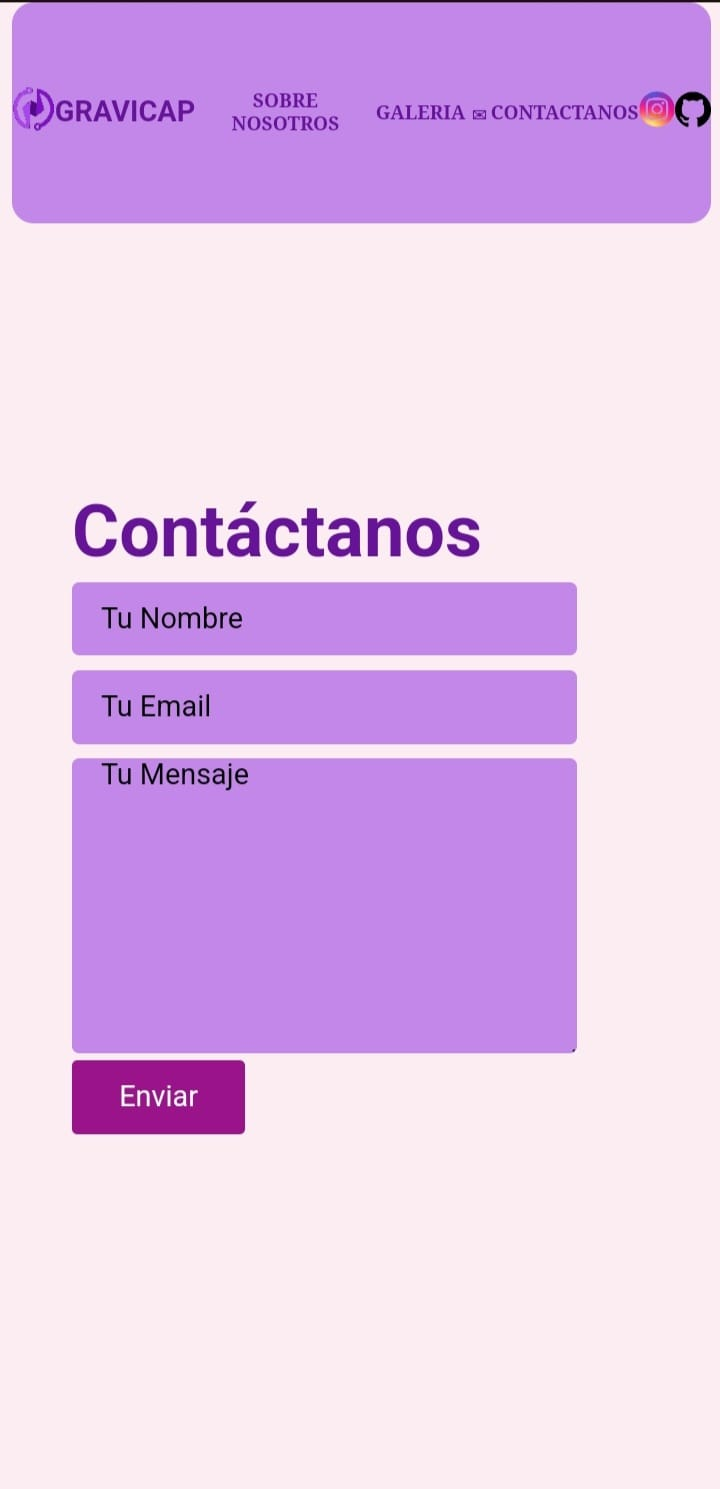
\includegraphics[width=0.5\textwidth]{Página Web/Celular/Contactos.png}
                        \caption{Celular}
                        \label{fig:pw5.2}
                    \end{subfigure}
                    \hfill
                            
                    \caption{Componente de ContactanosView.vue}
                    \label{fig:pw5}
                    \end{figure}
                    
    \section{Proceso}
        El desarrollo de la página web comenzó con la creación de los componentes principales en archivos separados de HTML y CSS, que definían tanto la estructura visual como la funcionalidad básica de cada parte de la página. El HTML se utilizó para definir la base de cada componente, mientras que el CSS permitió estilizar estos elementos y asegurarse de que fueran responsivos, es decir, que se ajustaran correctamente a diferentes tamaños de pantalla.\par
        Una vez diseñados estos componentes, se convirtieron en archivos .vue que incluyen tanto los estilos en CSS dentro de un bloque \texttt{<style scoped>} como la estructura HTML en un bloque \texttt{<template>}, permitiendo la integración en el framework Vue.js. Los componentes principales (HomeView.vue, ContactanosView.vue, GaleríaView.vue y NosotrosView.vue) fueron organizados en la carpeta views, mientras que el archivo App.vue se configuró para contener el header y permitir la navegación entre las distintas secciones de la página.\par
        Finalmente, se creó un archivo index.js para manejar las rutas entre los diferentes componentes, facilitando la navegación entre las distintas secciones del sitio. El proyecto fue desplegado utilizando Vercel.app, una plataforma que permite alojar proyectos web fácilmente, y está disponible en el repositorio de GitHub del proyecto.\par
\chapter{Limitaciones y Próximos Pasos}

    \section{Limitaciones}
        Durante el desarrollo del proyecto \textcolor{dark_violet}{GraviCap}, nos enfrentamos a varias limitaciones propias de trabajar con recursos restringidos y bajo las condiciones de un grupo de estudiantes en una escuela secundaria técnica. Estas limitaciones afectaron tanto el diseño como la implementación del prototipo, pero también nos ofrecieron valiosas lecciones sobre cómo escalar y mejorar el sistema en el futuro.\par
        
        \subsection{Capacidad de Almacenamiento de Energía}
        
            Una de las principales limitaciones del prototipo es la capacidad de almacenamiento de energía, que está determinada principalmente por la masa utilizada y la altura a la que puede ser elevada. El sistema actual utiliza una masa de 27 kg y una altura de 2,2 metros, lo que permite almacenar una cantidad limitada de energía potencial gravitatoria. Aunque esto es suficiente para demostrar el principio de funcionamiento del sistema, resulta insuficiente para aplicaciones a gran escala. La fórmula de la energía potencial, $E_p = mgh$, muestra que, para aumentar la capacidad de almacenamiento, sería necesario elevar la masa a mayores alturas o utilizar cargas más pesadas, lo que presenta desafíos adicionales en términos de infraestructura y control.\par
            
        \subsection{Eficiencia del Motor/Generador}
        
            Otro desafío importante fue la eficiencia del motor/generador. El prototipo utiliza un motor con una potencia de 195W y una reducción significativa de la velocidad, de 8100 RPM a 11 RPM. Aunque este sistema ha demostrado ser funcional para el prototipo, las pérdidas de energía durante la conversión de energía potencial en energía eléctrica siguen siendo un problema. Los motores utilizados para la generación de energía en aplicaciones industriales suelen tener una mayor eficiencia, lo que sugiere que, para futuras versiones del proyecto, sería necesario invertir en motores de mejor calidad y reducir las fricciones mecánicas en el sistema.\par
            
        \subsection{Infraestructura Limitada}
            El espacio disponible y los materiales utilizados también representaron una limitación. Nuestro prototipo fue diseñado y construido con materiales reciclados y reutilizados, lo cual tiene un impacto positivo en el costo y la sostenibilidad del proyecto. Sin embargo, para un sistema comercialmente viable, la infraestructura debe ser más robusta y estar diseñada específicamente para soportar grandes cargas durante largos períodos de tiempo sin riesgo de deterioro estructural.\par
    
    \section{Próximos Pasos}
    
        A pesar de las limitaciones mencionadas, el proyecto \textcolor{dark_violet}{GraviCap} tiene un enorme potencial para ser escalado y mejorado, no solo a nivel técnico, sino también en cuanto a su impacto en el almacenamiento de energía renovable. Basándonos en lo aprendido durante el desarrollo del prototipo, los próximos pasos a seguir incluirán tanto mejoras en el diseño del sistema como la implementación de nuevas tecnologías para aumentar su eficiencia y capacidad.\par
        
        \subsection{Escalado del Sistema}
        
            El paso más inmediato es aumentar la escala del sistema. Esto implicará la construcción de una versión más grande del prototipo, utilizando masas más pesadas y elevándolas a mayores alturas para incrementar la capacidad de almacenamiento de energía. Además, se considerarán nuevas configuraciones que permitan optimizar el uso del espacio y mejorar la conversión de energía potencial en electricidad.\par
            
        \subsection{Optimización del Motor/Generador}
        
            Se buscarán motores y generadores más eficientes para maximizar la cantidad de energía que se puede recuperar durante el proceso de descarga. Esto podría incluir la implementación de motores de última generación, con menores pérdidas por fricción y una mayor capacidad de conversión de energía mecánica en eléctrica. También se evaluarán nuevas configuraciones de poleas y sistemas de transmisión para reducir las pérdidas mecánicas en el sistema.\par
        
        \subsection{Ampliación de Aplicaciones}
        
            Un aspecto clave del futuro de \textcolor{dark_violet}{GraviCap} será su adaptabilidad a diferentes escenarios de uso. Aunque el prototipo actual ha sido desarrollado principalmente como una demostración a pequeña escala, el sistema podría adaptarse a necesidades específicas, como el almacenamiento de energía en zonas rurales sin acceso a la red eléctrica o como respaldo energético para sistemas solares. A medida que el proyecto crezca, se buscará que la tecnología sea accesible y económicamente viable para su implementación a distintas escalas.\par
        
        \subsection{Pruebas y Validación}
            Finalmente, es esencial que el sistema sea sometido a pruebas rigurosas en condiciones reales. Se planifican pruebas adicionales para evaluar el rendimiento del sistema en diferentes entornos, considerando factores como la temperatura, la humedad y las condiciones de carga variables. Estas pruebas ayudarán a identificar cualquier posible fallo y permitirán ajustar el diseño antes de implementar el sistema a mayor escala.\par
\chapter{Bibliografía utilizada}
    
        \section{Cargador MPPT}
        
            \begin{itemize} [label=•]
                \setlength{\itemindent}{3em}
                \item Guía en la programación (\href{https://electronoobs.com/eng_arduino_tut133.php}{https://electronoobs.com/eng\_arduino\_tut133.php})
            \end{itemize}
            
        \section{Hardware}
        
            \begin{itemize} [label=•]
                \setlength{\itemindent}{3em}
                \item a
            \end{itemize}
            
        \section{Software}
        
            \begin{itemize} [label=•]
                \setlength{\itemindent}{3em}
                \item a
            \end{itemize}
            
        \section{Página Web}
        
            \begin{itemize} [label=•]
                \setlength{\itemindent}{3em}
                \item FreeCodeCamp (Sitio Web: \href{https://www.freecodecamp.org/}{https://www.freecodecamp.org/})
                \item W3Schools Online Web Tutorials (Sitio Web: \href{https://www.w3schools.com/}{https://www.w3schools.com/})
                \item Stack Overflow (Sitio Web: \href{https://stackoverflow.com/}{https://stackoverflow.com/})
                \item How To Create Working Contact Form Using HTLM \& CSS Recieve Contact From Data on Email (Enlace: \href{https://youtu.be/-HeadgoqJ7A}{https://youtu.be/-HeadgoqJ7A})
            \end{itemize}
            
        \section{Aplicación}
        
            \begin{itemize} [label=•]
                \setlength{\itemindent}{3em}
                \item MarvelApp (Sitio Web: \href{https://marvelapp.com/}{https://marvelapp.com/})
                \item Ionic (Sitio Web: \href{https://ionicframework.com/}{https://ionicframework.com/})
                \item FreeCodeCamp (Sitio Web: \href{https://www.freecodecamp.org/}{https://www.freecodecamp.org/})
            \end{itemize}
            
        \section{Documentación}
            \begin{itemize} [label=•]
                \setlength{\itemindent}{3em}
                \item CTAN (Sitio Web: \href{https://ctan.org}{https://ctan.org})
                \item geometry (\href{https://ctan.org/pkg/geometry}{https://ctan.org/pkg/geometry})
                \item hyperref (\href{https://ctan.org/pkg/hyperref}{https://ctan.org/pkg/hyperref})
                \item babel (\href{https://ctan.org/pkg/babel}{https://ctan.org/pkg/babel})
                \item tocloft (\href{https://ctan.org/pkg/hyperref}{https://ctan.org/pkg/tocloft})
                \item carlito (\href{https://ctan.org/pkg/carlito}{https://ctan.org/pkg/carlito})
                \item inputenc (\href{https://ctan.org/pkg/inputenc}{https://ctan.org/pkg/inputenc})
                \item setspace (\href{https://ctan.org/pkg/setspace}{https://ctan.org/pkg/setspace})
                \item enumitem (\href{https://ctan.org/pkg/enumitem}{https://ctan.org/pkg/enumitem})
                \item ragged2e (\href{https://ctan.org/pkg/ragged2e}{https://ctan.org/pkg/ragged2e})
                \item titlesec (\href{https://ctan.org/pkg/titlesec}{https://ctan.org/pkg/titlesec})
                \item fancyhdr (\href{https://ctan.org/pkg/fancyhdr}{https://ctan.org/pkg/fancyhdr})
                \item xcolor (\href{https://ctan.org/pkg/xcolor}{https://ctan.org/pkg/xcolor})
                \item appendix (\href{https://ctan.org/pkg/appendix}{https://ctan.org/pkg/appendix})
                \item graphicx (\href{https://ctan.org/pkg/graphicx}{https://ctan.org/pkg/graphicx})
                \item rotating (\href{https://ctan.org/pkg/rotating}{https://ctan.org/pkg/rotating})
                \item adjustbox (\href{https://ctan.org/pkg/adjustbox}{https://ctan.org/pkg/adjustbox})
                \item pdflcape (\href{https://ctan.org/pkg/pdflscape}{https://ctan.org/pkg/pdflscape})
                \item subcaption (\href{https://ctan.org/pkg/subcaption}{https://ctan.org/pkg/subcaption})
                \item float (\href{https://ctan.org/pkg/float}{https://ctan.org/pkg/float})
                \item array (\href{https://ctan.org/pkg/array}{https://ctan.org/pkg/array})
                \item tabularx (\href{https://ctan.org/pkg/tabularx}{https://ctan.org/pkg/tabularx})
                \item tabularray (\href{https://ctan.org/pkg/tabularray}{https://ctan.org/pkg/tabularray})
                \item cancel (\href{https://ctan.org/pkg/cancel}{https://ctan.org/pkg/cancel})
                \item listings (\href{https://ctan.org/pkg/listings}{https://ctan.org/pkg/listings})
                \item Tex Stack Exchange (Sitio Web: \href{https://tex.stackexchange.com}{https://tex.stackexchange.com})
                \item Overleaf (Sitio Web: \href{https://www.overleaf.com/}{https://www.overleaf.com/})
            \end{itemize}
        \section{Investigación}
            \begin{itemize} [label=•]
                \setlength{\itemindent}{3em}
                \item Cynthia Santos Gómez. \guillemotleft Almacenamiento de Energía Potencial Gravitatoria mediante el desplazamiento de bloques sólidos por ferrocarril. Proyecto ARES.\guillemotright. En: Universidad de Sevilla (2017).
                \item Santiago Blas Marreros, Abelardo Cajaleón Alcántara, Micaela Cajaleón Alcántara, Peruska Pareja Madera, José Sánchez León Velarde, Abel Yucra Palacios, Alberto Huiman Cruz. \guillemotleft Situación de manejo de las baterías de plomo ácido en el Perú\guillemotright. En: Revista del Instituto de investigación de la Facultad de minas, metalurgia y ciencias geográficas de la Universidad Nacional Mayor de San Marcos (2022).
                \item Ing. Godelia Canchari Silverio, Ing. Oswaldo Ortiz Sanchez.\guillemotleft SISTEMA DE GESTIÓN DE RESIDUOS PELIGROSOS (PILAS Y BATERIAS) EN LA FACULTAD DE INGENIERIA GEOLOGICA, MINERA, METALURGICA Y GEOGRAFICA DE LA UNIVERSIDAD NACIONAL MAYOR DE SAN MARCOS \guillemotright. En: Revista del Instituto de investigación de la Facultad de minas, metalurgia y ciencias geográficas Volumen 13 (2010).
            \end{itemize}

\begin{appendix}

\chapter{Apéndice A: Esquemáticos}
\renewcommand{\thepage}{A-\arabic{page}}
\setcounter{page}{1}
    Este apéndice presenta los esquemáticos eléctricos desarrollados para el proyecto \textcolor{dark_violet}{\textbf{GraviCap}}. Los esquemáticos incluidos proporcionan una visión detallada de los circuitos clave que permiten el funcionamiento eficiente del sistema. Estos esquemáticos son fundamentales para comprender la implementación de los sistemas de control y gestión de energía, y sirven como guía técnica para la construcción y funcionamiento del prototipo.
    Los dos esquemáticos que se incluyen en este apéndice son:\par
    
    \begin{itemize} [label = ]
    \setlength{\itemindent}{2em}
    
        \item MPPT (Maximum Power Point Tracking): Este esquema muestra el diseño del sistema encargado de optimizar la recolección de energía desde los paneles solares, asegurando que el sistema opere en el punto de máxima eficiencia, maximizando la energía capturada y transferida a la batería.\par
        \item Sistema de Control: Este esquema describe el hardware y la lógica de control del sistema de batería gravitatoria, incluyendo los componentes encargados de gestionar el flujo de energía entre la batería y la carga, así como los sensores que permiten un control preciso del sistema.\par
    \end{itemize}
    
    Ambos esquemáticos son esenciales para el correcto funcionamiento del sistema y proporcionan las bases técnicas para futuras expansiones o modificaciones en el diseño.\par

    \begin{landscape}
        \begin{sidewaysfigure}
            \centering
            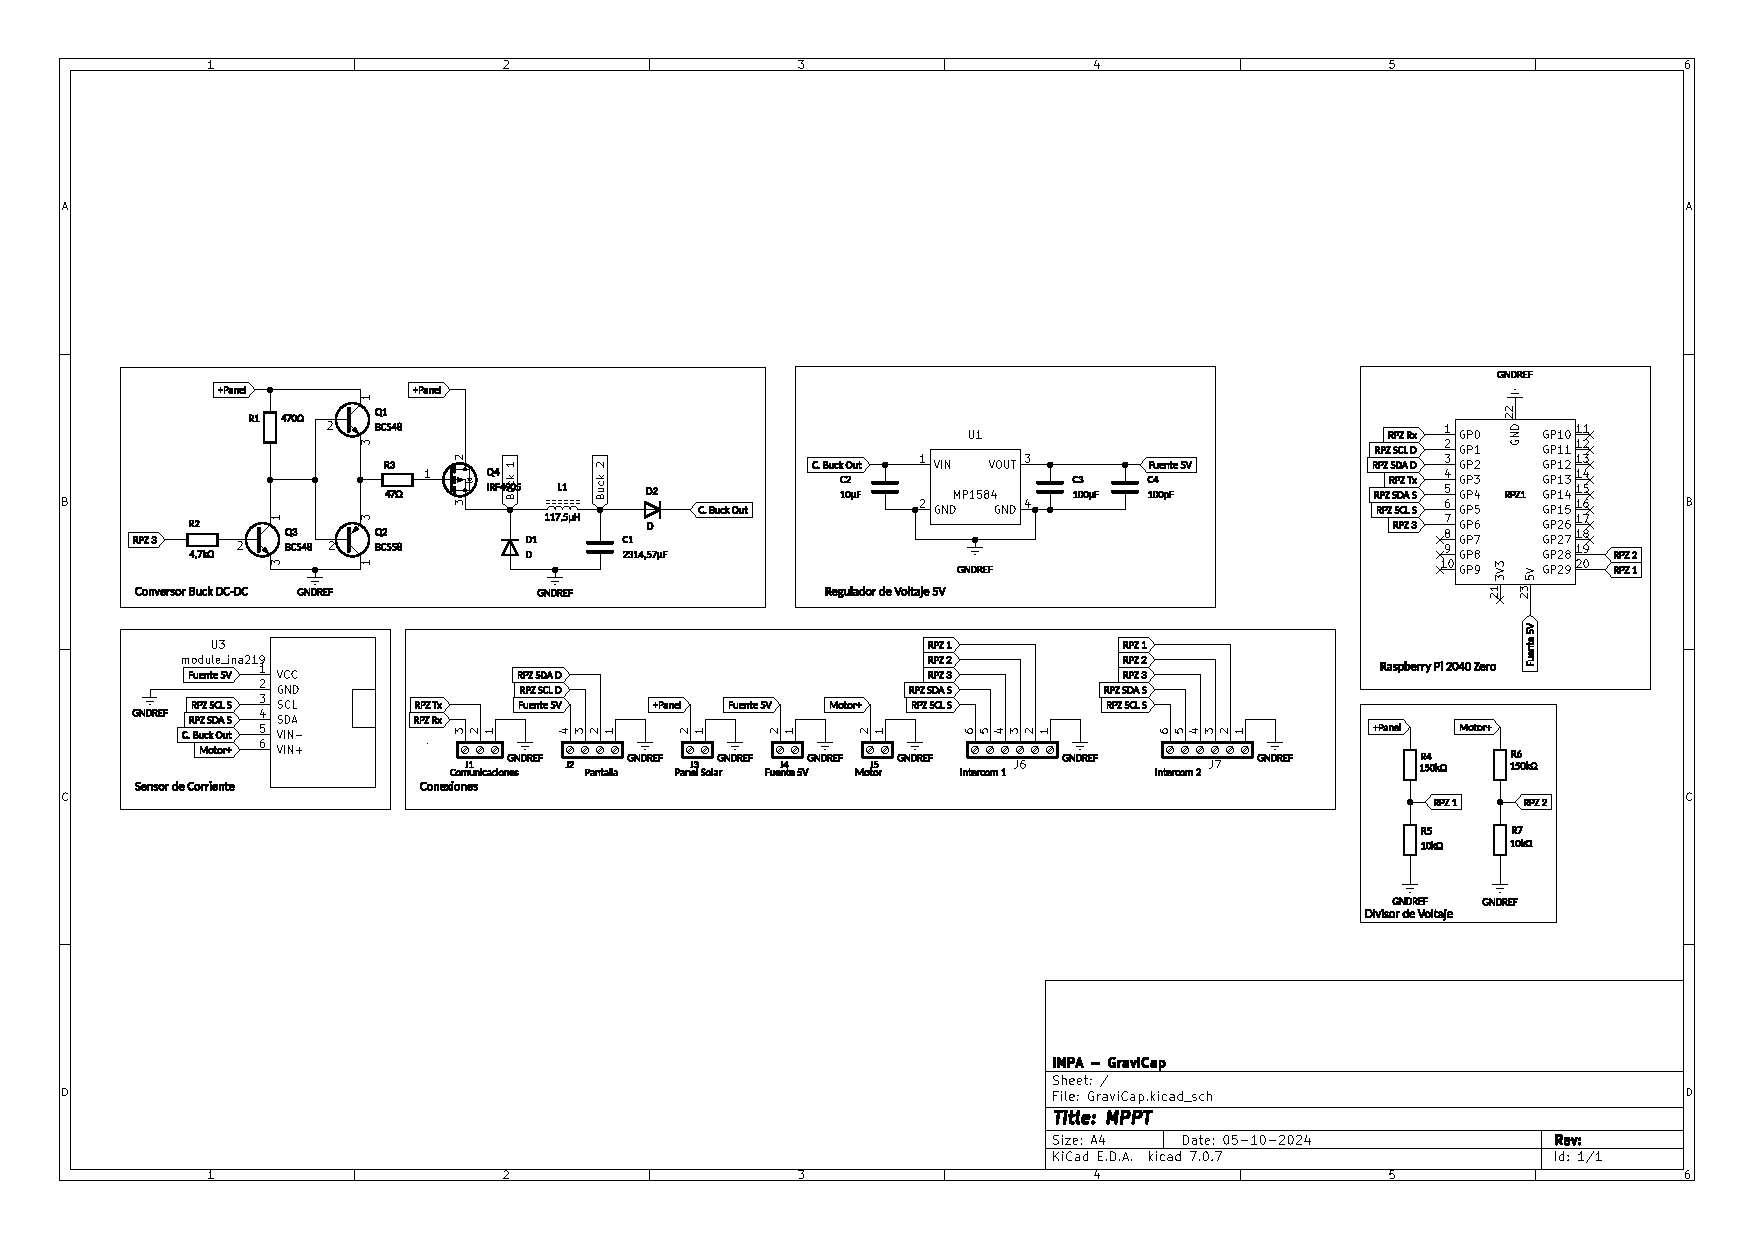
\includegraphics[angle=270, width=\textwidth,height=\textheight,keepaspectratio]{Anexo_A/Esquemático - MPPT.pdf}
            \label{fig:A_1}
        \end{sidewaysfigure}
        
        \newpage

        \begin{sidewaysfigure}
            \centering
            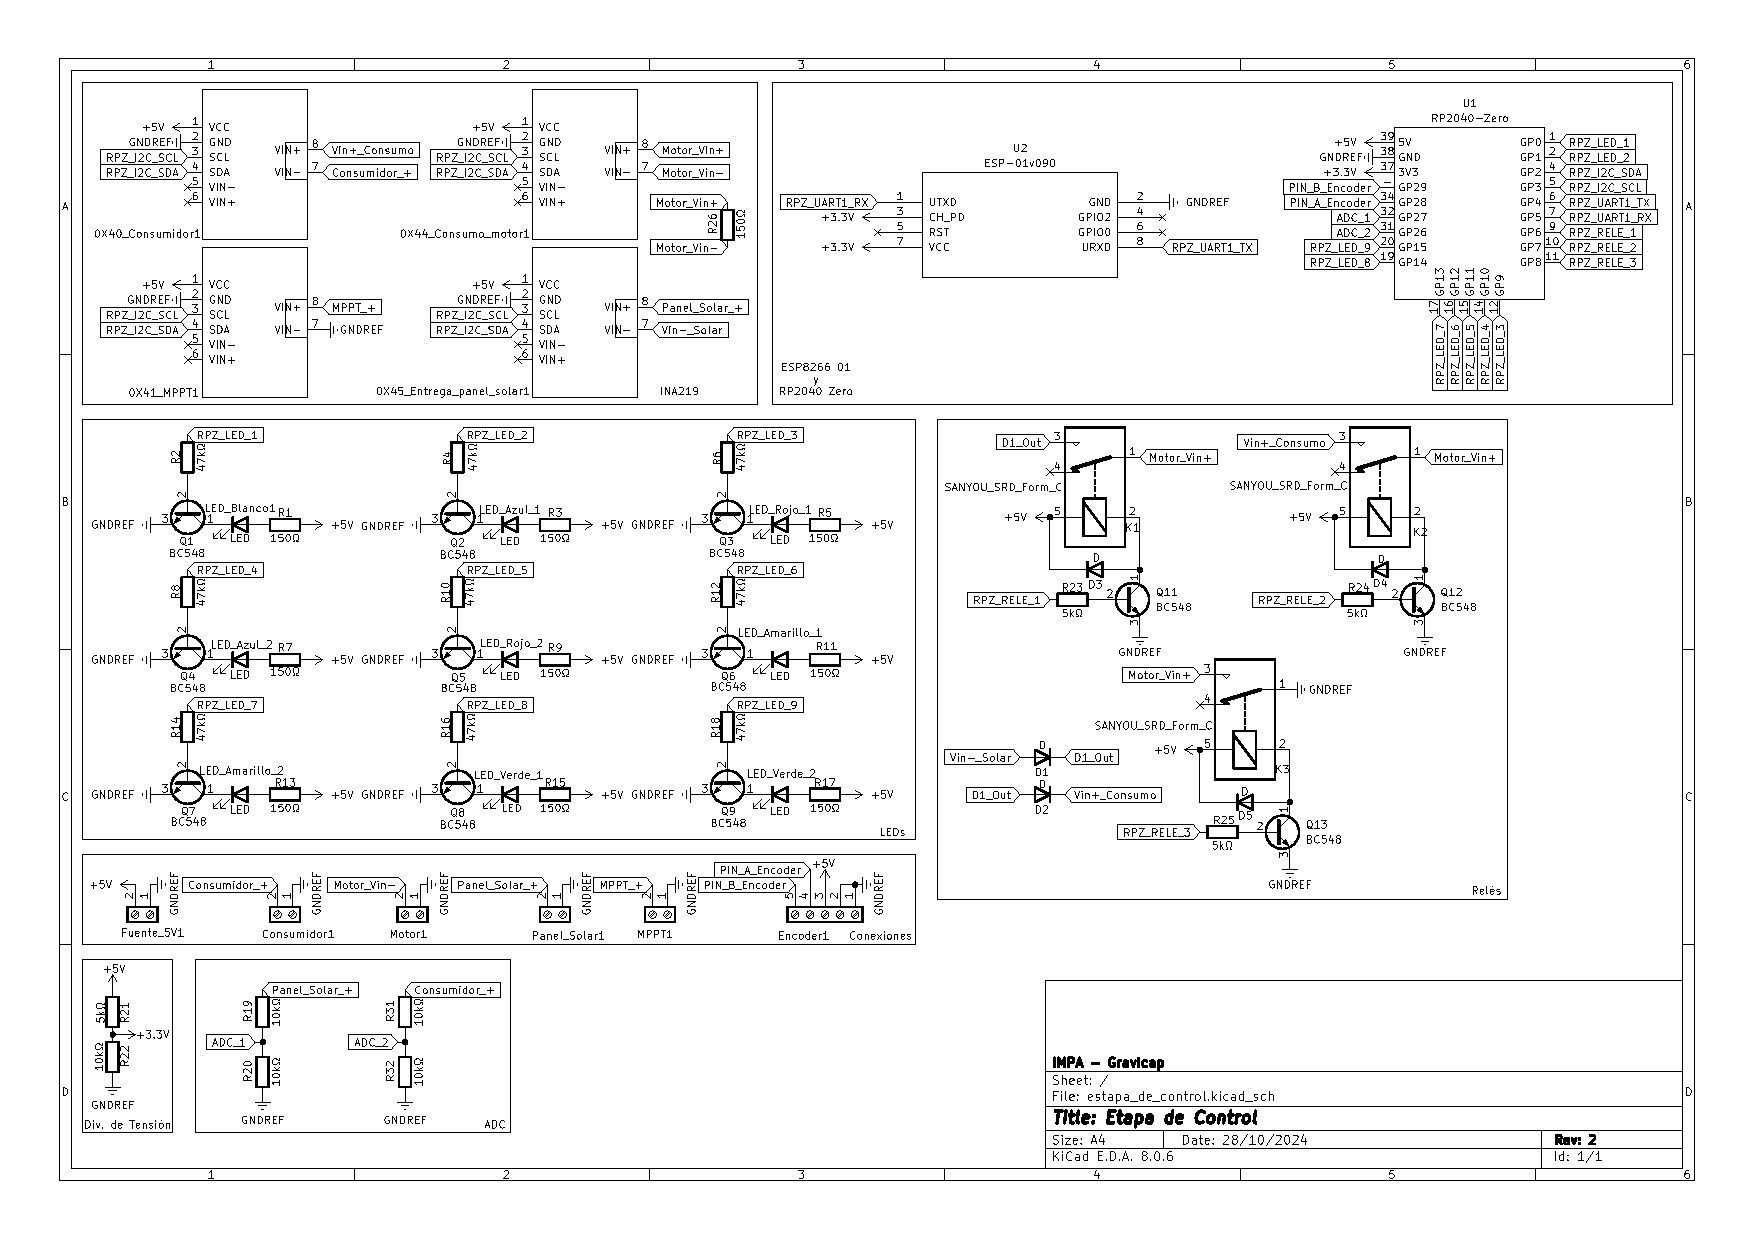
\includegraphics[angle=270, width=\textwidth,height=\textheight,keepaspectratio]{Anexo_A/Esquemático - Etapa_de_Control.pdf}
            \label{fig:A_2}
        \end{sidewaysfigure}
        
    \end{landscape}

\chapter{Apéndice B: Códigos}
\renewcommand{\thepage}{B-\arabic{page}}
\setcounter{page}{1}
    \section{MPPT}
    
        \lstinputlisting[language=C, caption=\texttt{main.c} del MPPT]{main.c}
        \label{Listing B.1}
        
    \section{Etapa de Control}
        \lstinputlisting[language=C, caption=\texttt{main.c} de la Etapa de Control]{maino.c}
        \label{Listing B.2}
        
        \lstinputlisting[language=C, caption=\texttt{gravi.c} de la Etapa de Control]{gravi.c}
        \label{Listing B.3}

        \lstinputlisting[language=C, caption=\texttt{gravi.h} de la Etapa de Control]{gravi.h}
        \label{Listing B.4}

\include{Anexo_c}

\end{appendix}

\end{document}